




%----------------------------------------------------------------------------------------

\newpage

%%%%%%%%%%%%%%%%%%%%%%%
\section{Aggregation-diffusion morphogenesis}{Morphogenèse par agrégation-diffusion}

\label{app:sec:density}




%%%%%%%%%%%%%%%%%%%%%%%
\subsection{Extended Figures for Model Exploration}{Figures supplémentaires pour l'exploration du modèle}


\subsubsection{Convergence}{Convergence}


\bpar{
Histograms for the 81 parameters points for which we did 100 repetitions are given in Fig.~\ref{fig:app:density:histograms}, for Moran index and slope indicators. Other indicators showed similar convergence patterns. The visual exploration of histograms confirms the numerical analysis done in main text for statistical convergence.
}{
Les histogrammes pour les 81 points de paramètres pour lesquelles 100 répétitions ont été menées sont donnés en Fig.~\ref{fig:app:density:histograms}, pour l'index de Moran et la hiérarchie. Les autres indicateurs témoignent de propriétés de convergence similaires. L'exploration visuelle des histogrammes confirme l'analyse numérique menée dans le texte principal pour la convergence statistique.
}


% histograms


% and bimodal statistical distribution for cumulated points in the parameter space confirm the existence of superposed regimes : gaussian distribution gives stationary configurations, whereas inverse log-normal distribution are close to real data shape and correspond to non-stationary regime.
% -> not sure it is interesting to look at cumulated histograms.

% Figures :

%%%%%%%%%%%%%%%%%%%%
\begin{figure}
%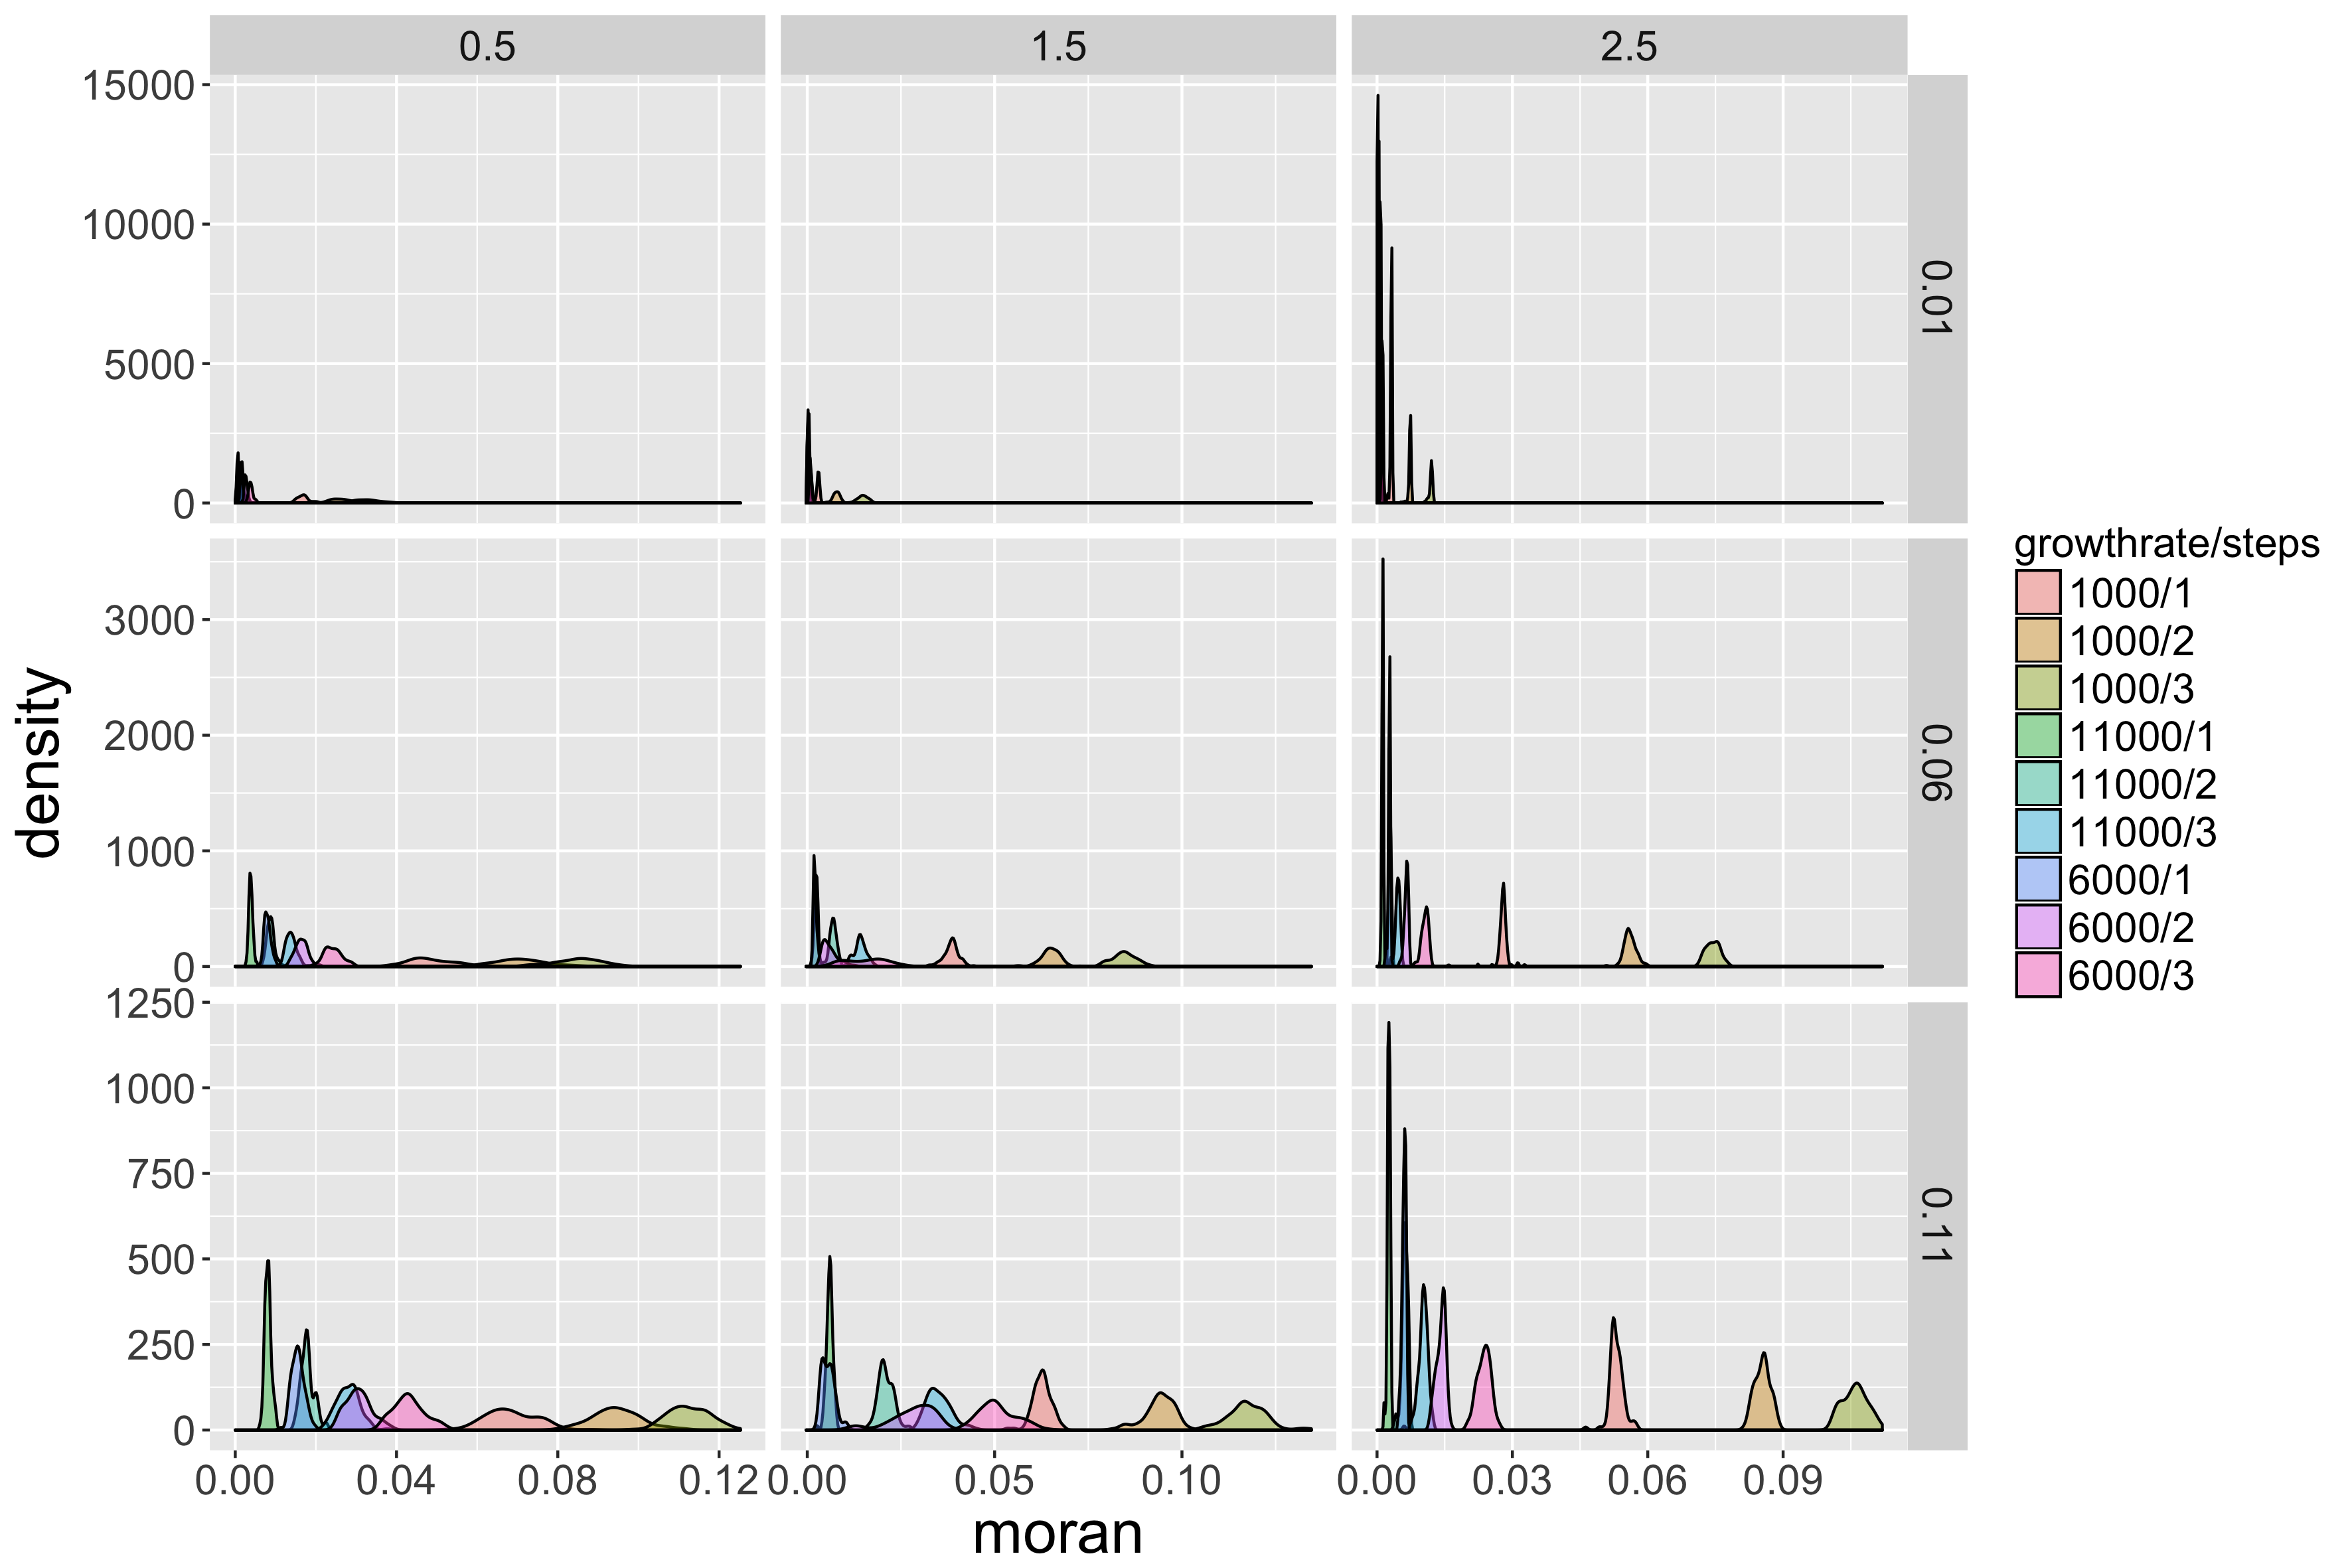
\includegraphics[width=0.8\textwidth]{Figures/Density/hist_moran.png}\\
%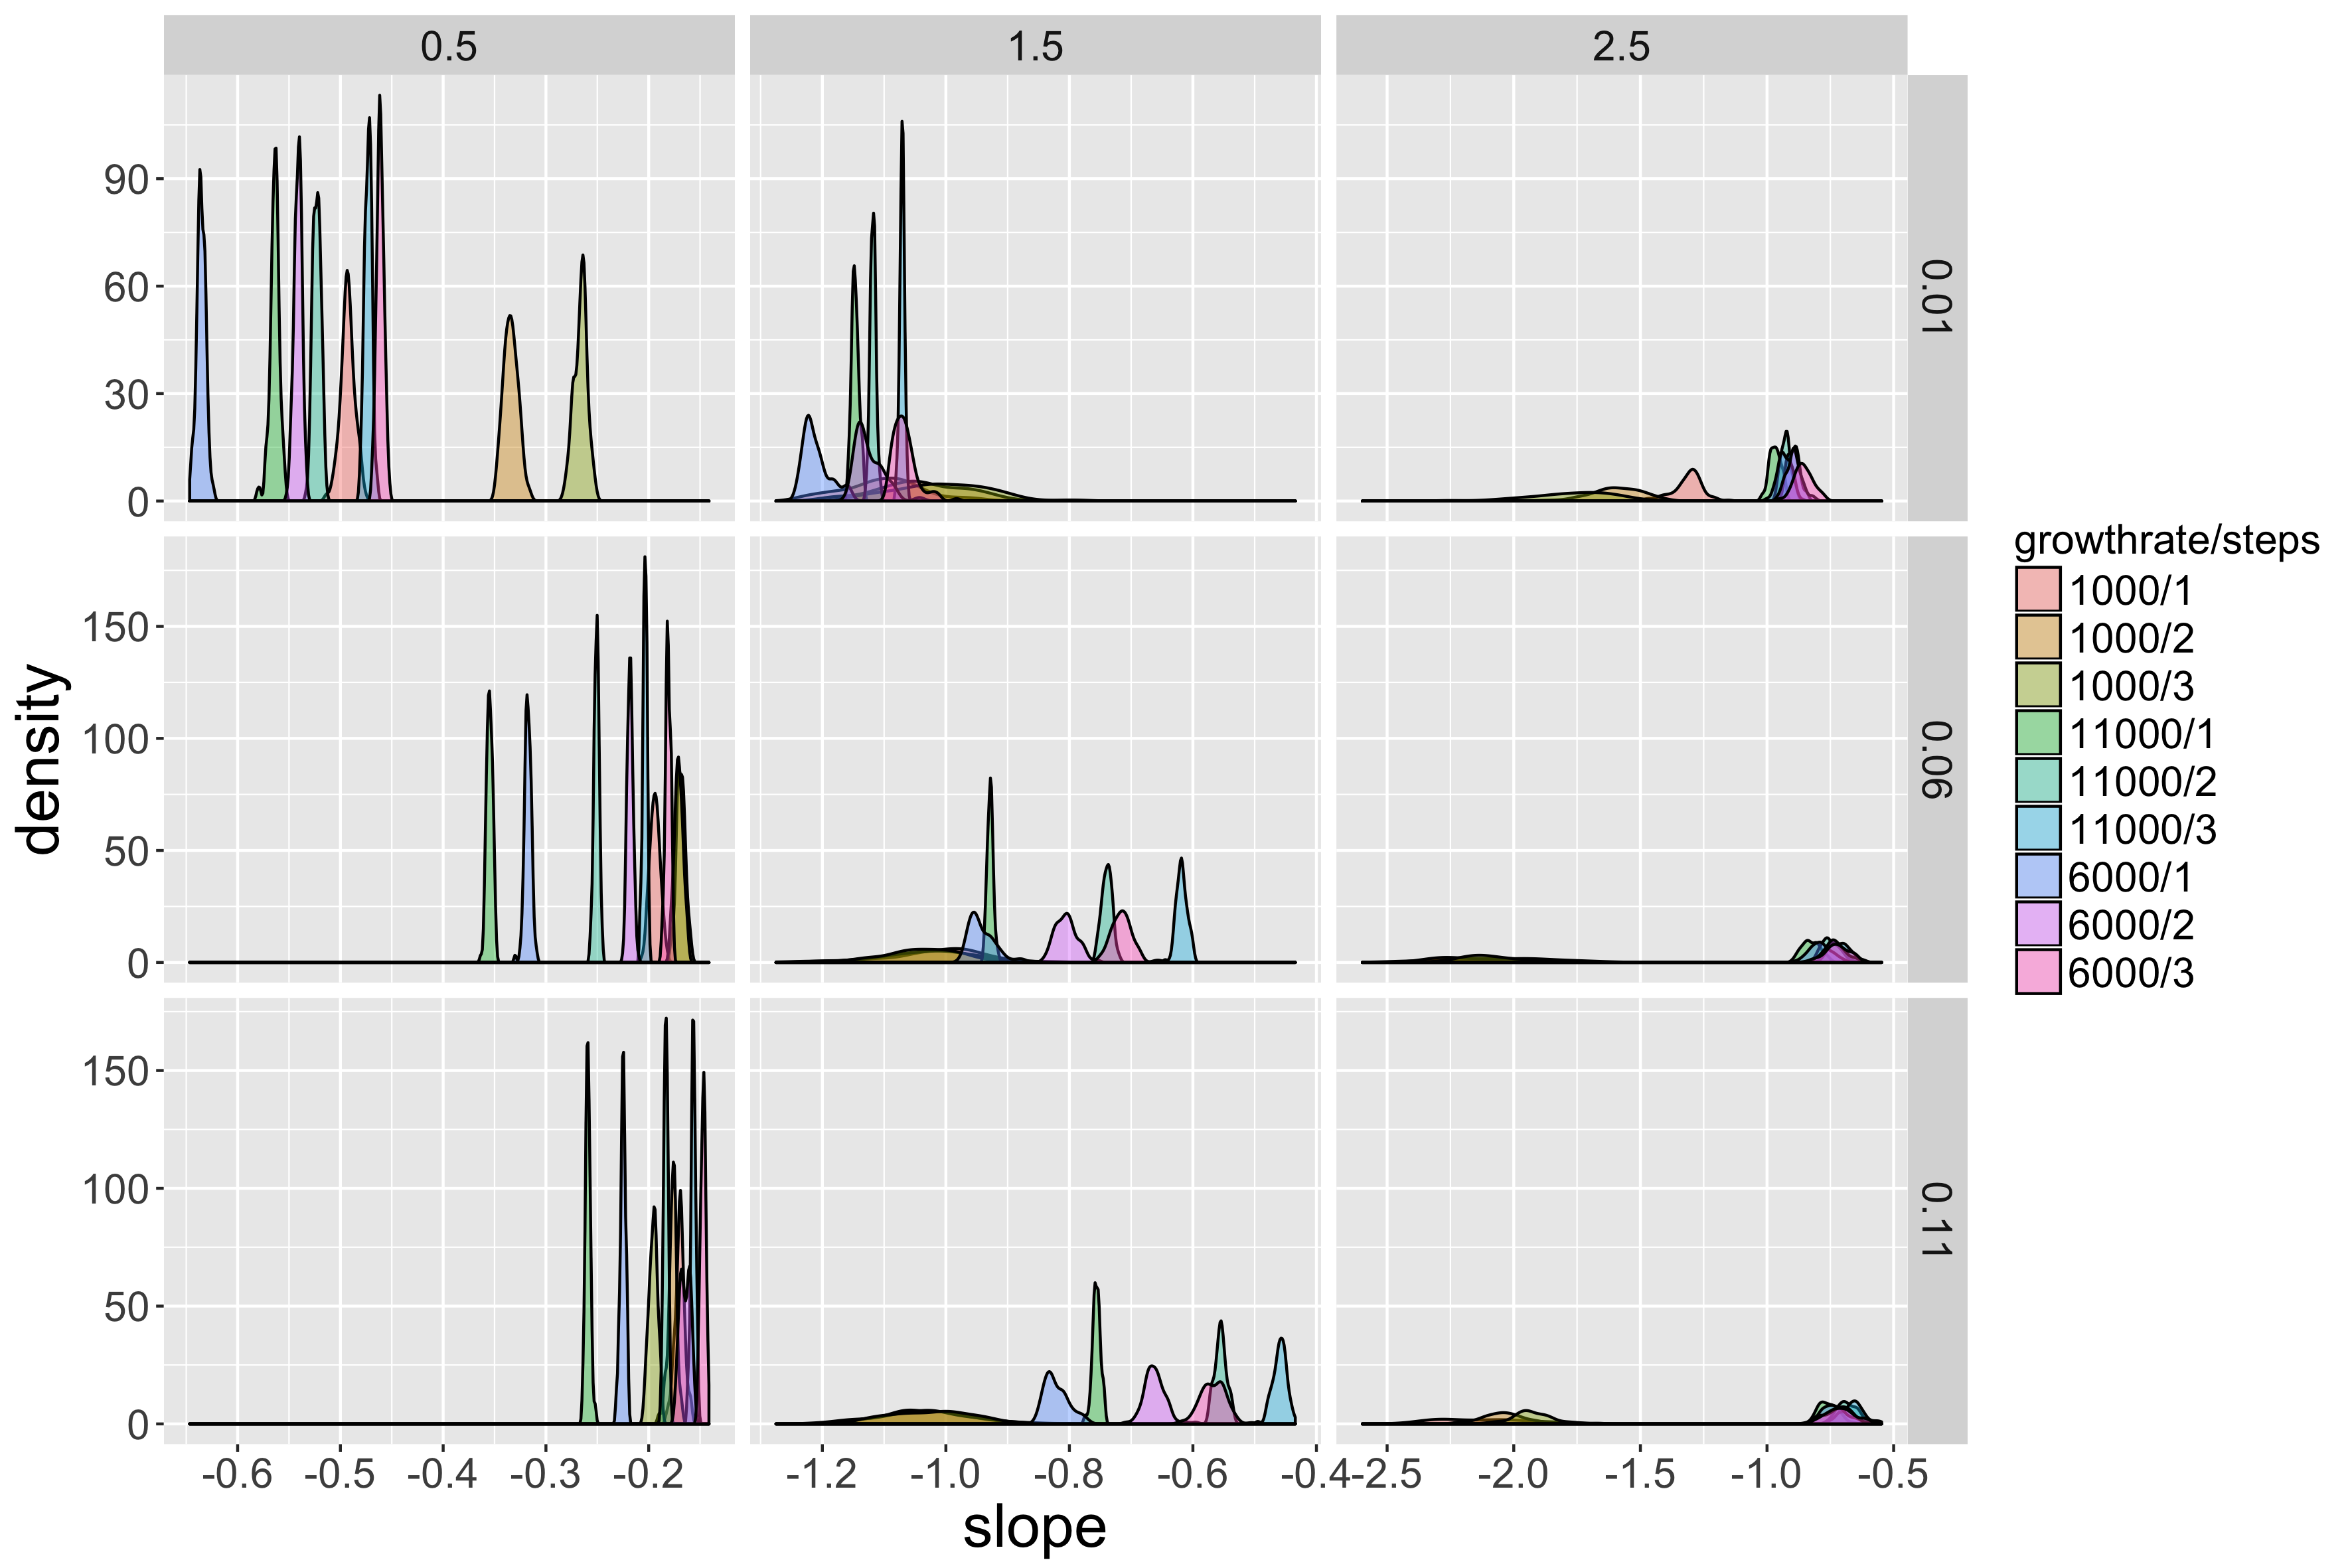
\includegraphics[width=0.8\textwidth]{Figures/Density/hist_slope.png}
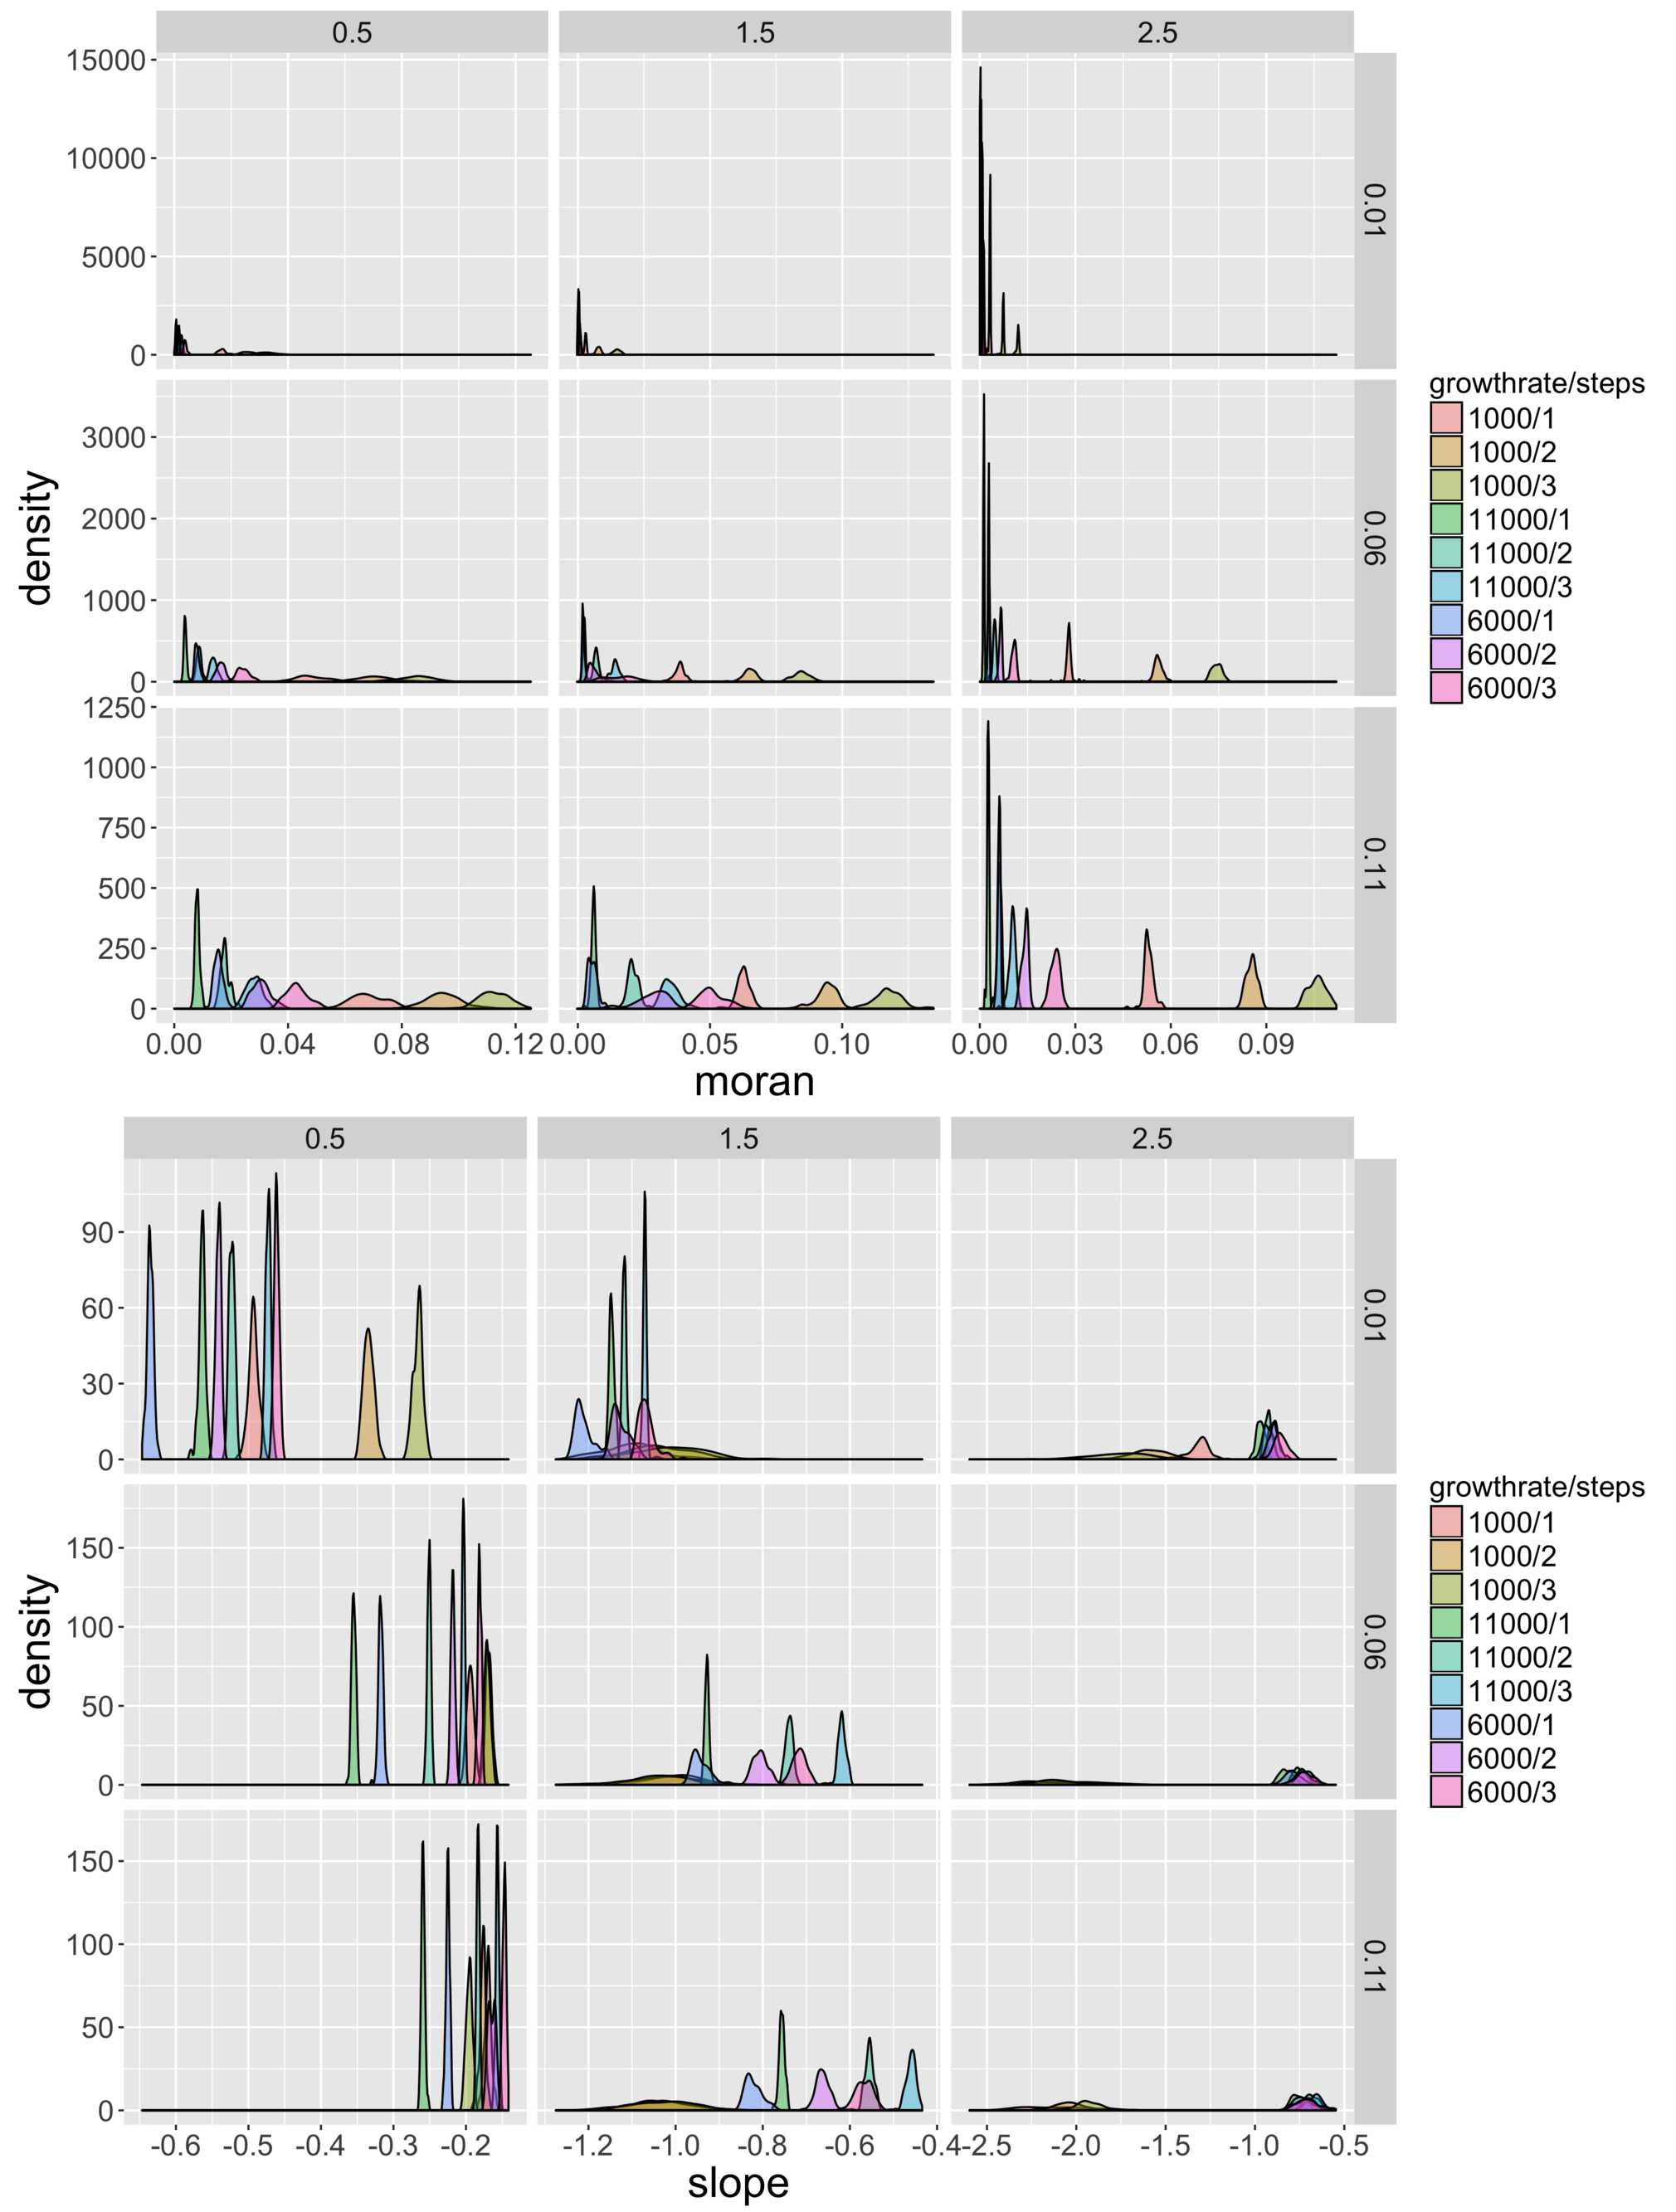
\includegraphics[width=\linewidth]{Figures/Final/A-density-histograms.jpg}
\appcaption{Histograms for Moran index (top) and slope (bottom), for varying $\alpha$ (columns), $\beta$ (rows), $N_G$ and $n_d$ (colors).}{\textit{(Haut)} Distributions de l'Index de Moran, pour des valeurs variables de $\alpha$ (colonnes), $\beta$ (lignes), $N_G$ et $n_d$ (couleurs)\label{fig:app:density:histograms}}
\end{figure}
%%%%%%%%%%%%%%%%%%%%






\subsubsection{Indicators Behavior}{Indicateurs}

% full plots behavior


\bpar{
We show in Fig.~\ref{fig:app:density:moran} to Fig.~\ref{fig:app:density:entropy} the full behavior of all indicators, with all parameters varying, obtained through the extensive exploration, from which the plots in main text have been extracted. Because of the complex nature of emergent urban form, one can not predict output values without referring to this ``exhaustive'' parameter sweep.
}{
Nous donnons en Fig.~\ref{fig:app:density:moran} à Fig.~\ref{fig:app:density:entropy} le comportement exhaustif des indicateurs, pour l'ensemble des paramètres variant. Ceux-ci ont été obtenus par l'exploration intensive, et les graphiques en texte principal en sont des cas particuliers. A cause de la nature complexe de la forme urbaine émergente, il n'est pas possible de prédire les valeurs de sorties sans référer à cette exploration ``exhaustive'' de l'espace des paramètres.
}


%%%%%%%%%%%%%%%%%%%%
\begin{figure}
%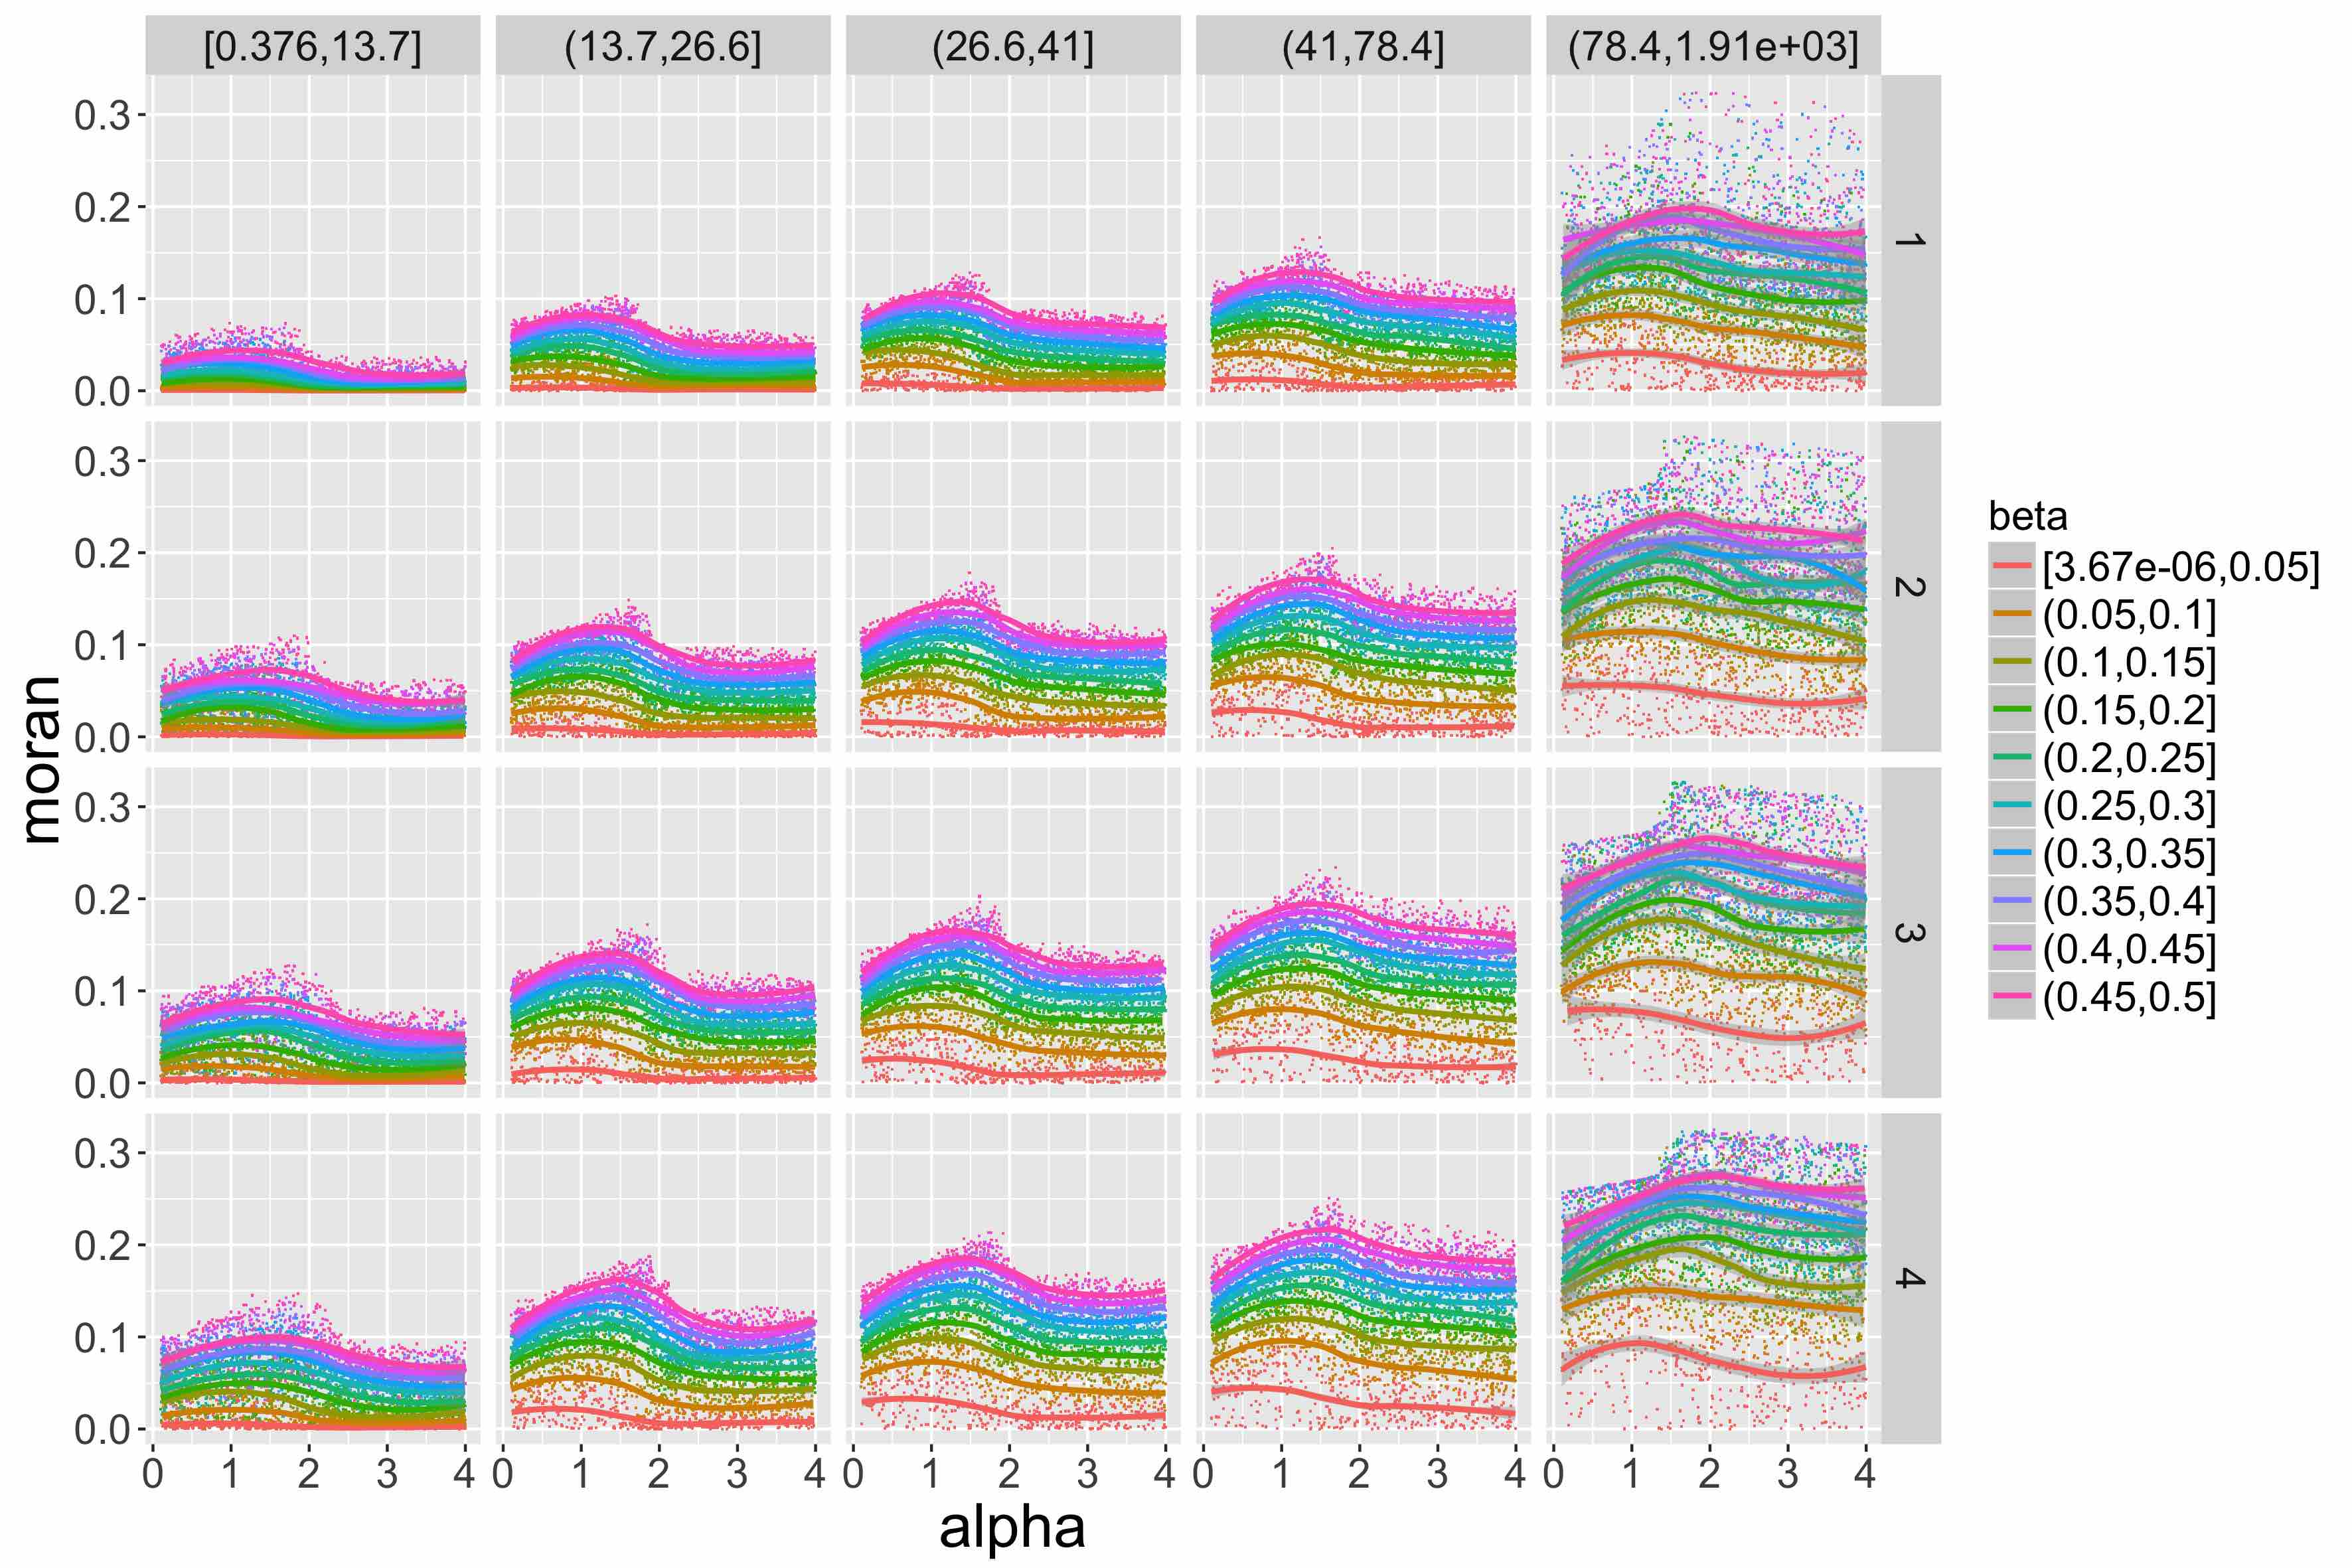
\includegraphics[width=0.8\textwidth]{Figures/Density/moran_alpha}
%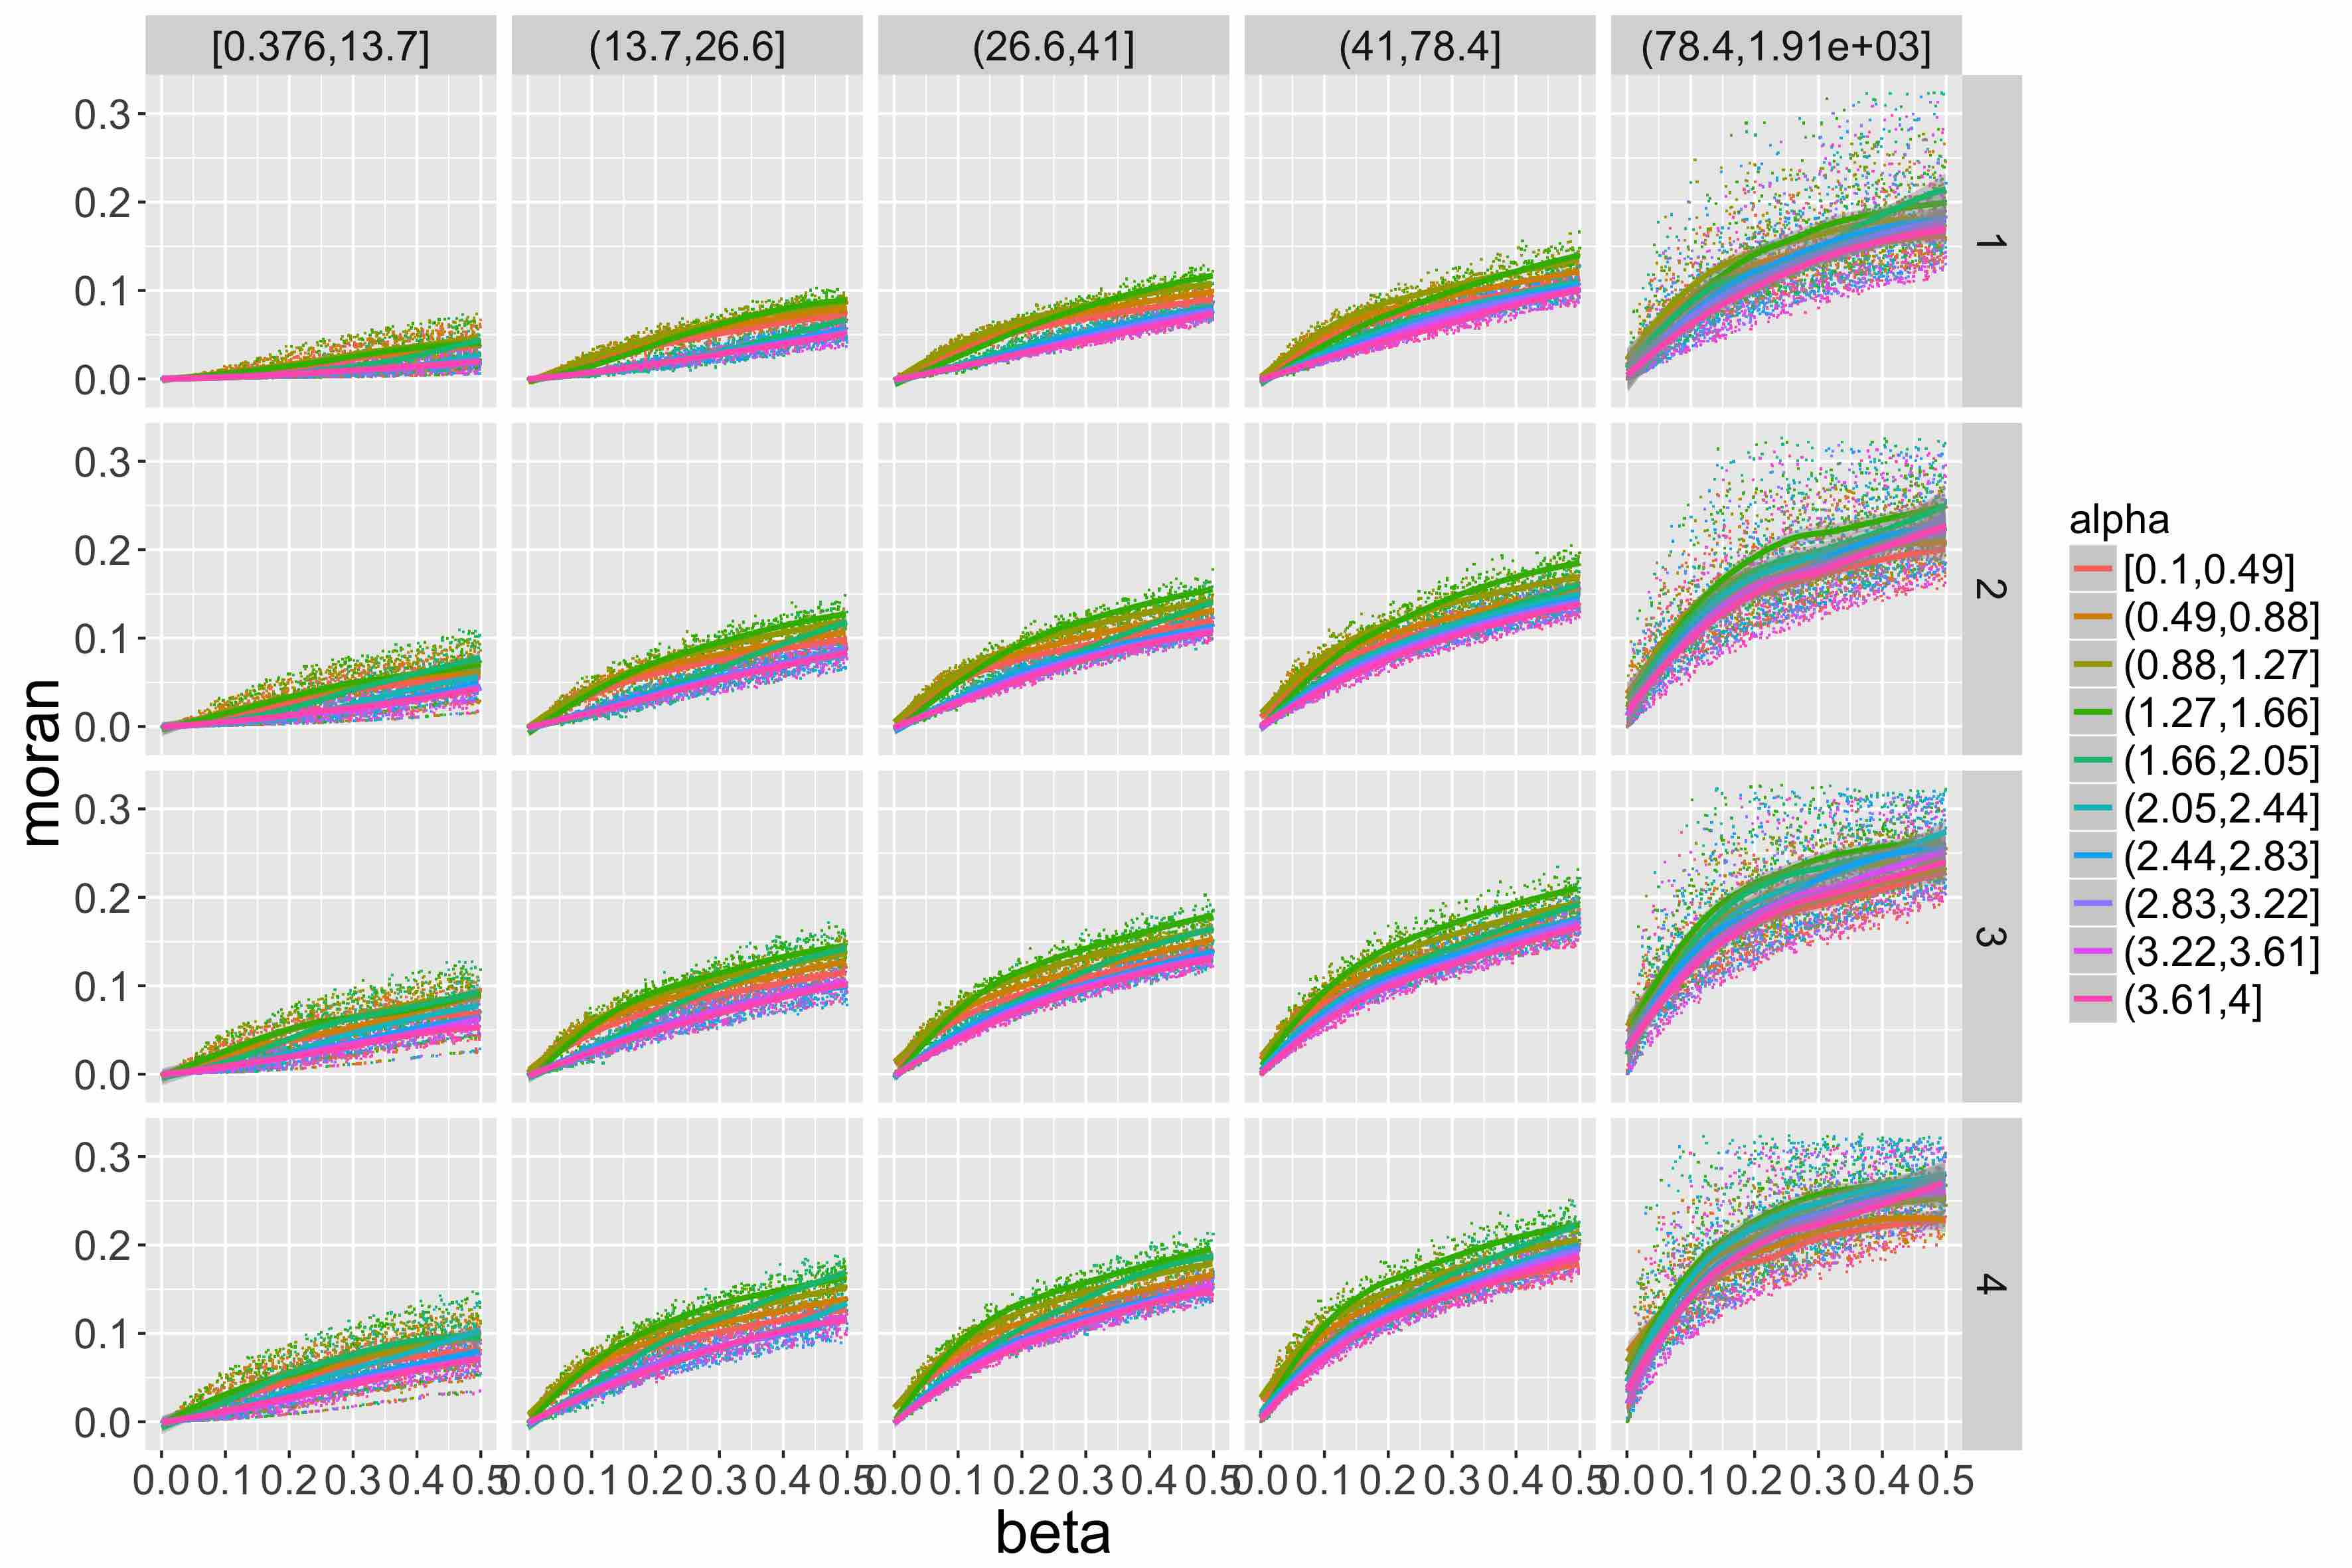
\includegraphics[width=0.8\textwidth]{Figures/Density/moran_beta}
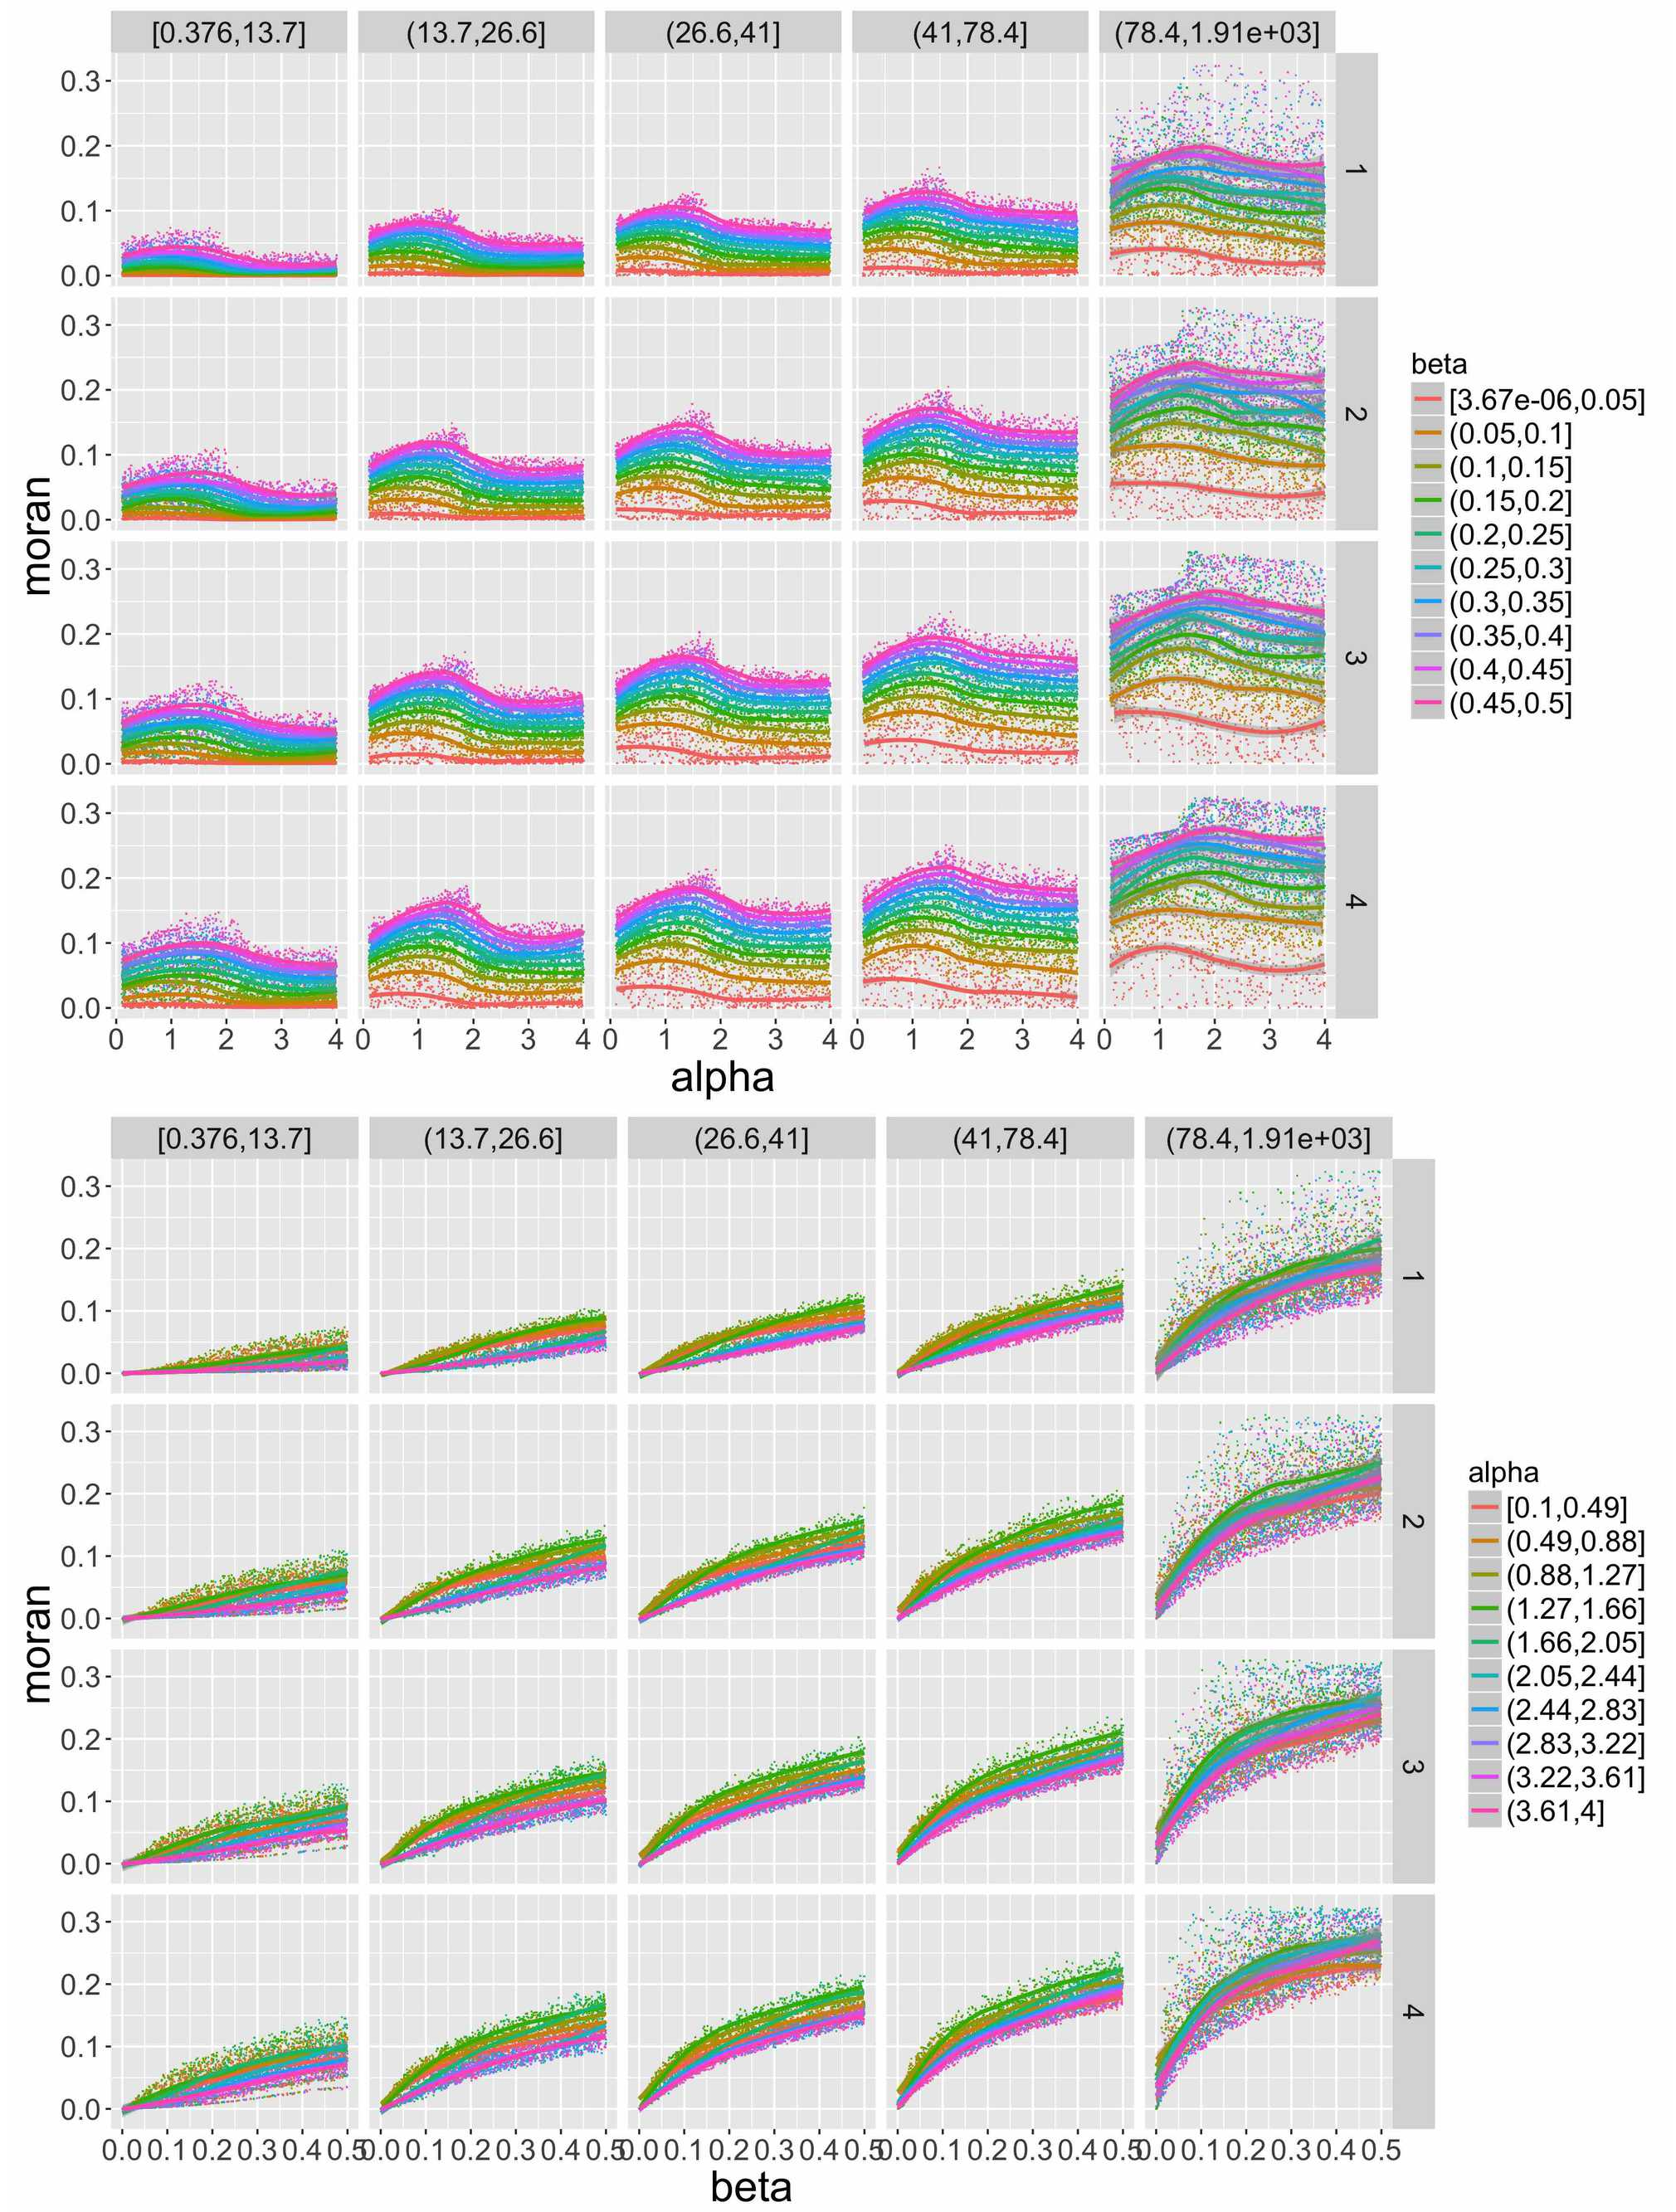
\includegraphics[width=\linewidth]{Figures/Final/A-density-moran.jpg}
\appcaption{Moran index as a function of $\alpha$ (Top) and $\beta$ (Bottom) for varying $\beta$ (resp. $\alpha$) given by color, and varying $n_d$ (rows) and $N_G$ (columns).}{Indice de Moran en fonction de $\alpha$ (Haut) et $\beta$ (Bas) pour $\beta$ variable (resp. $\alpha$) donné par la couleur, et $n_d$ (lignes) et $N_G$ (colonnes) variables.\label{fig:app:density:moran}}
\end{figure}
%%%%%%%%%%%%%%%%%%%%


%%%%%%%%%%%%%%%%%%%%
\begin{figure}
%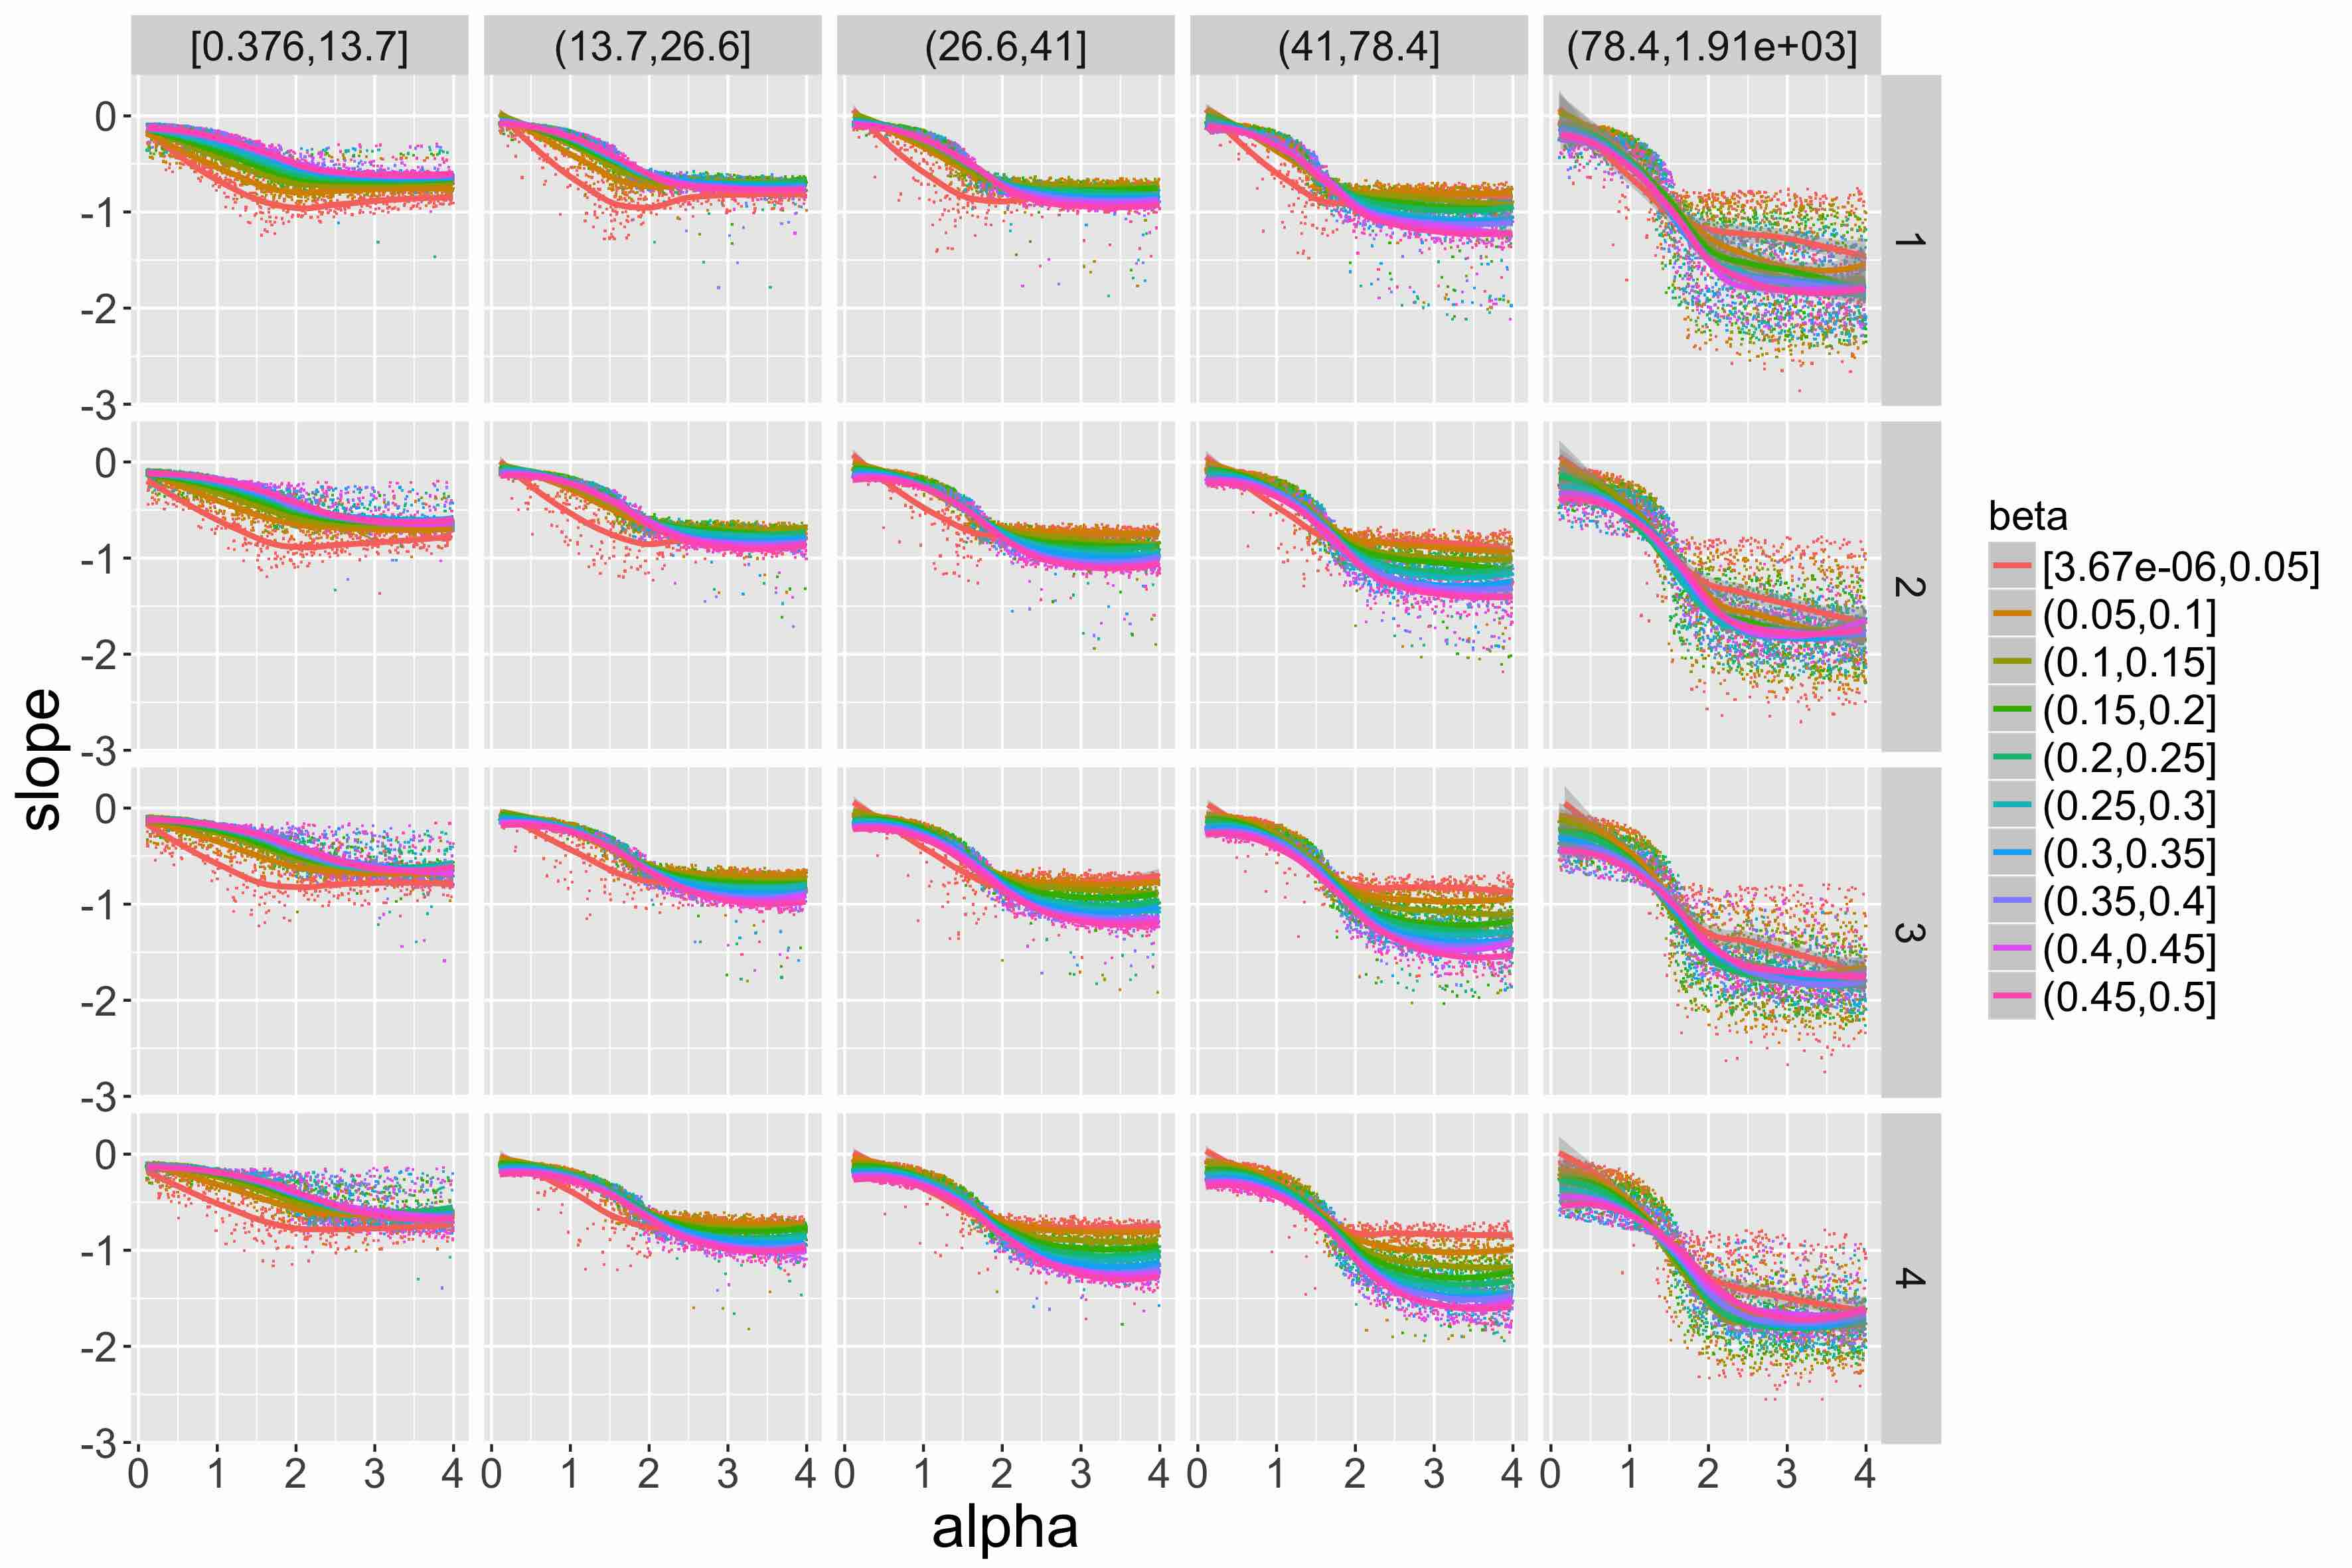
\includegraphics[width=0.8\textwidth]{Figures/Density/slope_alpha}
%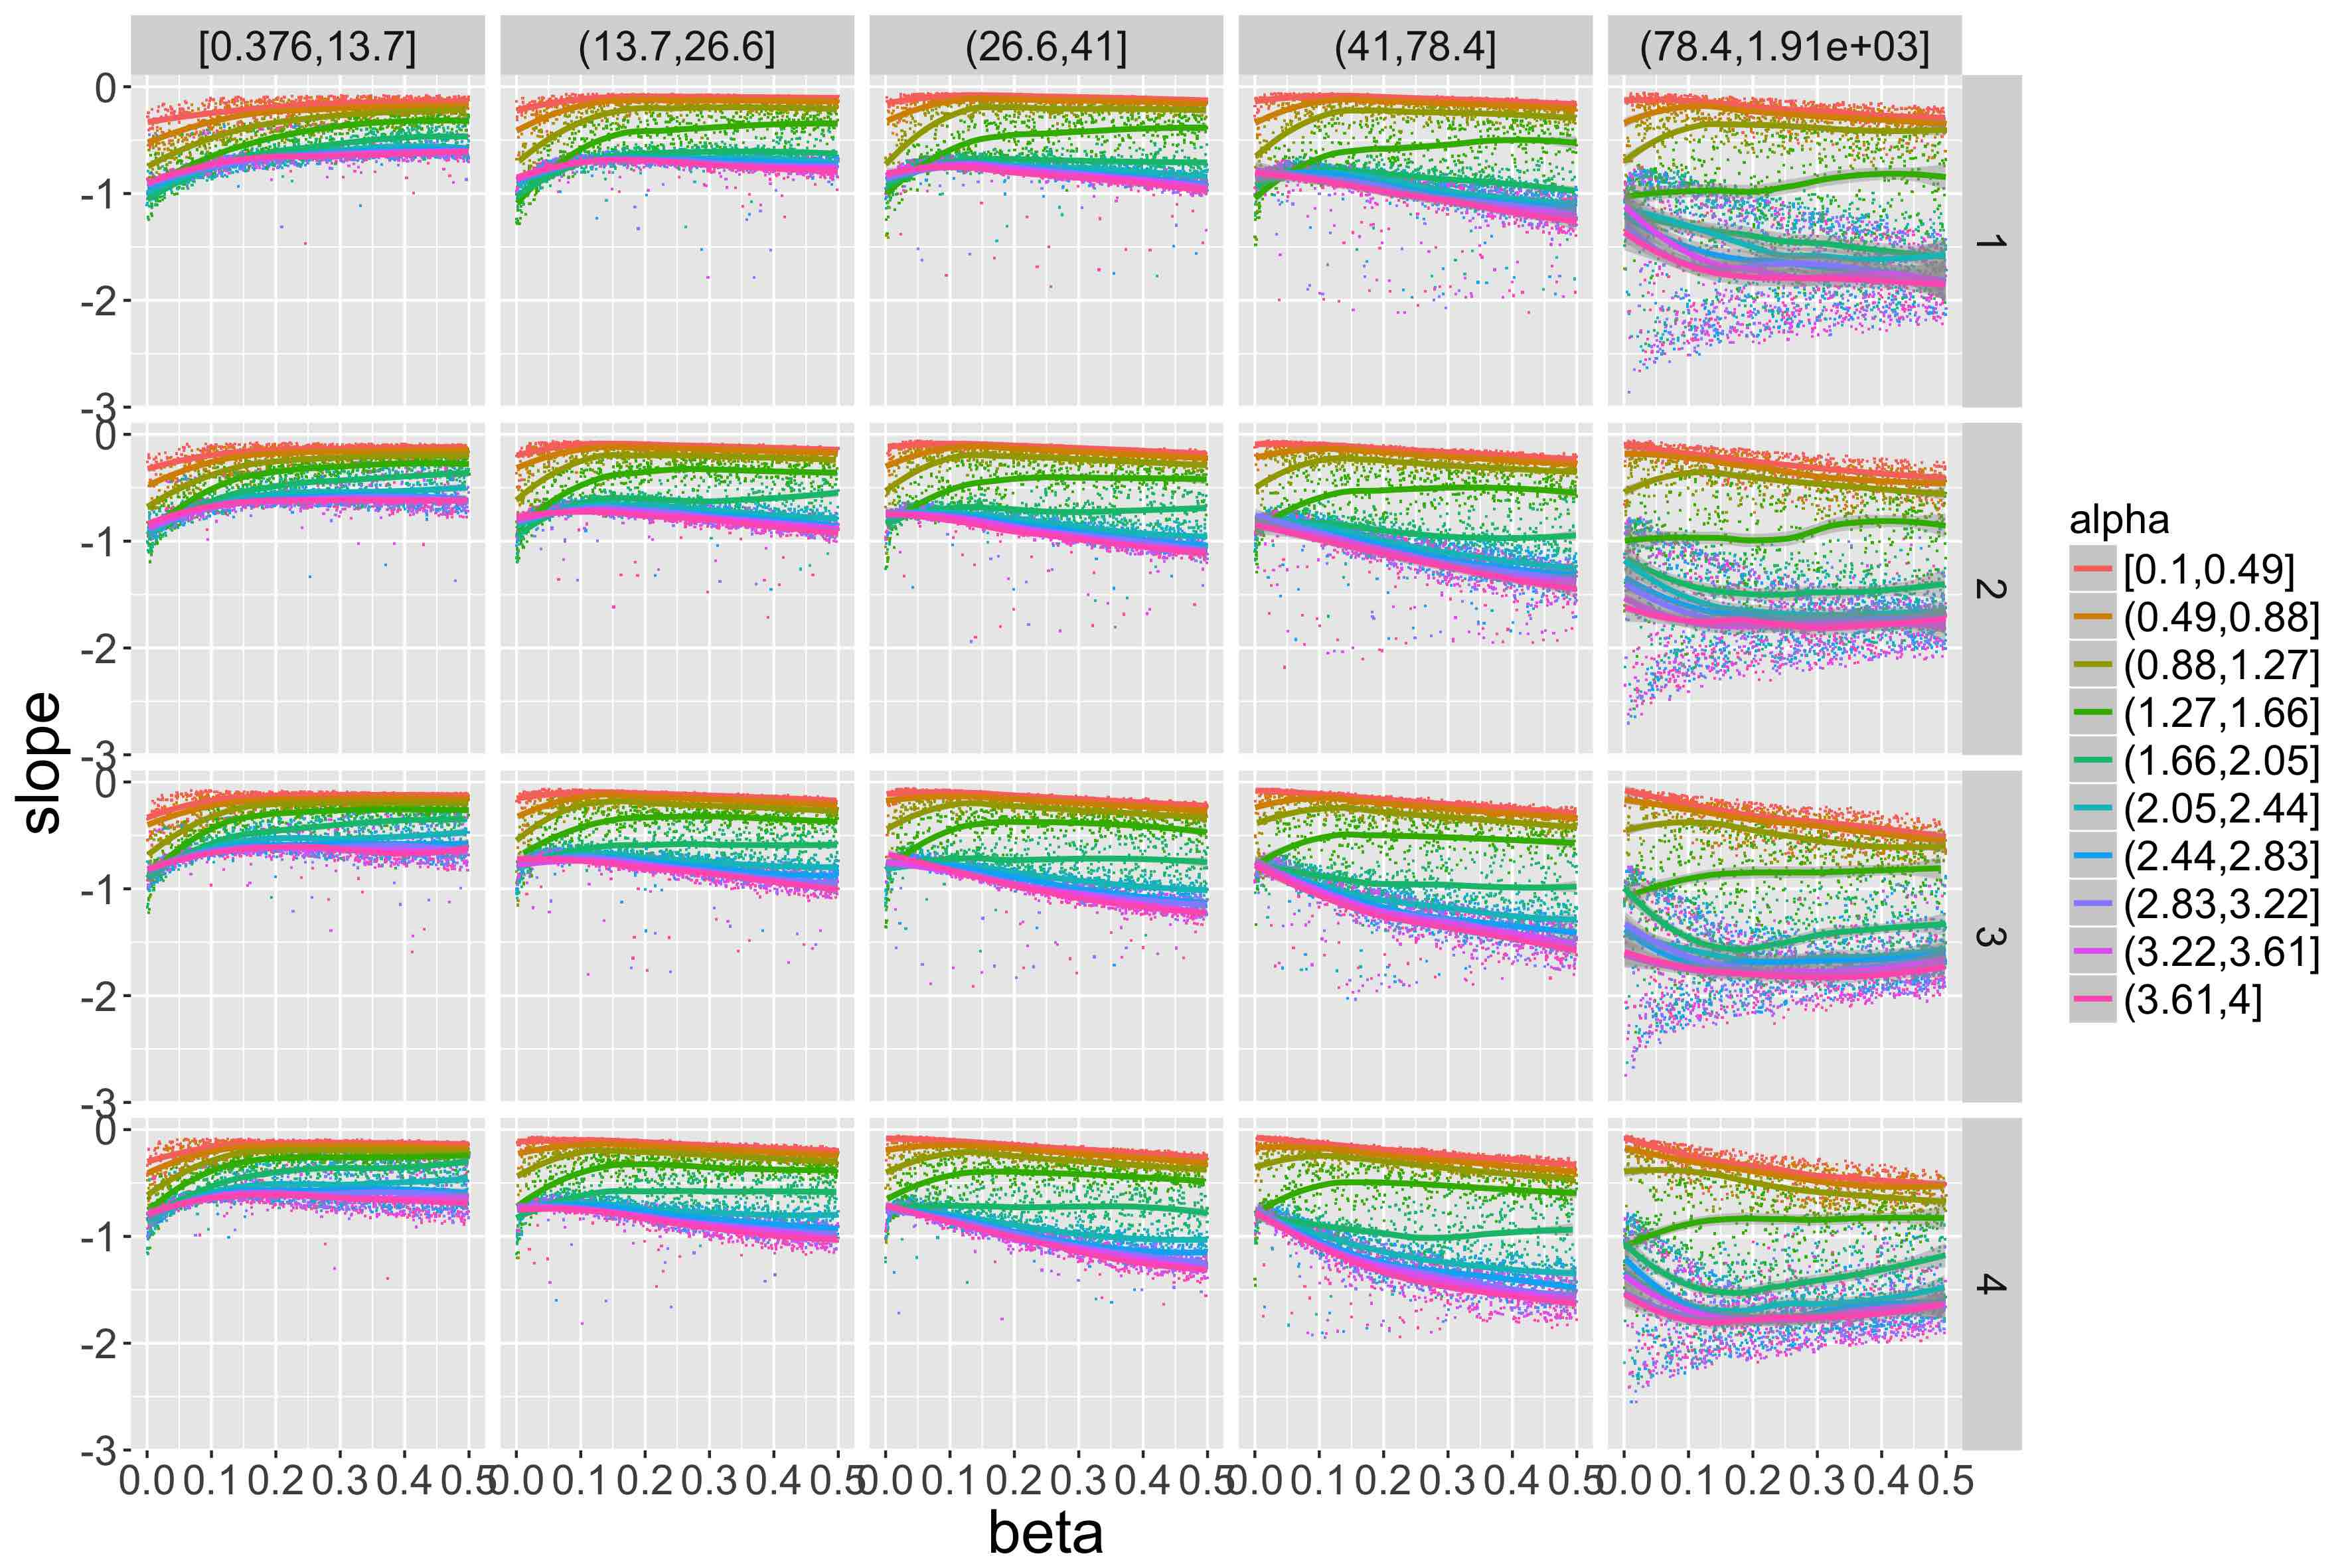
\includegraphics[width=0.8\textwidth]{Figures/Density/slope_beta}
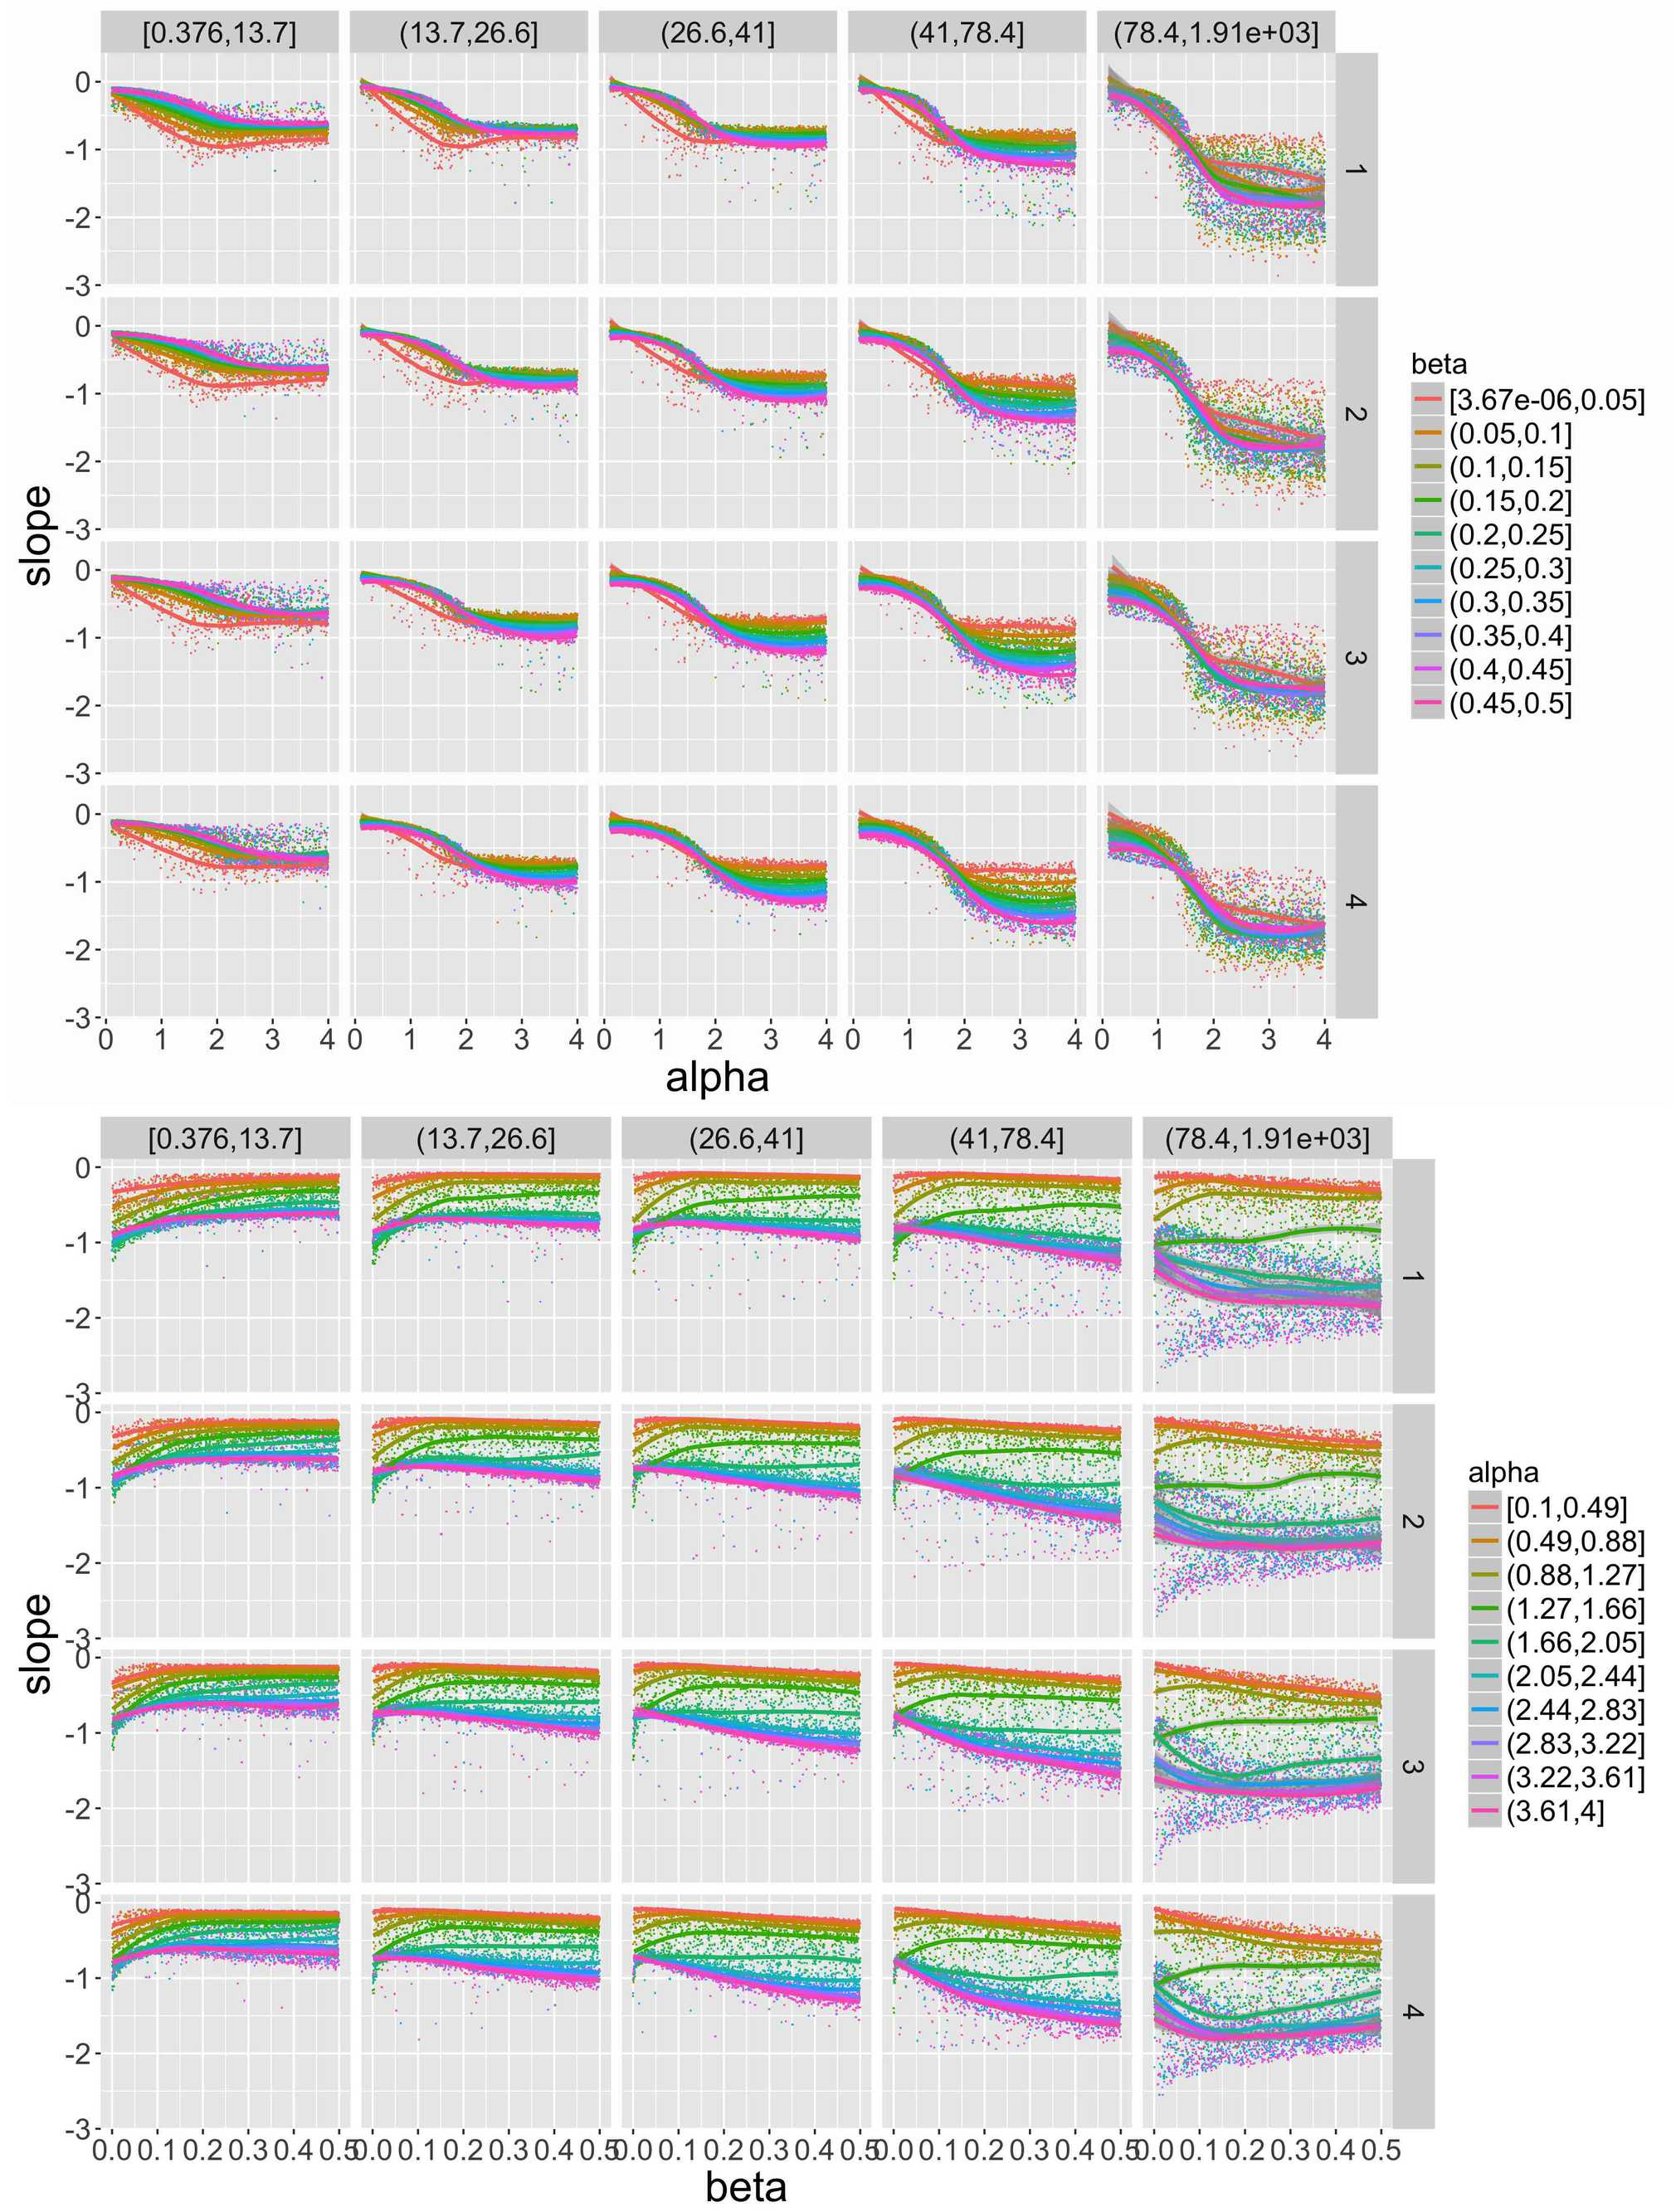
\includegraphics[width=\linewidth]{Figures/Final/A-density-slope.jpg}
\appcaption{Slope as a function of $\alpha$ (Top) and $\beta$ (Bottom) for varying $\beta$ (resp. $\alpha$) given by color, and varying $n_d$ (rows) and $N_G$ (columns).}{Hiérarchie en fonction de $\alpha$ (Haut) et $\beta$ (Bas) pour $\beta$ variable (resp. $\alpha$) donné par la couleur, et $n_d$ (lignes) et $N_G$ (colonnes) variables.\label{fig:app:density:slope}}
\end{figure}
%%%%%%%%%%%%%%%%%%%%


%%%%%%%%%%%%%%%%%%%%
\begin{figure}
%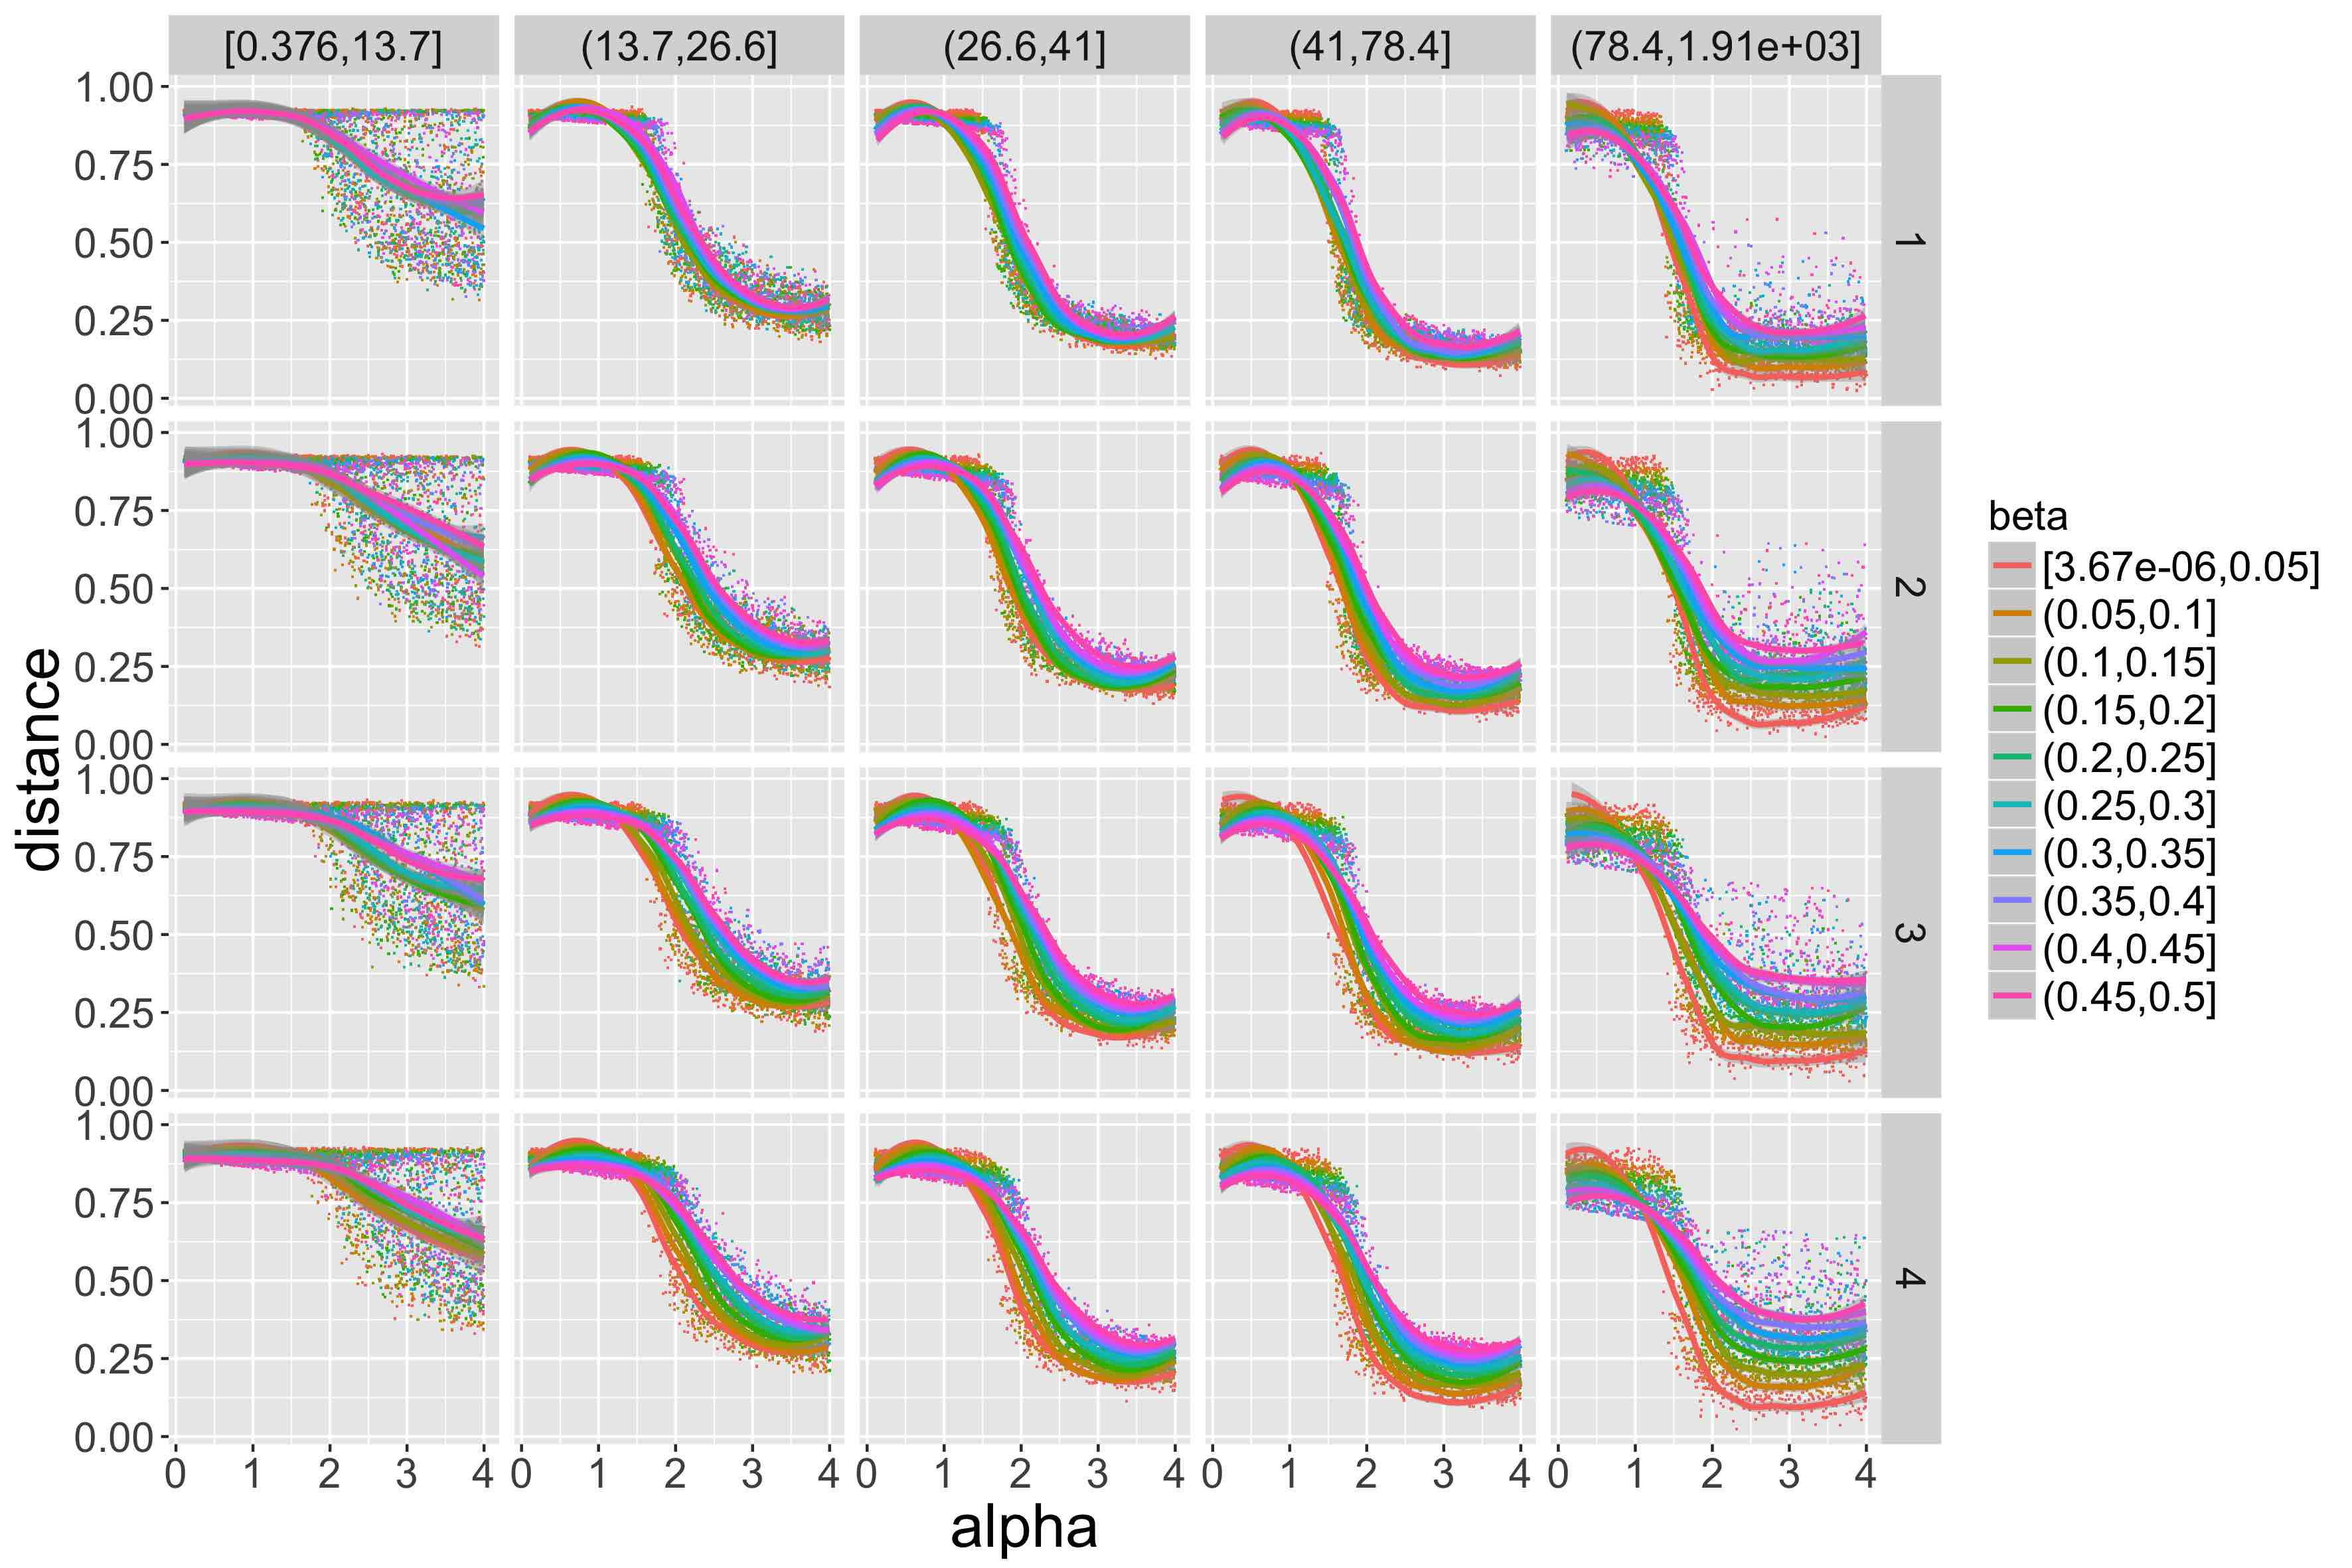
\includegraphics[width=0.8\textwidth]{Figures/Density/distance_alpha}
%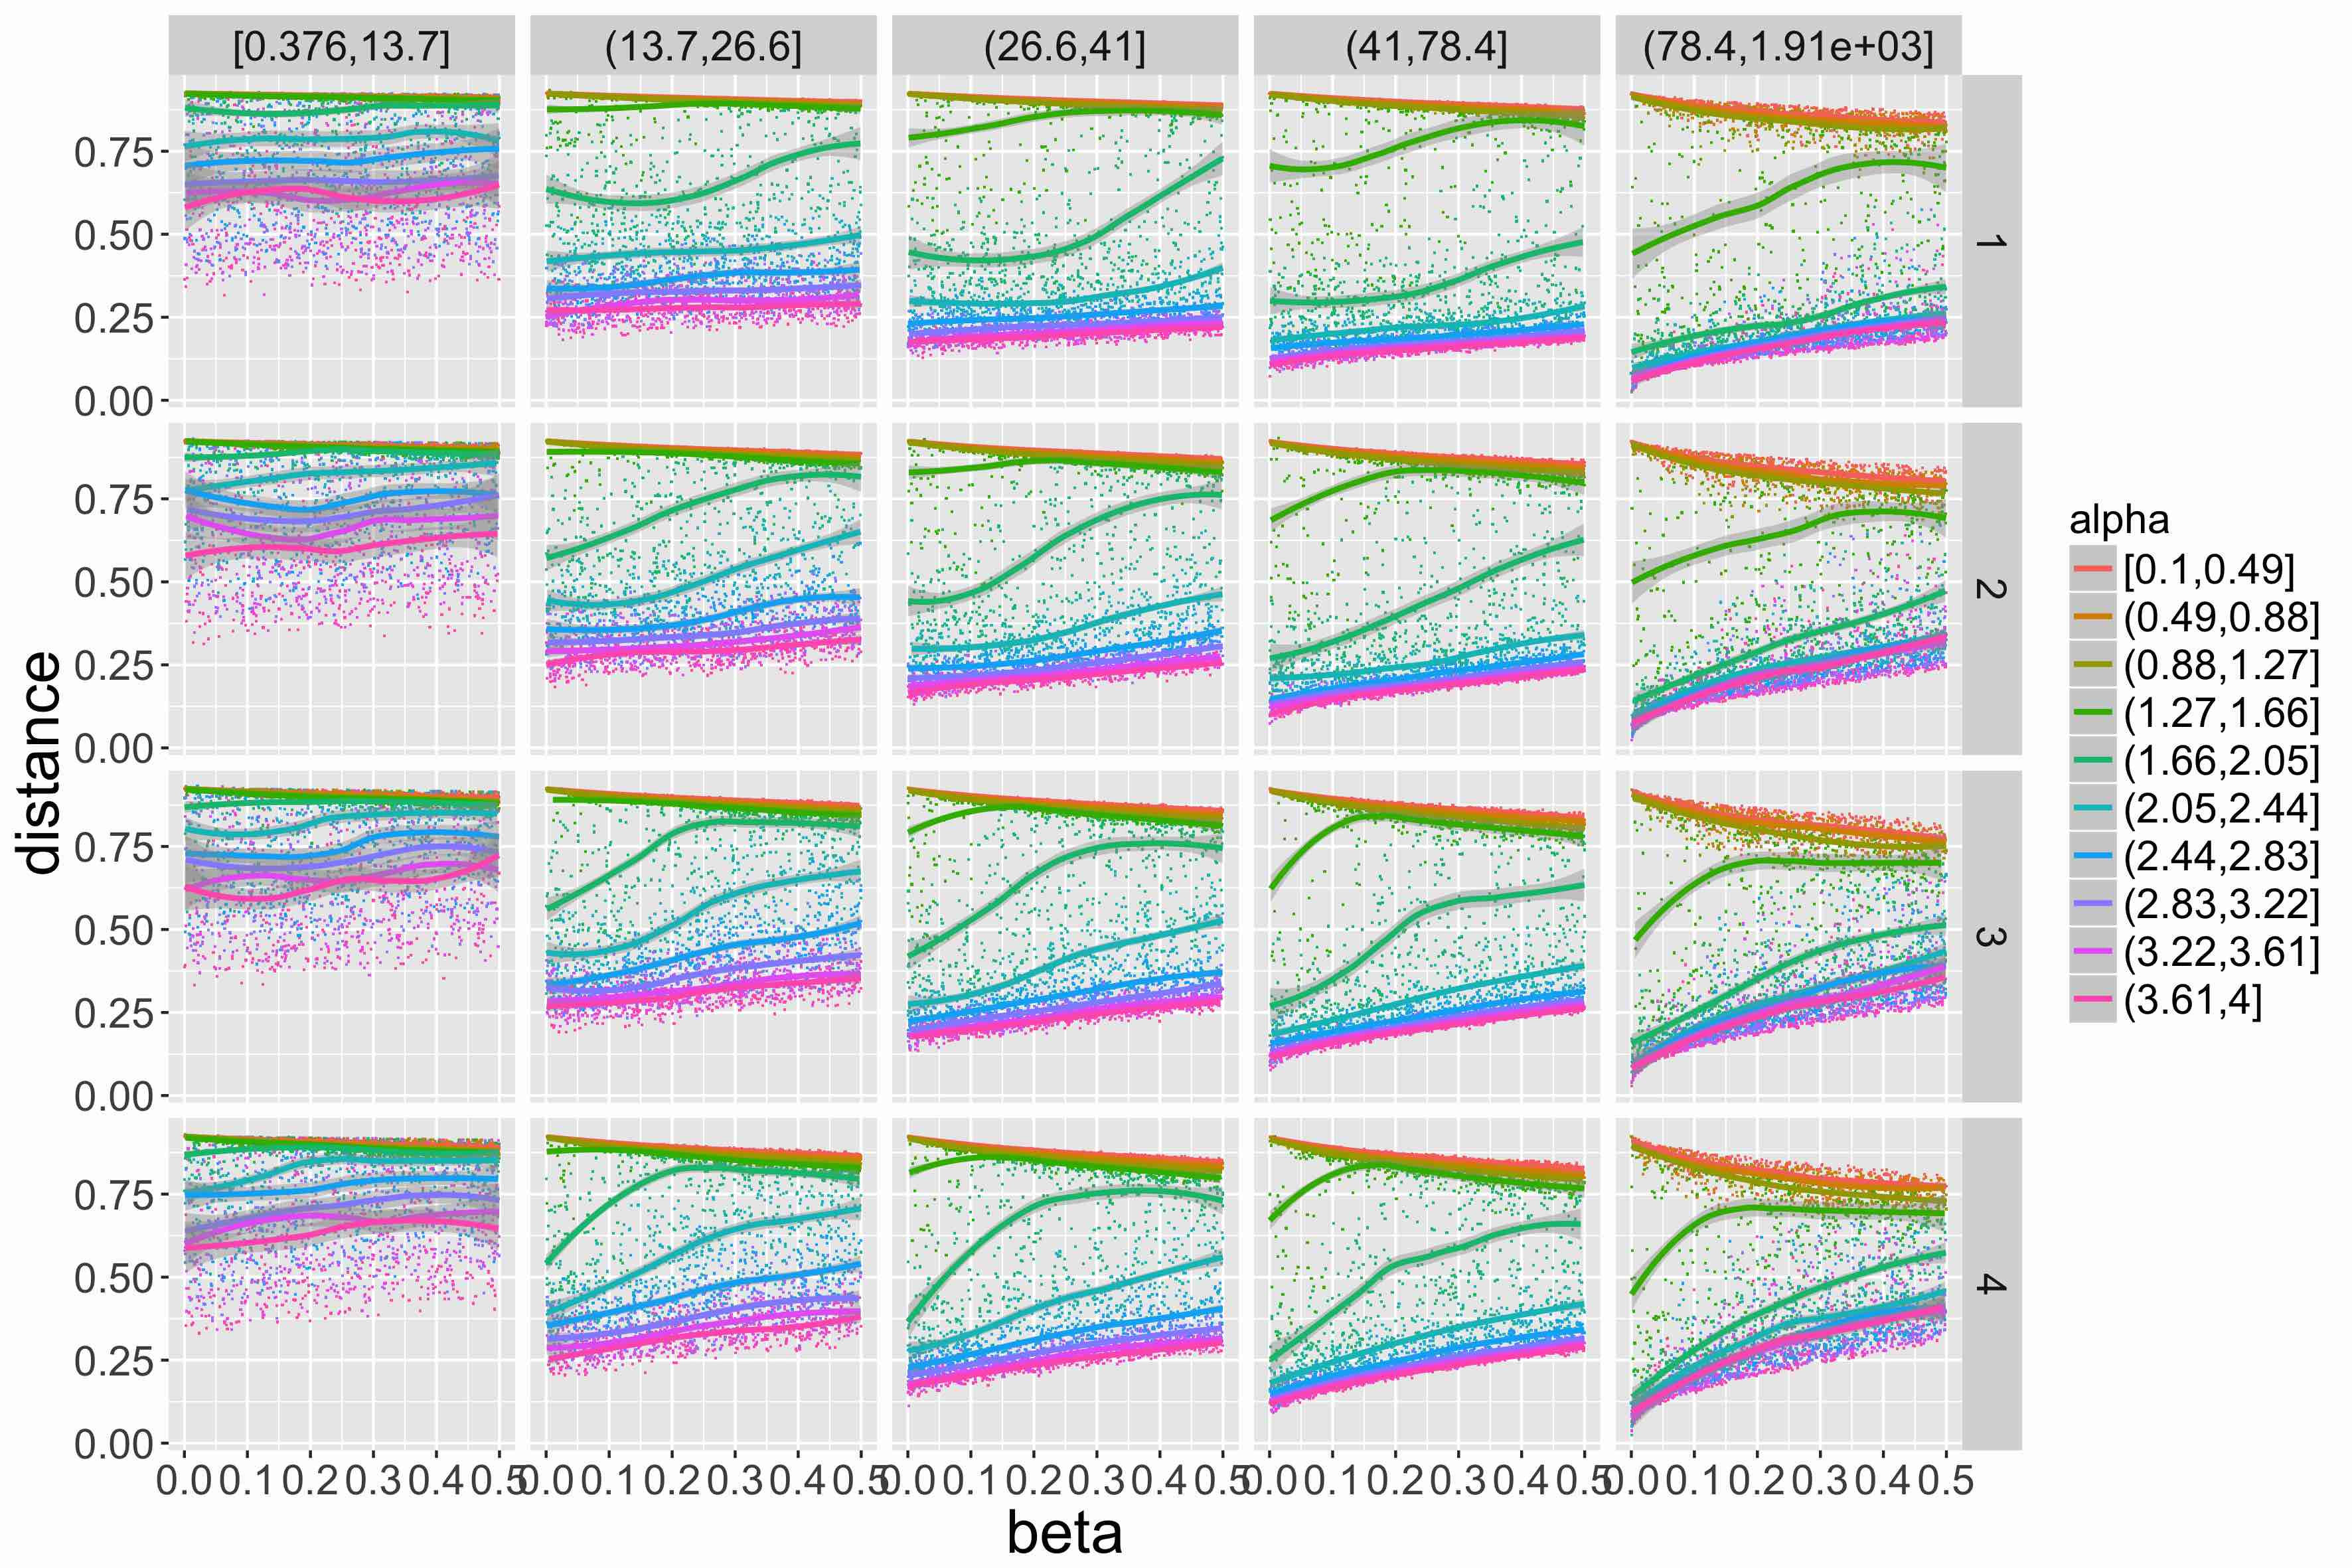
\includegraphics[width=0.8\textwidth]{Figures/Density/distance_beta}
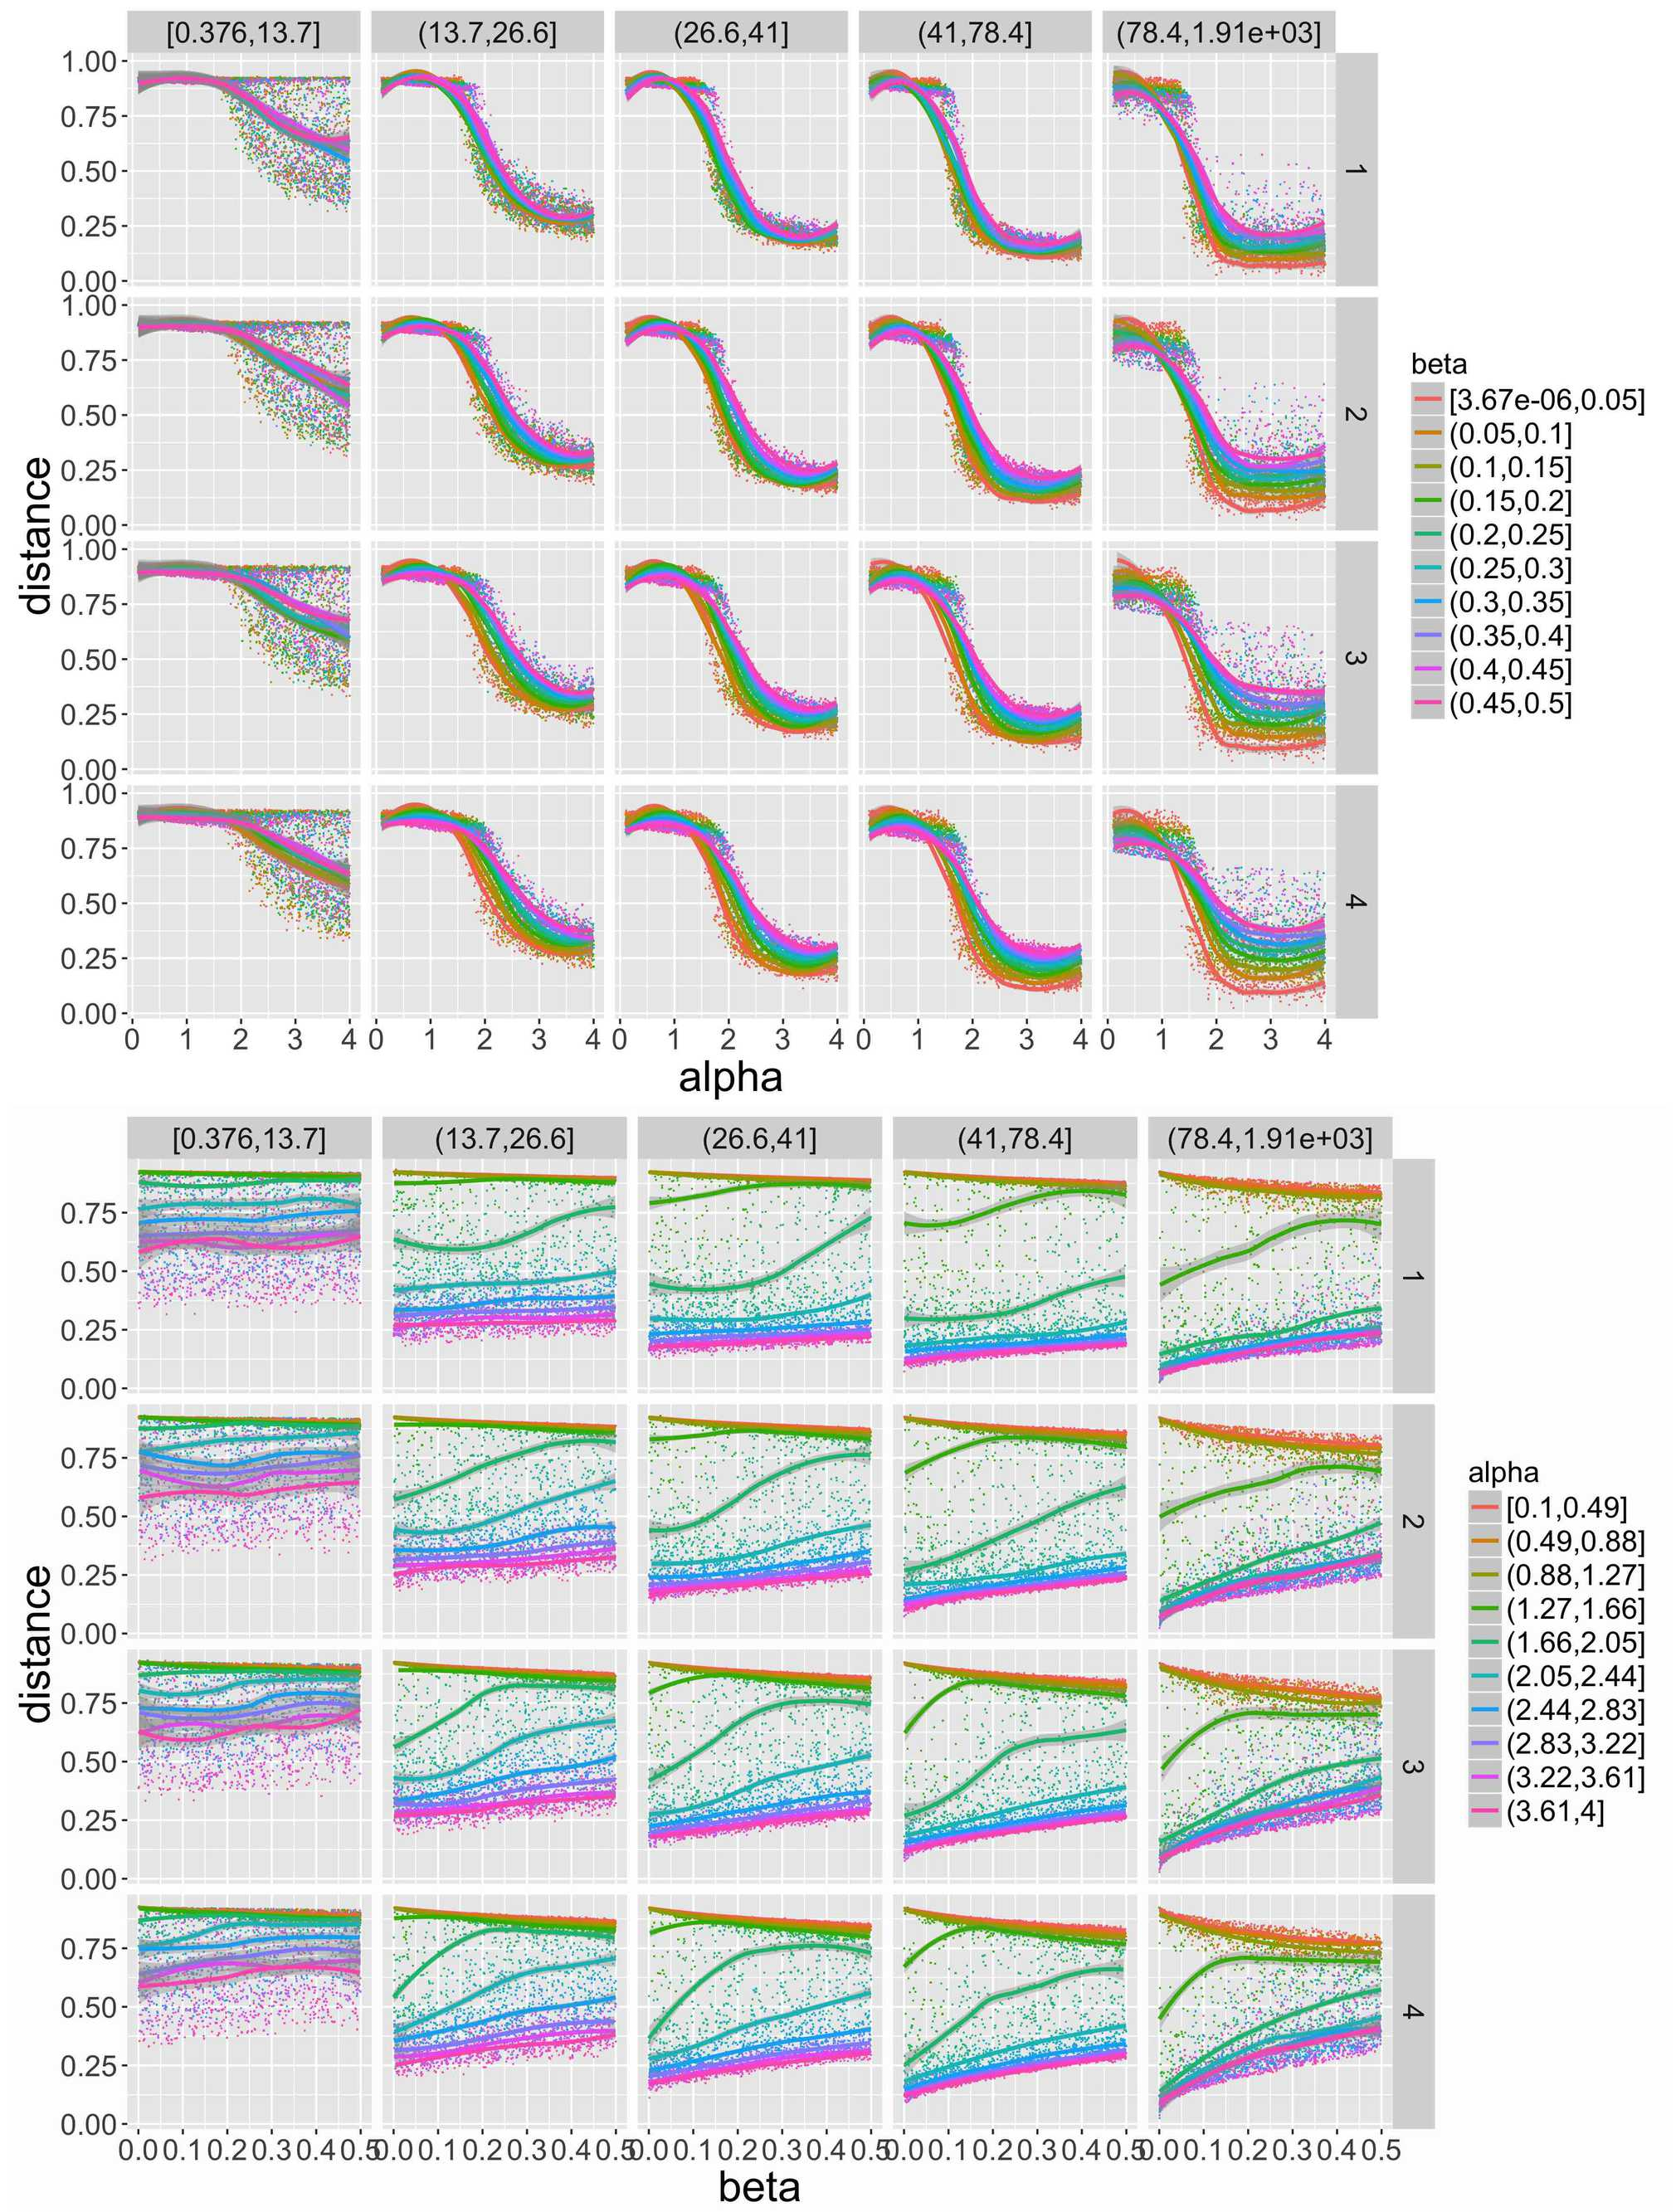
\includegraphics[width=\linewidth]{Figures/Final/A-density-distance.jpg}
\appcaption{Average distance index as a function of $\alpha$ (Top) and $\beta$ (Bottom) for varying $\beta$ (resp. $\alpha$) given by color, and varying $n_d$ (rows) and $N_G$ (columns).}{Distance moyenne en fonction de $\alpha$ (Haut) et $\beta$ (Bas) pour $\beta$ variable (resp. $\alpha$) donné par la couleur, et $n_d$ (lignes) et $N_G$ (colonnes) variables.\label{fig:app:density:distance}}
\end{figure}
%%%%%%%%%%%%%%%%%%%%


%%%%%%%%%%%%%%%%%%%%
\begin{figure}
%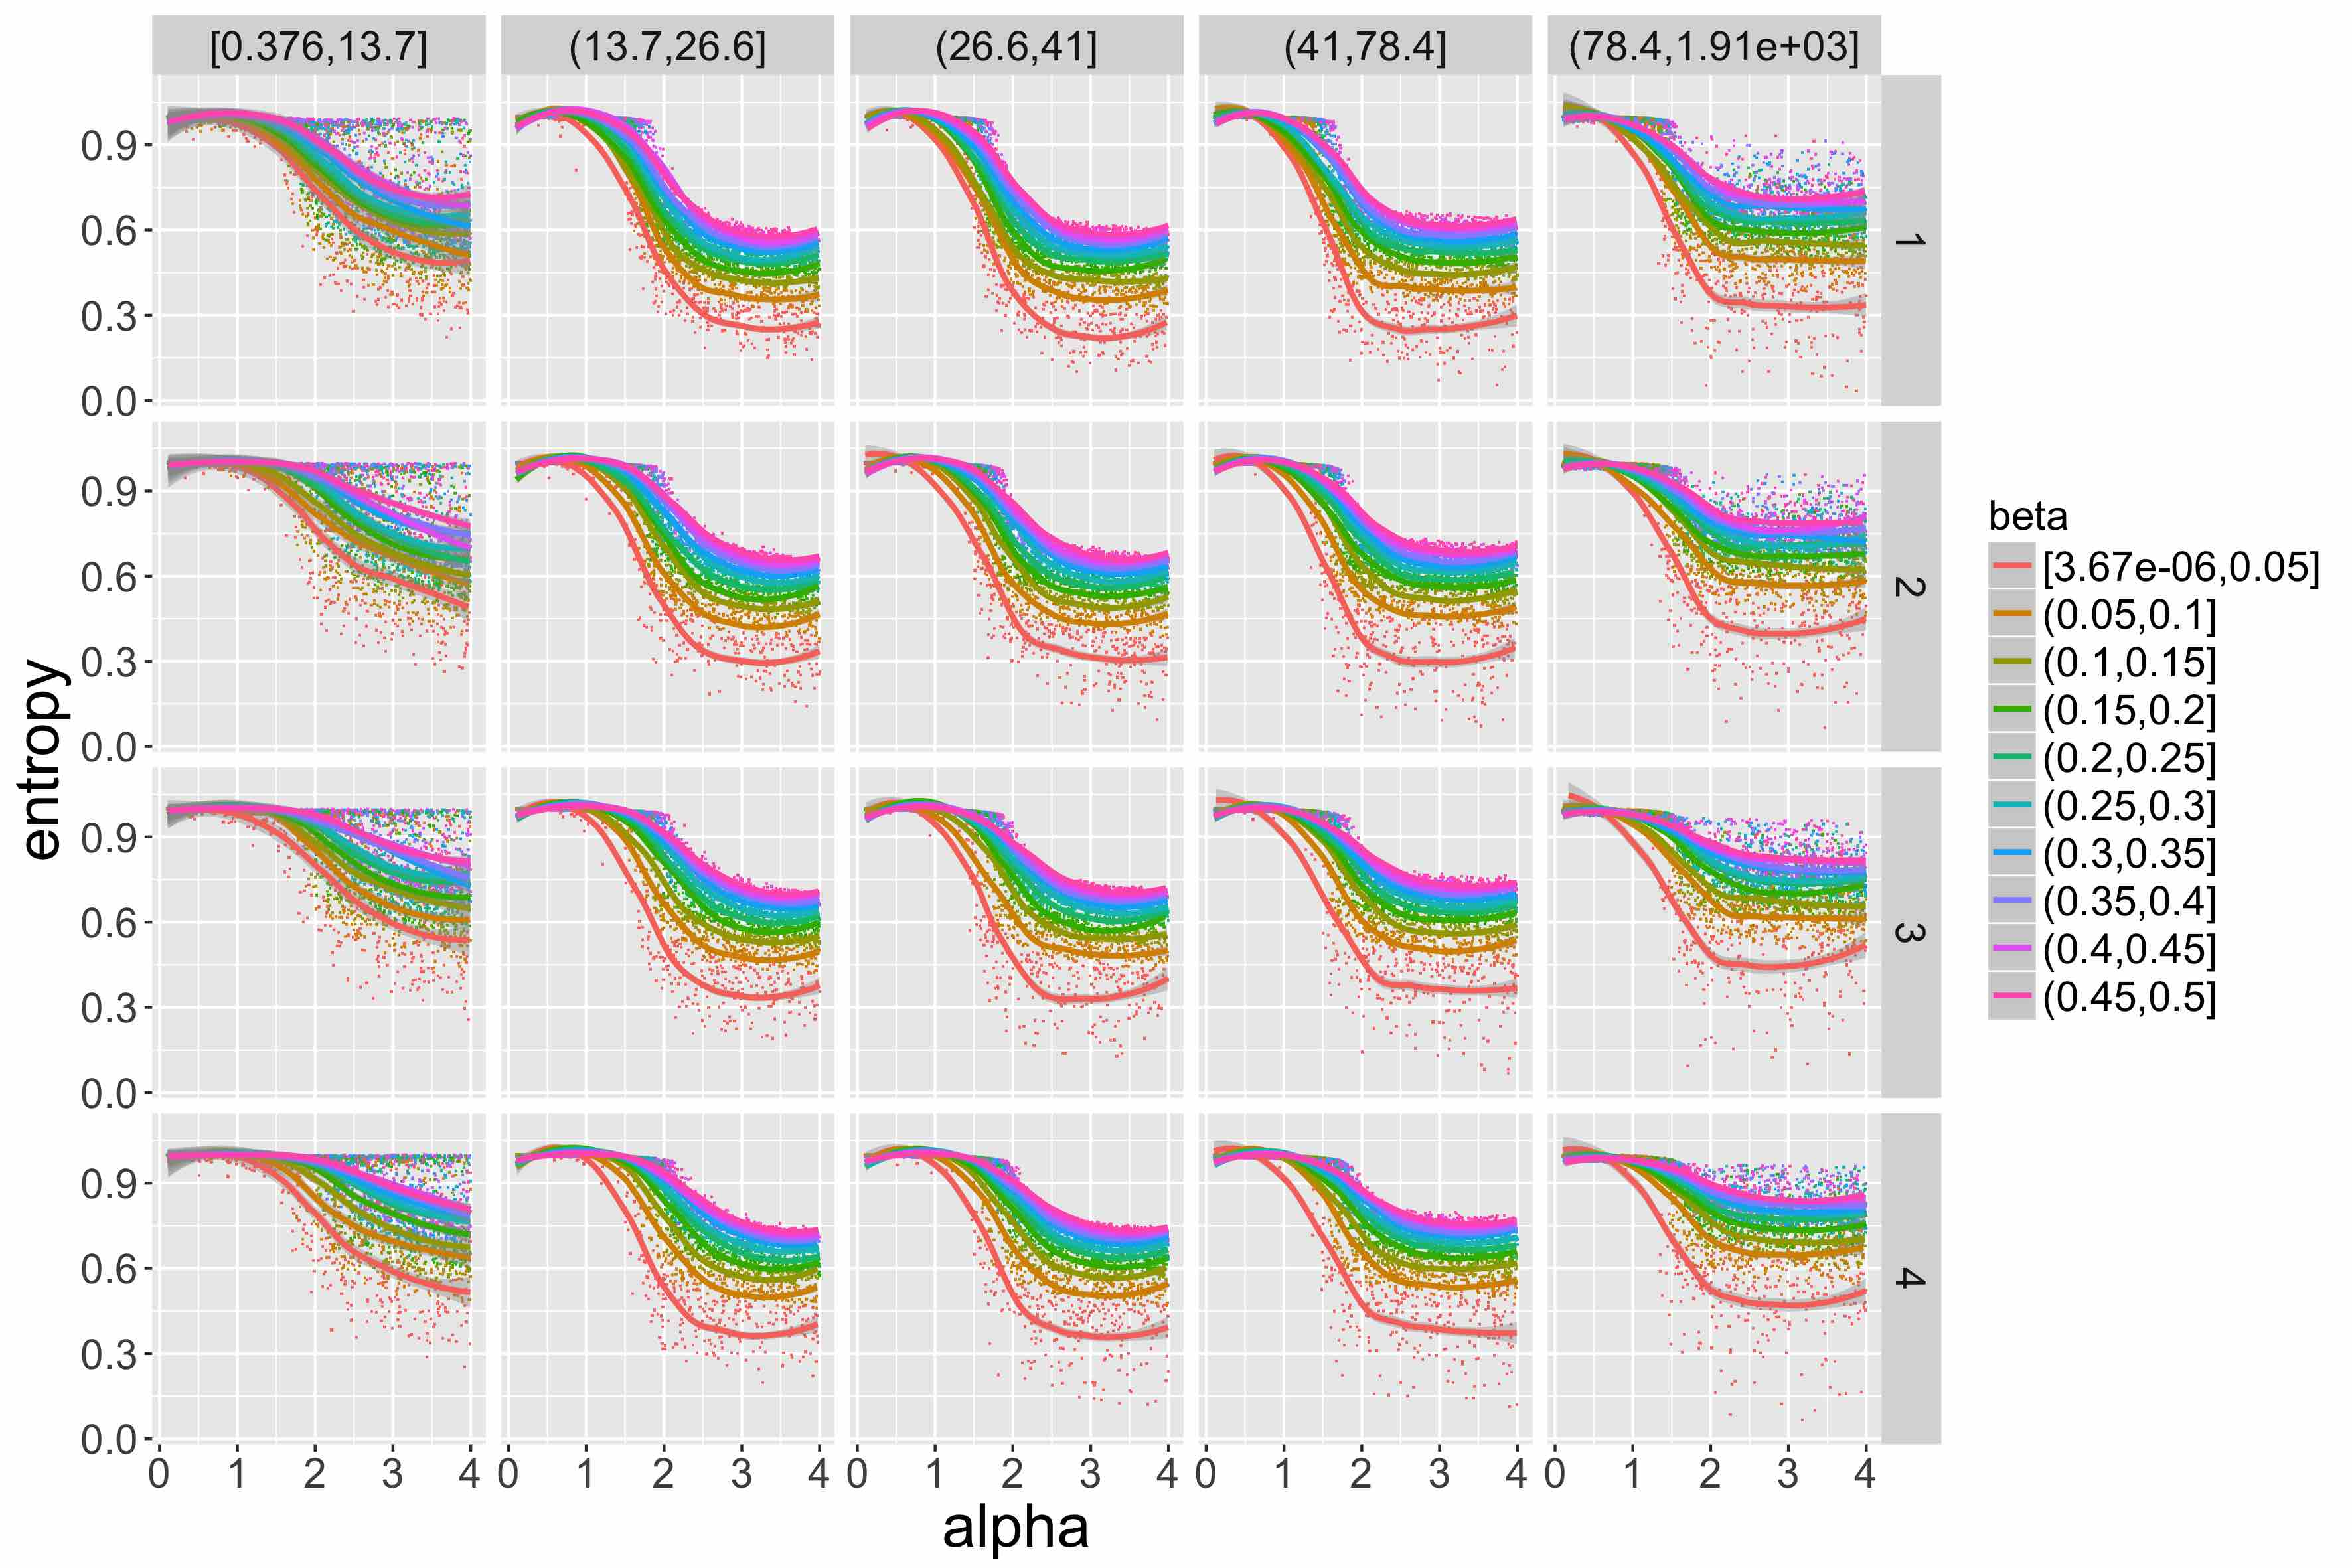
\includegraphics[width=0.8\textwidth]{Figures/Density/entropy_alpha}
%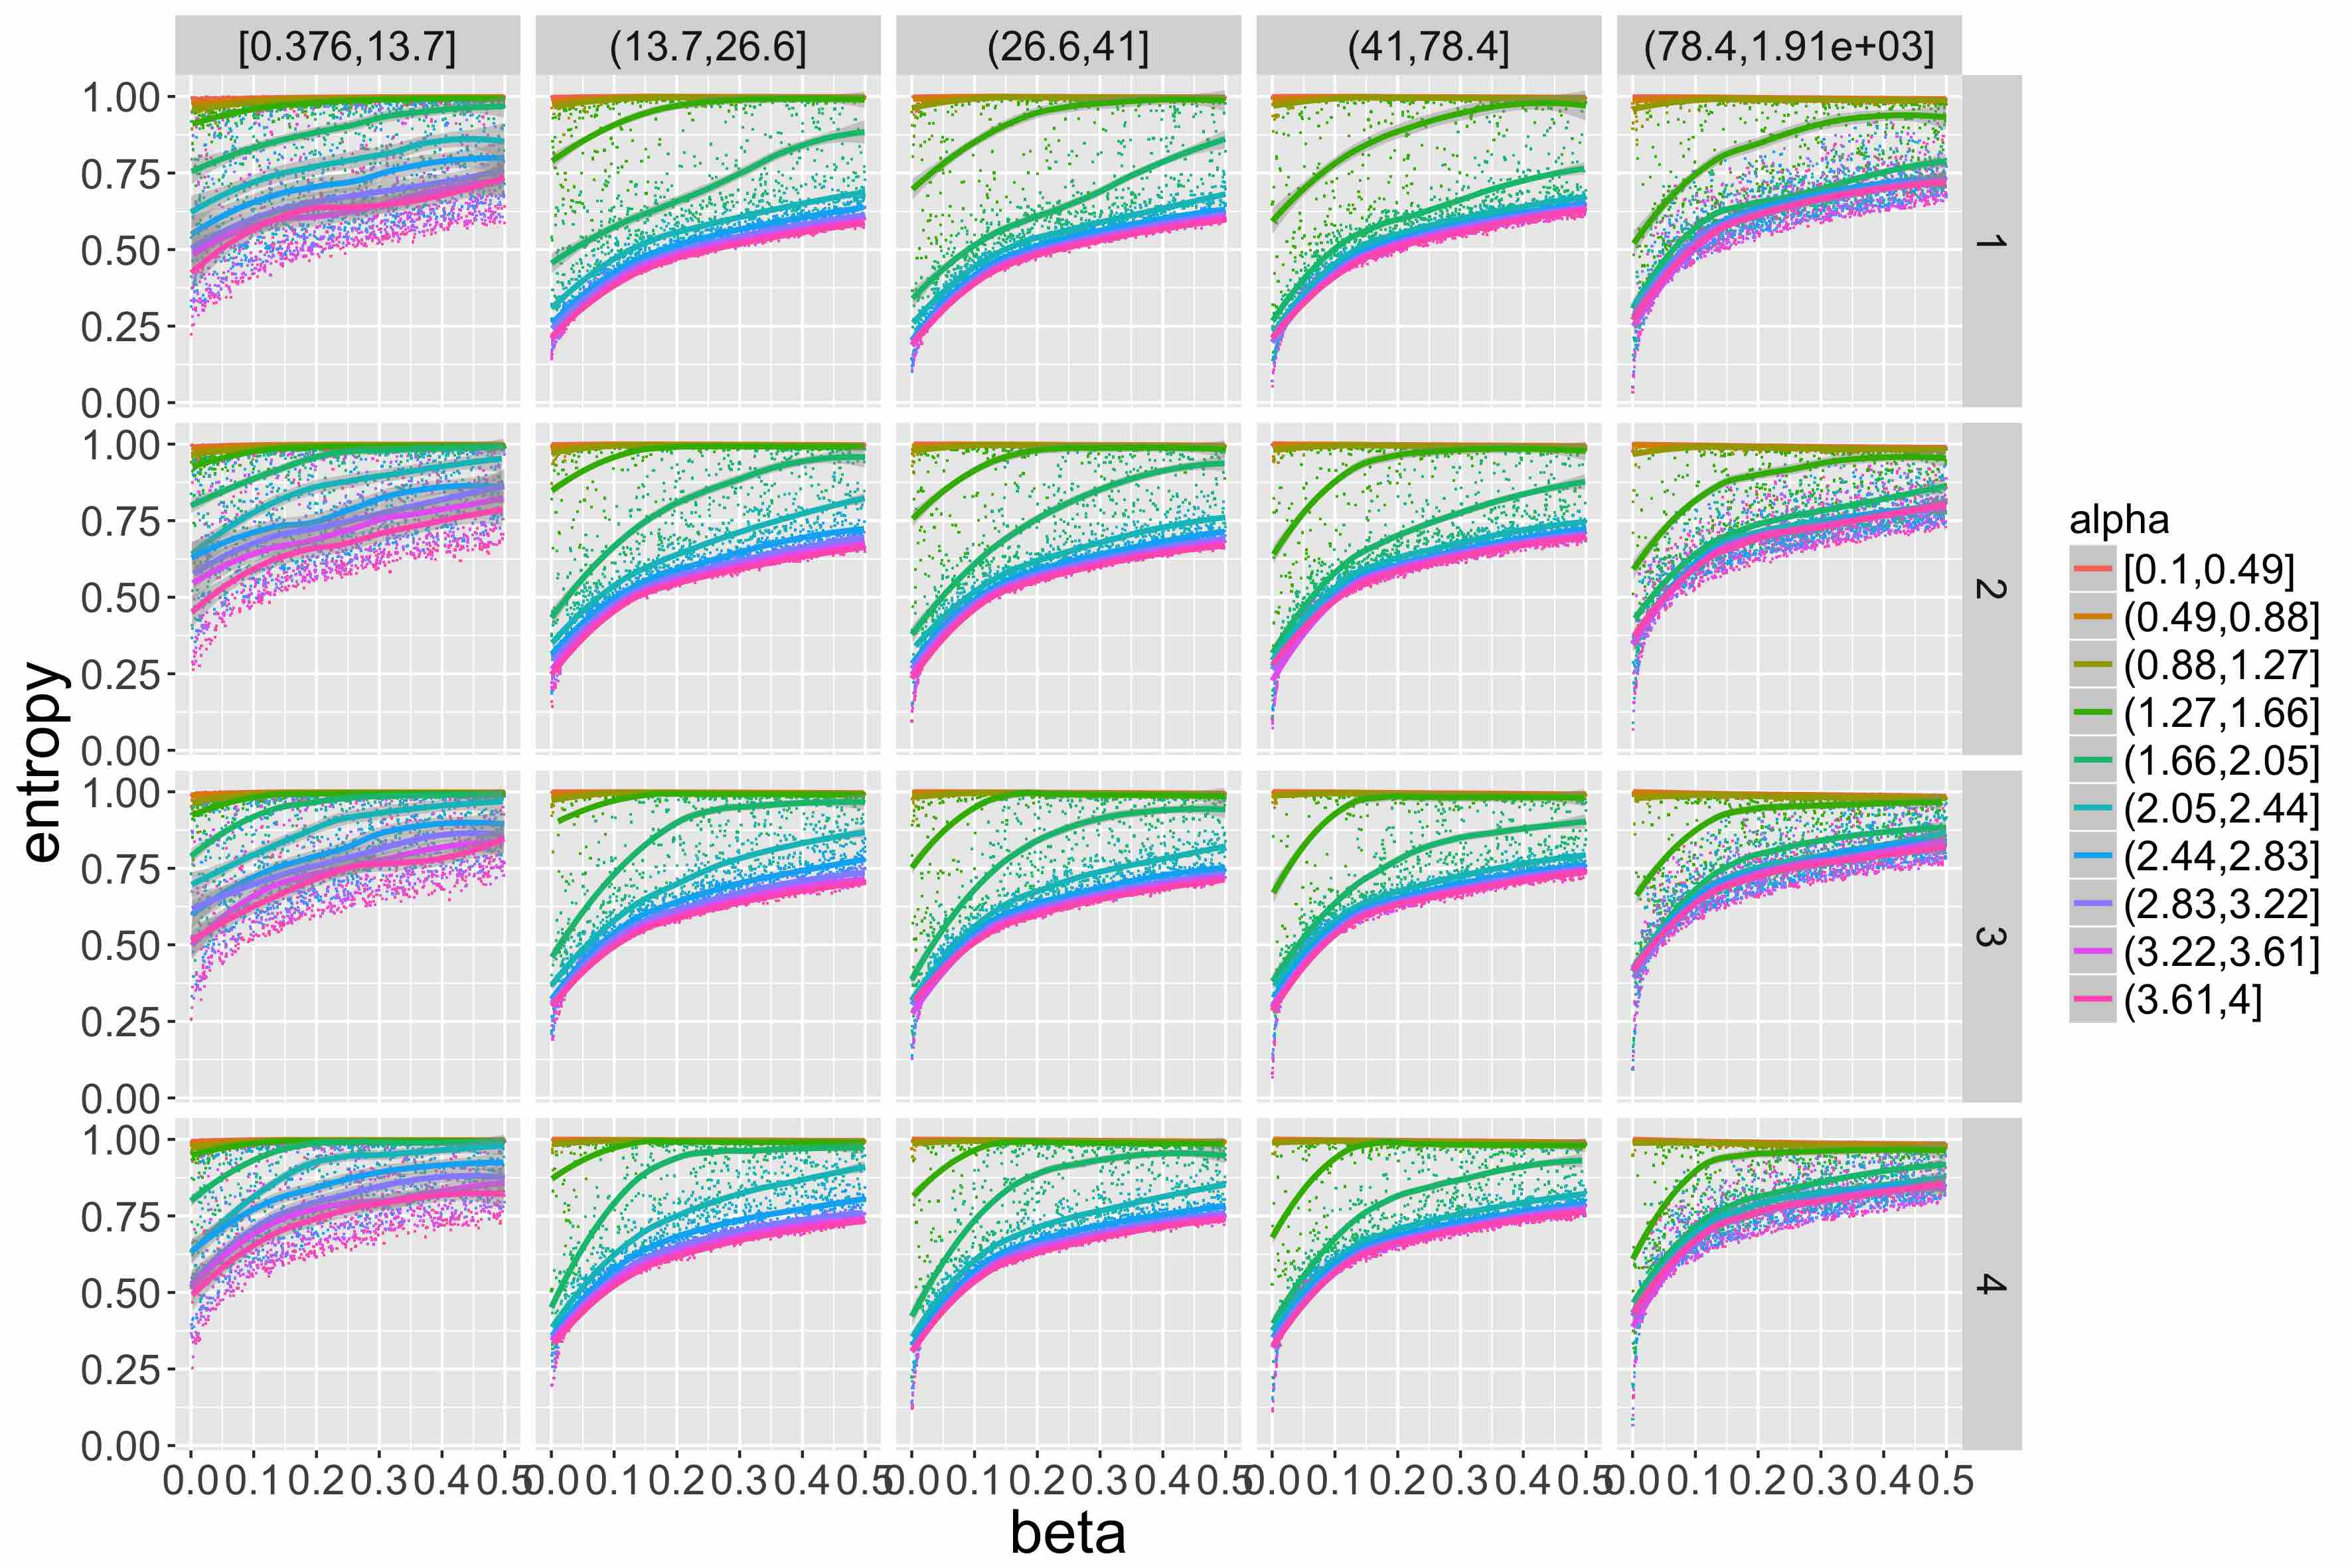
\includegraphics[width=0.8\textwidth]{Figures/Density/entropy_beta}
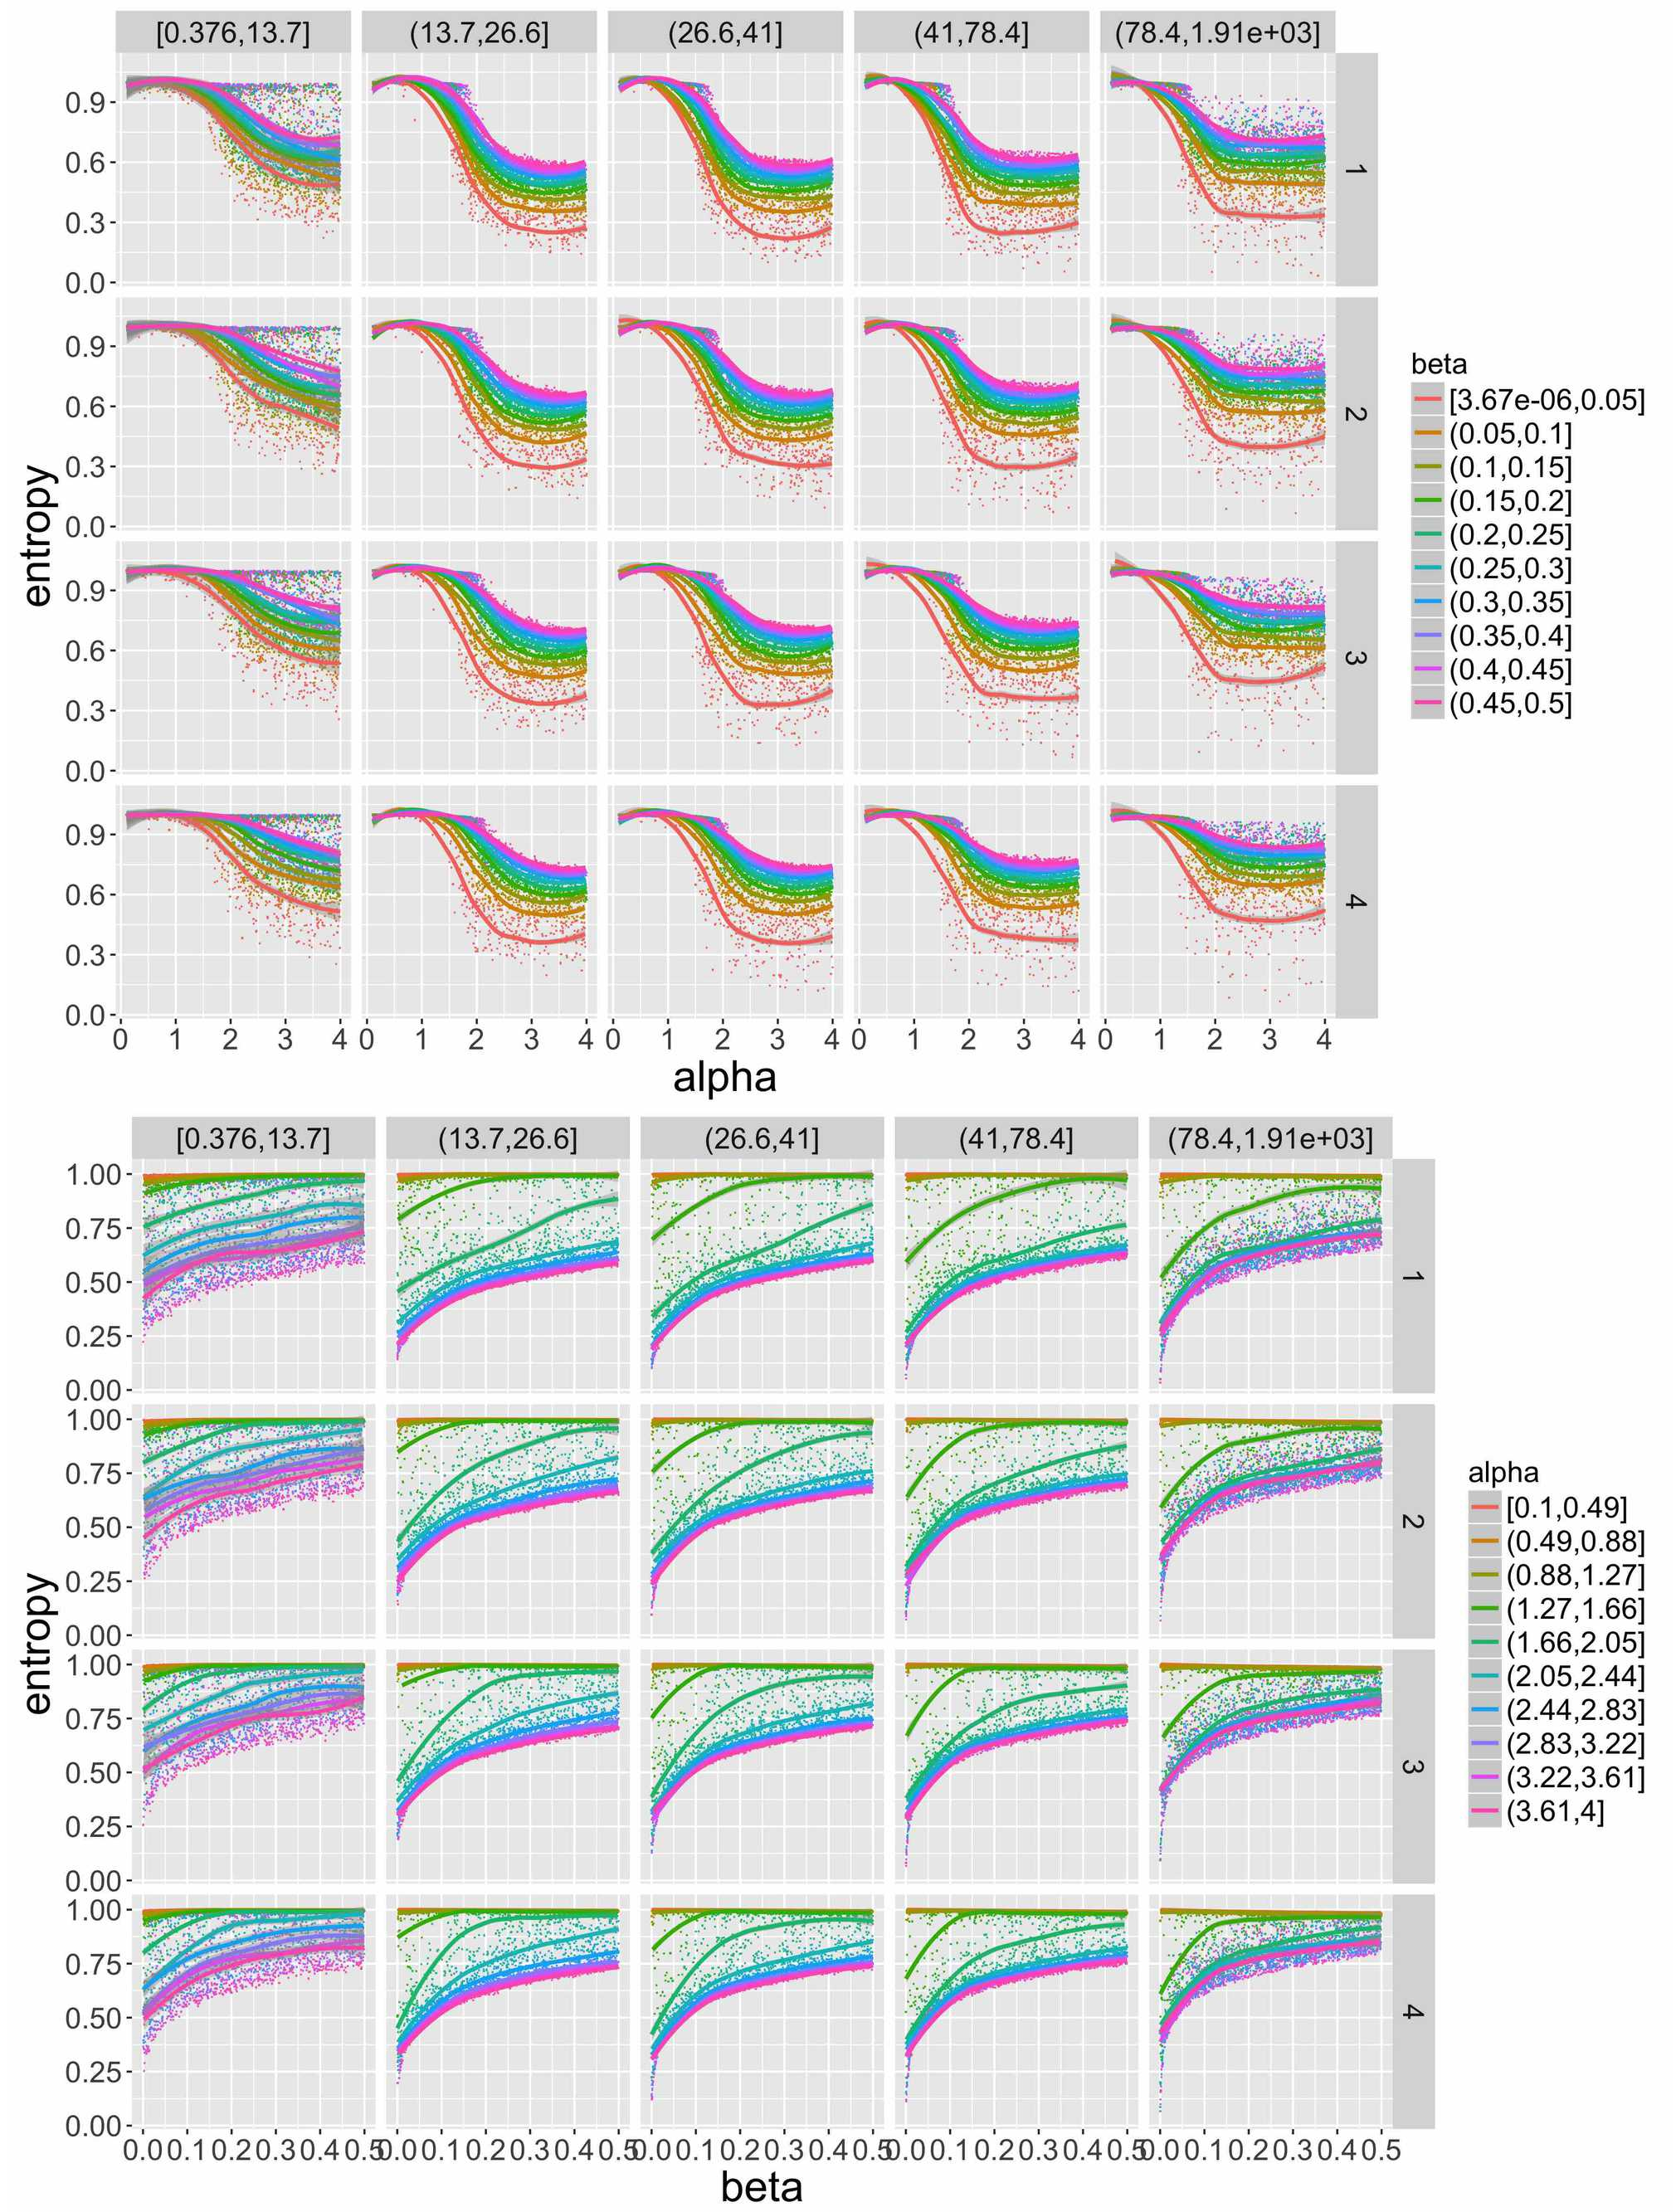
\includegraphics[width=\linewidth]{Figures/Final/A-density-entropy.jpg}
\appcaption{Entropy as a function of $\alpha$ (Top) and $\beta$ (Bottom) for varying $\beta$ (resp. $\alpha$) given by color, and varying $n_d$ (rows) and $N_G$ (columns).\label{fig:app:density:entropy}}{Entropie en fonction de $\alpha$ (Haut) et $\beta$ (Bas) pour $\beta$ variable (resp. $\alpha$) donné par la couleur, et $n_d$ (lignes) et $N_G$ (colonnes) variables.\label{fig:app:density:entropy}}
\end{figure}
%%%%%%%%%%%%%%%%%%%%






\subsubsection{Indicators Scatterplots}{Scatterplot des indicateurs}

% scatterplots - with real points

\bpar{
We show finally the full scatterplots of indicators, with real data points, in Fig.~\ref{fig:app:density:densityscatter}. These are preliminary step of the calibration on principal components, and we can see on these on which dimensions the model fails relatively to fit real data (in particular average distance).
}{
Nous montrons finalement les nuages de points complets des indicateurs, avec les points observés, en Fig.~\ref{fig:app:density:densityscatter}. Il s'agit de l'étape préliminaire à la calibration sur les composantes principales, et nous pouvons voir ici sur quelles dimensions le modèle échoue particulièrement à s'approcher des données observées (en particulier la distance moyenne).
}

%%%%%%%%%%%%%
\begin{figure}
%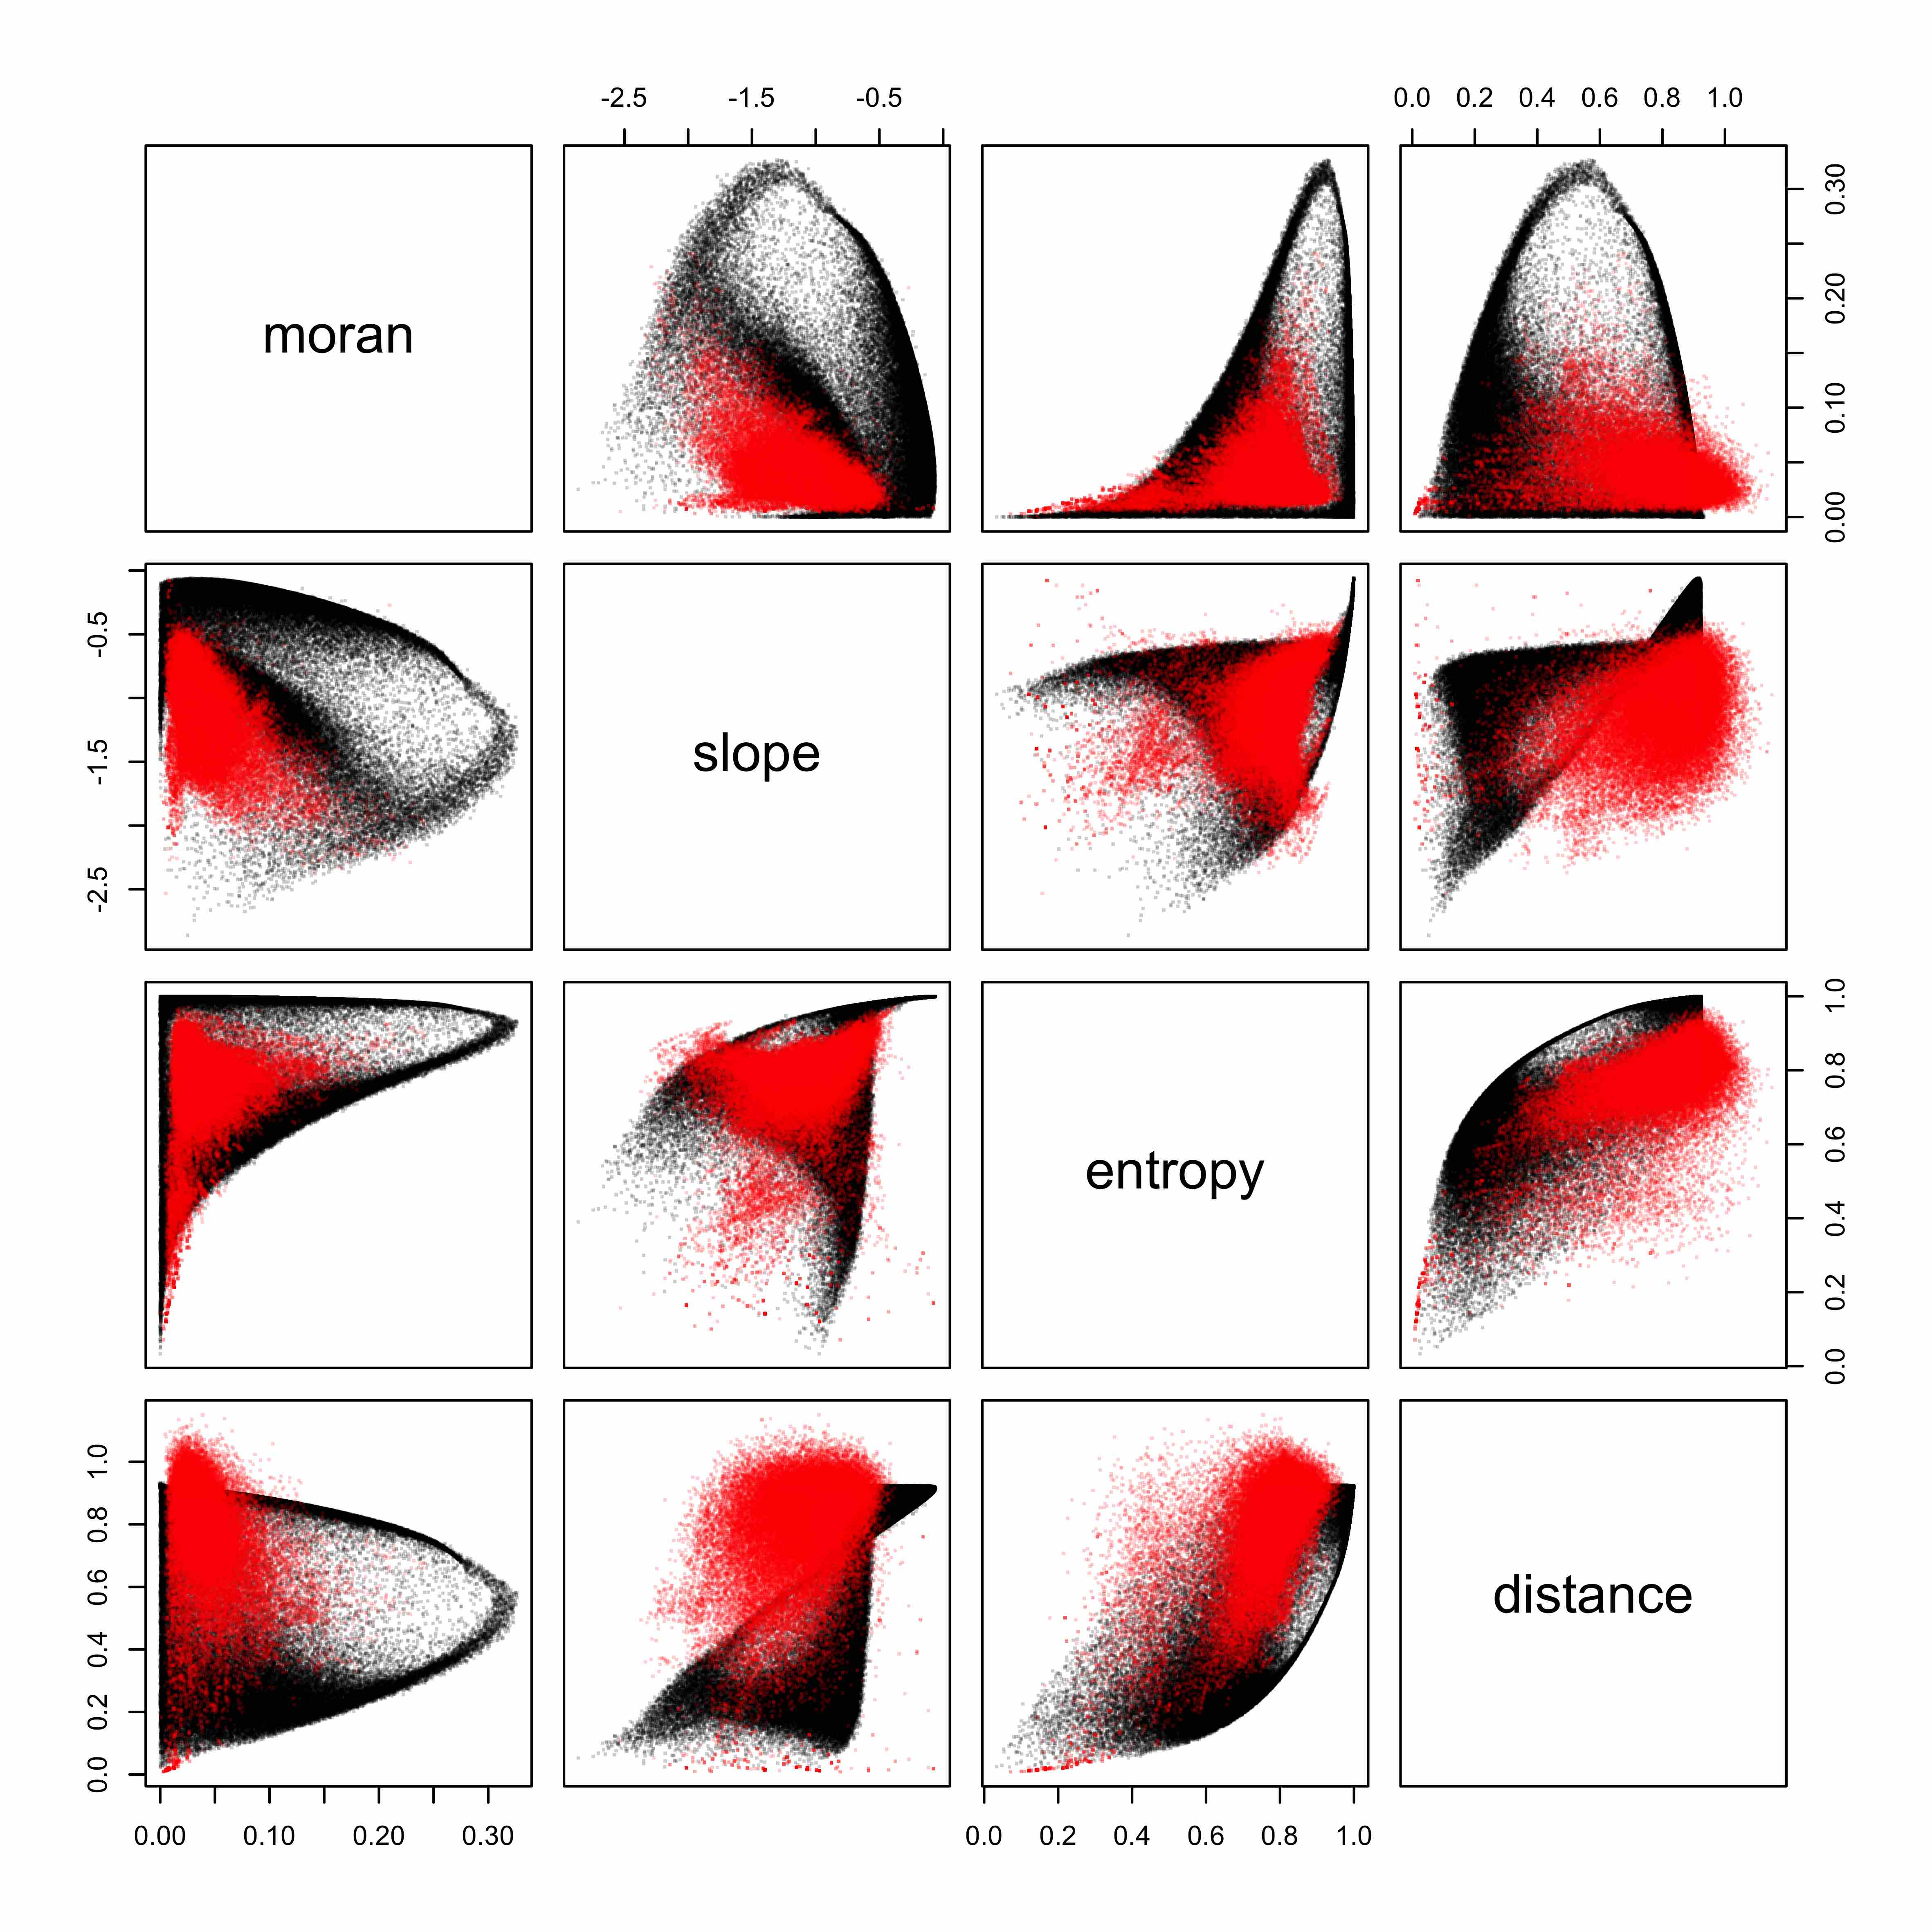
\includegraphics[width=\textwidth]{Figures/Density/scatter}
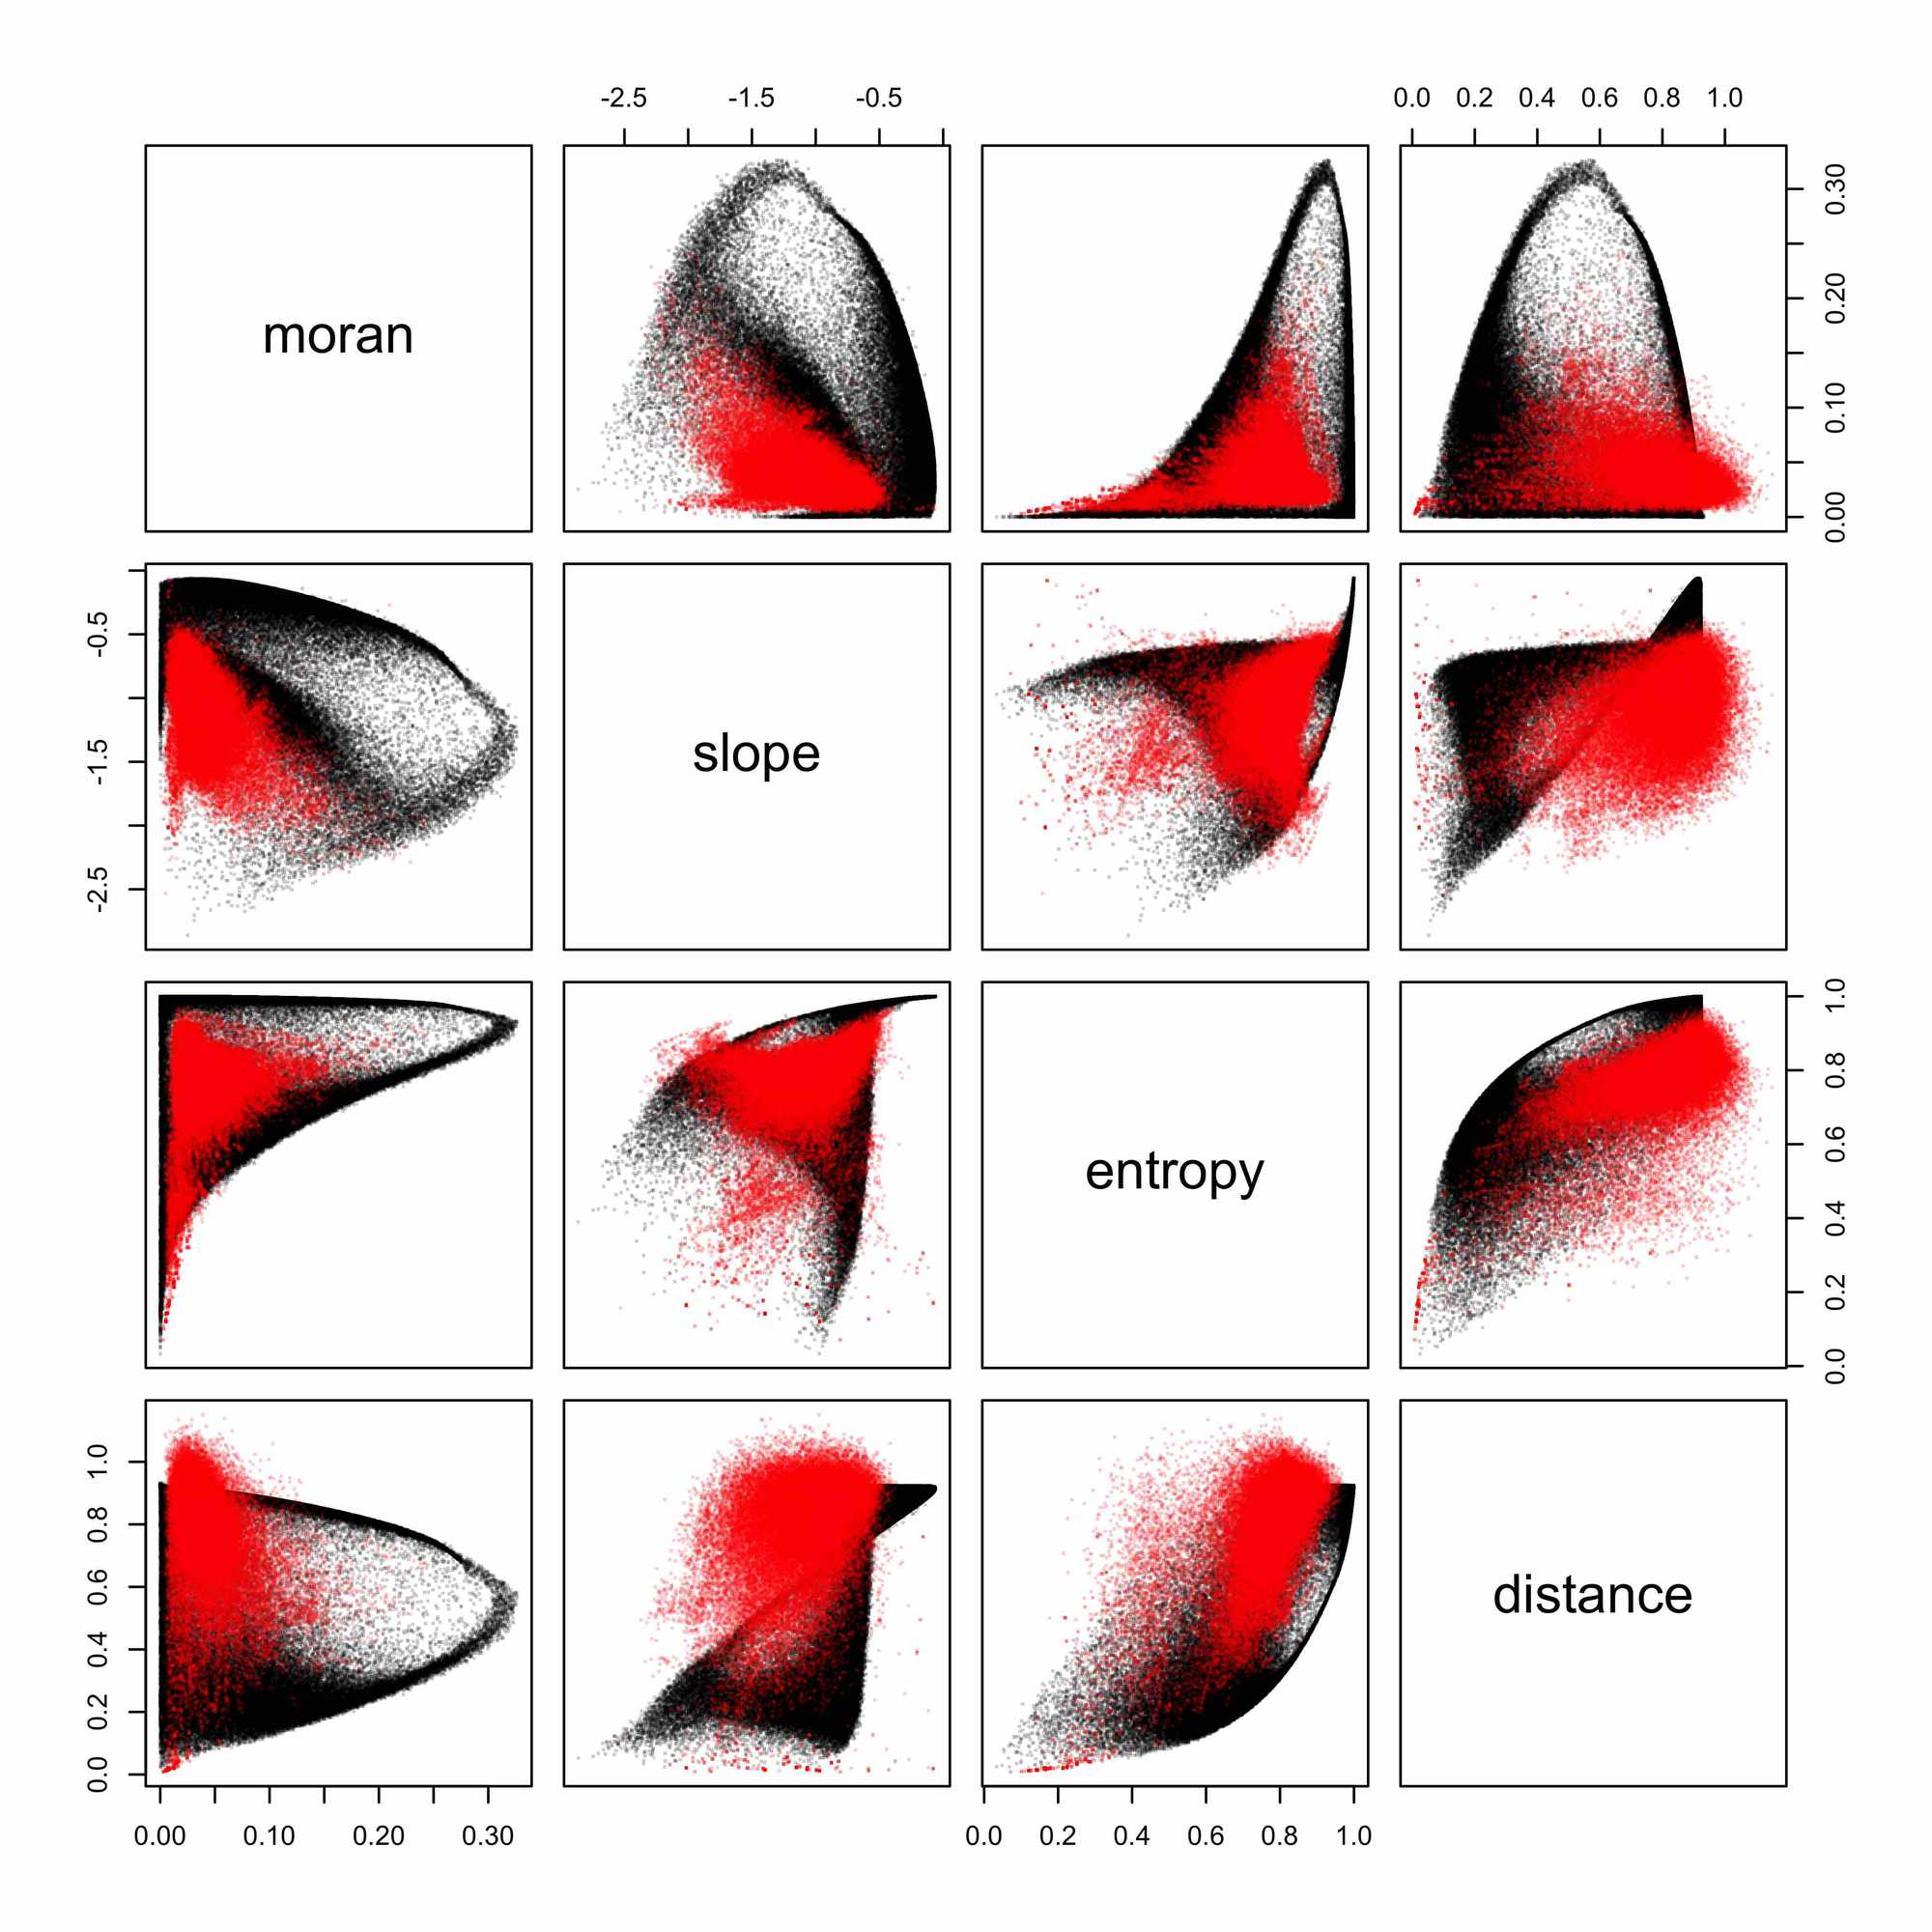
\includegraphics[width=\linewidth]{Figures/Final/A-density-densityscatter}
\appcaption{Scatterplots of indicators distribution in the sampled hypercube of the parameter space. Red points correspond to real data.\label{fig:app:density:densityscatter}}{Nuages de points des indicateurs dans l'hypercube échantillonné de l'espace des paramètres. Les points rouges correspondent aux données réelles.\label{fig:app:density:densityscatter}}
\end{figure}
%%%%%%%%%%%%%





\subsection{Semi-analytical analysis of the simplified model}{Analyse semi-analytique du modèle simplifié}


\subsubsection{Partial Differential Equation}{Equation aux dérivées partielles}


\bpar{
We propose to derive the PDE in a simplified setting. To recall the configuration given in main text, the system has one dimension, such that $x\in \mathbb{R}$ with $1/\delta x$ cells of size $\delta x$, and we use the expected values of cell population $p(x,t) = \Eb{P(x,t)}$. We furthermore take $n_d=1$. Larger values would imply derivatives at an order higher than 2 but the following results on the existence of a stationary solution should still hold. 
}{
Nous proposons de dériver l'EDP dans un cadre simplifié. Pour rappeler la configuration donnée en texte principal, le système a une dimension, tel que $x\in \mathbb{R}$ avec $1/\delta x$ cellules de taille $\delta x$, et nous utilisons les valeurs attendues des populations des cellules $p(x,t) = \Eb{P(x,t)}$. Nous prenons de plus $n_d=1$. Des valeurs plus grandes devraient impliquer des dérivées à un ordre supérieur à deux, mais les résultats qui suivent sur l'existence d'une solution stationnaire devraient être conservés.
}

\bpar{
Denoting $\tilde{p}(x,t)$ the intermediate populations obtained after the aggregation stage, we have
}{
En écrivant $\tilde{p}(x,t)$ les populations intermédiaires obtenues après l'étape d'agrégation, nous avons
}

\[
\tilde{p}(x,t) = p(x,t) + N_g\cdot \frac{p(x,t)^{\alpha}}{\sum_x p(x,t)^{\alpha}}
\]

\bpar{
since all populations units are added independently. If $\delta x \ll 1$ then $\sum_x p^{\alpha} \simeq \int_x p(x,t)^{\alpha}dx$ and we write this quantity $P_{\alpha}(t)$. We furthermore write $p=p(x,t)$ and $\tilde{p} = \tilde{p}(x,t)$ in the following for readability.
}{
puisque toutes les unités de population sont ajoutés indépendamment. Si $\delta x \ll 1$ alors $\sum_x p^{\alpha} \simeq \int_x p(x,t)^{\alpha}dx$ et nous écrivons cette quantité $P_{\alpha}(t)$. Nous notons de plus $p=p(x,t)$ et $\tilde{p} = \tilde{p}(x,t)$ par la suite pour faciliter la lecture.
}

\bpar{
The diffusion step is then deterministic, and for any cell not on the border ($0<x<1$), if $\delta t$ is the interval between two time steps, we have
}{
L'étape de diffusion est ensuite déterministe, et pour toute cellule qui n'est pas au bord ($0<x<1$), si $\delta t$ est l'intervalle entre deux pas de temps, nous avons
}


\[
\begin{split}
p(x,t+\delta t) & = (1 - \beta) \cdot \tilde{p} + \frac{\beta}{2} \left[\tilde{p}(x-\delta x,t) + \tilde{p}(x+\delta x,t)\right]\\
& = \tilde{p} + \frac{\beta}{2} \left[\left(\tilde{p}(x+\delta x,t) - \tilde{p}\right) - \left(\tilde{p} - \tilde{p}(x-\delta x,t)\right)\right]
\end{split}
\]

\bpar{
Assuming the partial derivatives exist, and as $\delta x \ll 1$, we make the approximation $\tilde{p}(x+\delta x,t) - \tilde{p} \simeq \delta x\cdot \frac{\partial \tilde{p}}{\partial{x}}(x,t)$, what gives 
}{
Sous l'hypothèse que les dérivées partielles existent, et comme $\delta x \ll 1$, nous faisons l'approximation $\tilde{p}(x+\delta x,t) - \tilde{p} \simeq \delta x\cdot \frac{\partial \tilde{p}}{\partial{x}}(x,t)$, ce qui donne
}


\[
\left(\tilde{p}(x+\delta x,t) - \tilde{p}\right) - \left(\tilde{p} - \tilde{p}(x-\delta x,t)\right) = \delta x \cdot \left(\frac{\partial \tilde{p}}{\partial{x}}(x,t) - \frac{\partial \tilde{p}}{\partial{x}}(x - \delta x,t)\right)
\]

\bpar{
and therefore at the second order
}{
et donc au second ordre
}


\[
p(x,t+\delta t) = \tilde{p} + \frac{\beta \delta x^2}{2} \cdot \frac{\partial^2 \tilde{p}}{\partial x^2}
\]

\bpar{
Substituting $\tilde{p}$ gives
}{
Le remplacement de $\tilde{p}$ donne
}


\[
\begin{split}
\frac{\partial^2 \tilde{p}}{\partial x^2} & = \frac{\partial^2 p}{\partial x^2} + \frac{N_G}{P_\alpha}\cdot \frac{\partial}{\partial x}\left[\alpha \frac{\partial p}{\partial x} p^{\alpha - 1}\right]\\
& = \frac{\partial^2 p}{\partial x^2} + \alpha \frac{N_G}{P_\alpha} \left[\frac{\partial^2 p}{\partial x^2} p^{\alpha - 1} + (\alpha - 1) \left( \frac{\partial p}{\partial x}\right)^2 p^{\alpha - 2}\right]
\end{split}
\]

\bpar{
By supposing that $\frac{\partial p}{\partial t}$ exists and that $\delta t$ is small, we have $p(x,t+\delta t) - p(x,t) \simeq \delta t\frac{\partial p}{\partial t}$, what finally yields , by combining the results above, the partial differential equation
}{
En supposant que $\frac{\partial p}{\partial t}$ existe et que $\delta t$ est petit, nous avons $p(x,t+\delta t) - p(x,t) \simeq \delta t\frac{\partial p}{\partial t}$, ce qui donne finalement, par combinaison des résultats ci-dessus, l'équation aux dérivées partielles
}


\begin{equation}\label{eq:pde}
\delta t \cdot \frac{\partial p}{\partial t} = \frac{N_G \cdot p^{\alpha}}{P_{\alpha}(t)} + \frac{\alpha \beta (\alpha - 1) \delta x^2}{2}\cdot \frac{N_G \cdot p^{\alpha-2}}{P_{\alpha}(t)} \cdot \left(\frac{\partial p}{\partial x}\right)^2 + \frac{\beta \delta x^2}{2} \cdot \frac{\partial^2 p}{\partial x^2} \cdot\left[ 1 + \alpha \frac{N_G p^{\alpha - 1}}{P_{\alpha(t)}} \right]
\end{equation}


\bpar{
Initial conditions should be specified as $p_0(x) = p(x,t_0)$. To have a well-posed problem similar to more classical PDE problems, we need to assume a domain and boundary conditions. A finite support is expressed by $p(x,t)=0$ for all $t$ and $x$ such that $\left|x\right|>x_m$.
}{
Les conditions initiales sont spécifiées par $p_0(x) = p(x,t_0)$. Pour obtenir un problème bien posé comme dans des formulations PDE plus classiques, nous devons supposer un domaine et des conditions au bord. Un support fini est traduit par $p(x,t)=0$ pour tout $t$ et $x$ tel que $\left|x\right|>x_m$.
}


%An infinite domain implies that density, in the sense of population proportion $d(x,t) = \frac{p(x,t)}{P_1(t)}$, goes to zero anywhere when time goes to infinity. Indeed, $P_1(t)=N_G\cdot t$. If $d(x,t)$ does not vanish, there exist $t_1$ such that  -> not that simple indeed


\subsubsection{Stationary solution for density}{Solution stationnaire pour la densité}


\bpar{
The non-linearity and the integral terms making the equation above out of the scope for analytical resolution, we study its behavior numerically in some cases. Taking a simple initial condition $p_0(0)=1$ and $p_0(x)=0$ for $x\neq 0$, we show that on a finite domain, density $d(x,t)$ always converge to a stationary solution for large $t$, for a large set of values of $(\alpha,\beta)$ with fixed $N_G=10$ ($\alpha\in \left[0.4,1.5\right]$ varying with step $0.025$ and $\log\beta \in \left[-1,-0.5\right]$ with step $0.1$). We show in Fig.~\ref{fig:app:density:stationary} the corresponding trajectories on a typical subset. The variation of the asymptotic distribution as a function of $\alpha$ and $\beta$ are not directly visible, as they depend on very low values of the outward flows at boundaries. We give in Fig.~\ref{fig:app:density:pmax} their behavior, by showing the value of the maximum of the distribution. Low values of $\beta$ give an inversion in the effect of $\alpha$, whereas high values of $\beta$ give comparable values for all $\alpha$.
}{
La non-linéarité et les termes intégraux rendant l'équation ci-dessus hors d'atteinte d'une résolution analytique, nous étudions son comportement de manière numérique pour certaines configurations. Prenant une condition initiale simple $p_0(0)=1$ et $p_0(x)=0$ pour $x\neq 0$, nous montrons que sur un domaine fini, la densité $d(x,t)$ converge toujours vers une solution stationnaire pour les grandes valeurs de $t$, pour un grand nombre de valeurs pour $(\alpha,\beta)$ avec $N_G=10$ fixé ($\alpha\in \left[0.4,1.5\right]$ variant avec un pas de $0.025$ et $\log\beta \in \left[-1,-0.5\right]$ avec un pas de $0.1$). Nous montrons en Fig.~\ref{fig:app:density:stationary} les trajectoires correspondantes sur un sous-ensemble typique. La variation des distributions asymptotiques comme fonction de $\alpha$ et $\beta$ ne sont pas directement observables, puisqu'elle dépendent des valeurs très faibles des flux sortants aux bords. Nous donnons en Fig.~\ref{fig:app:density:pmax} leur comportement, en donnant la valeur du maximum de la distribution. Les valeurs faibles de $\beta$ mènent à une inversion de l'effet de $\alpha$, tandis que les fortes valeurs de $\beta$ donnent des valeurs comparables pour tous les $\alpha$.
}



%%%%%%%%%%%%%%%%%%%%
\begin{figure}[h!]
%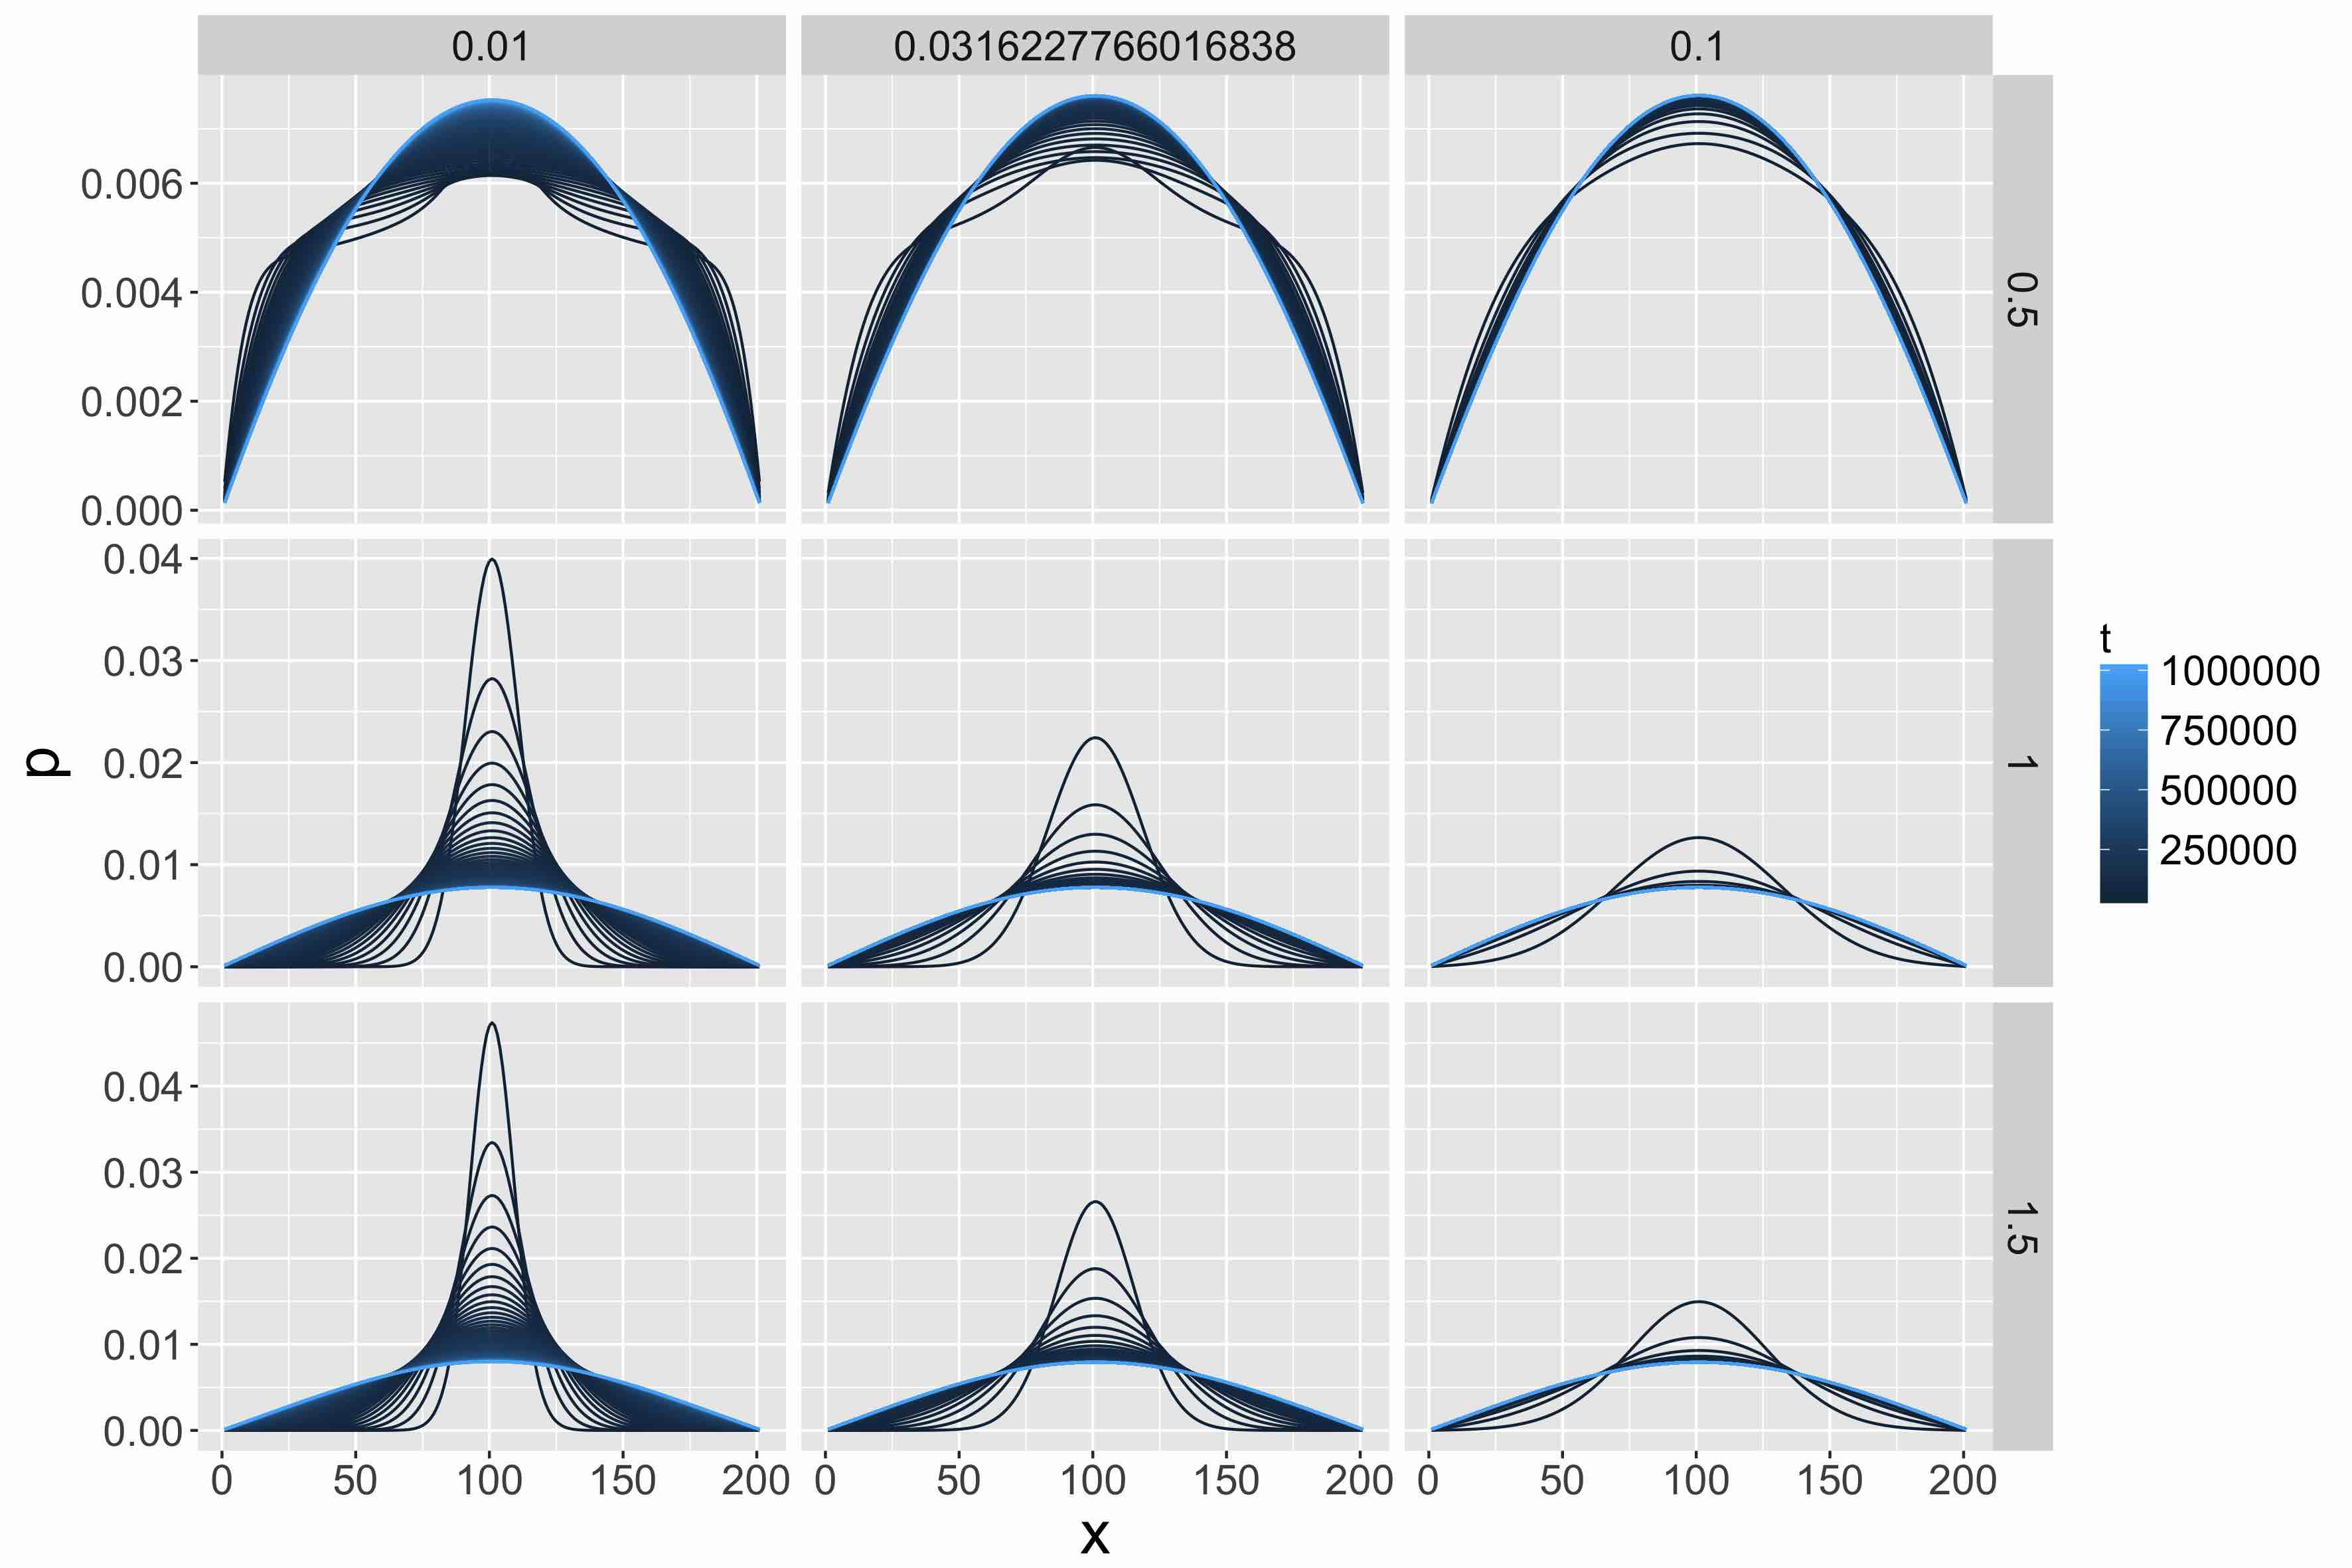
\includegraphics[width=\textwidth]{Figures/Density/stationary}
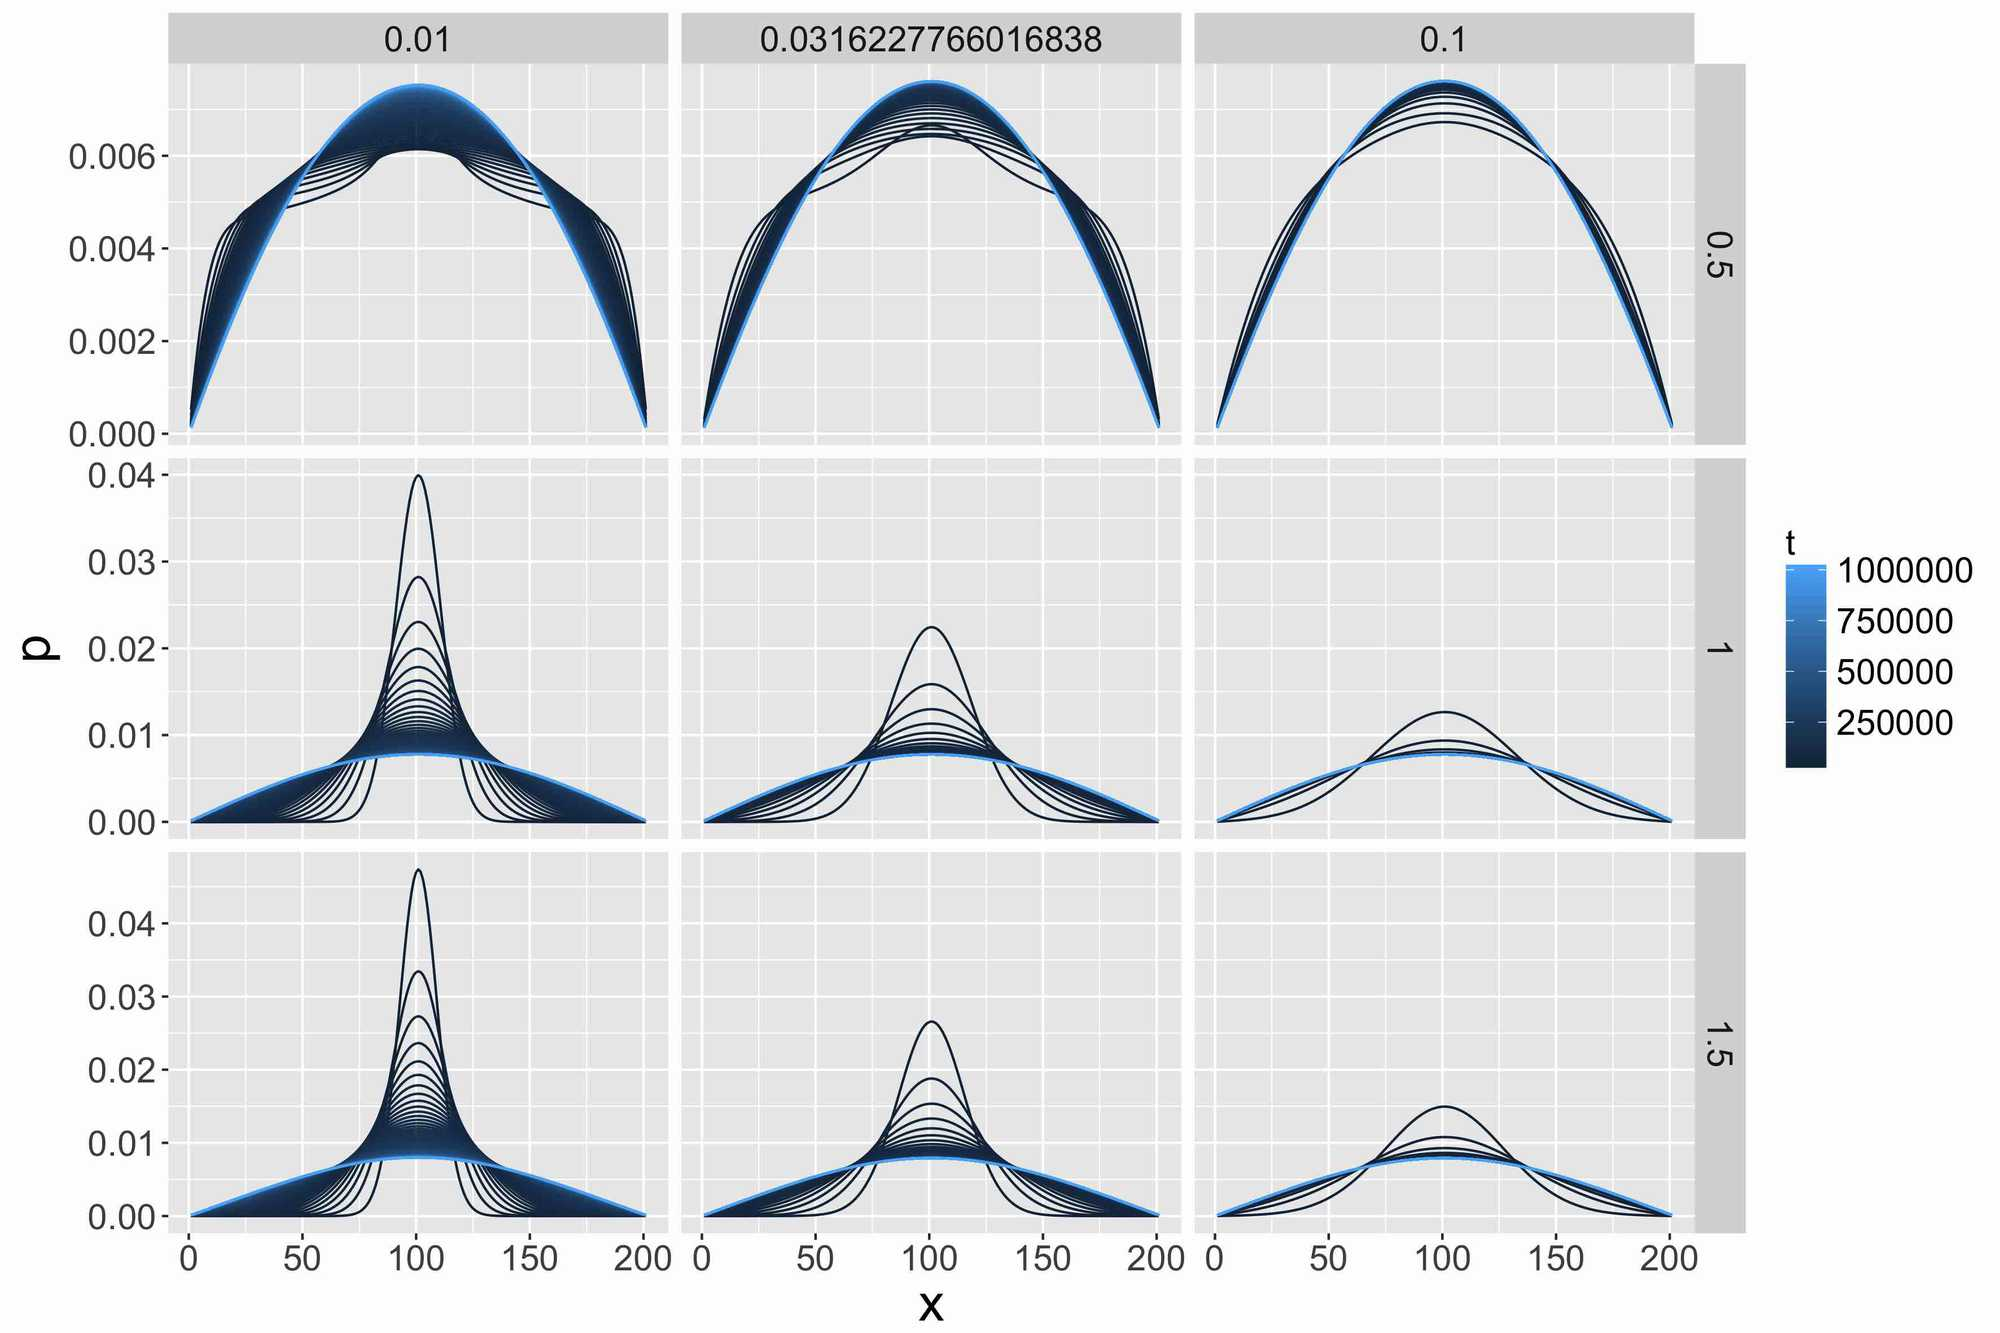
\includegraphics[width=\linewidth]{Figures/Final/A-density-stationary.jpg}
\appcaption{Trajectories of densities as a function of the spatial dimension, for varying $\beta$ (columns) and $\alpha$ (rows). Color gives time.\label{fig:app:density:stationary}}{Trajectoires des densités en fonction de la coordonnée spatiale, pour $\beta$ variable (colonnes) et $\alpha$ variable (lignes). Le niveau de couleur donne le temps.\label{fig:app:density:stationary}}
\end{figure}
%%%%%%%%%%%%%%%%%%%%



%%%%%%%%%%%%%%%%%%%%
\begin{figure}[h!]
%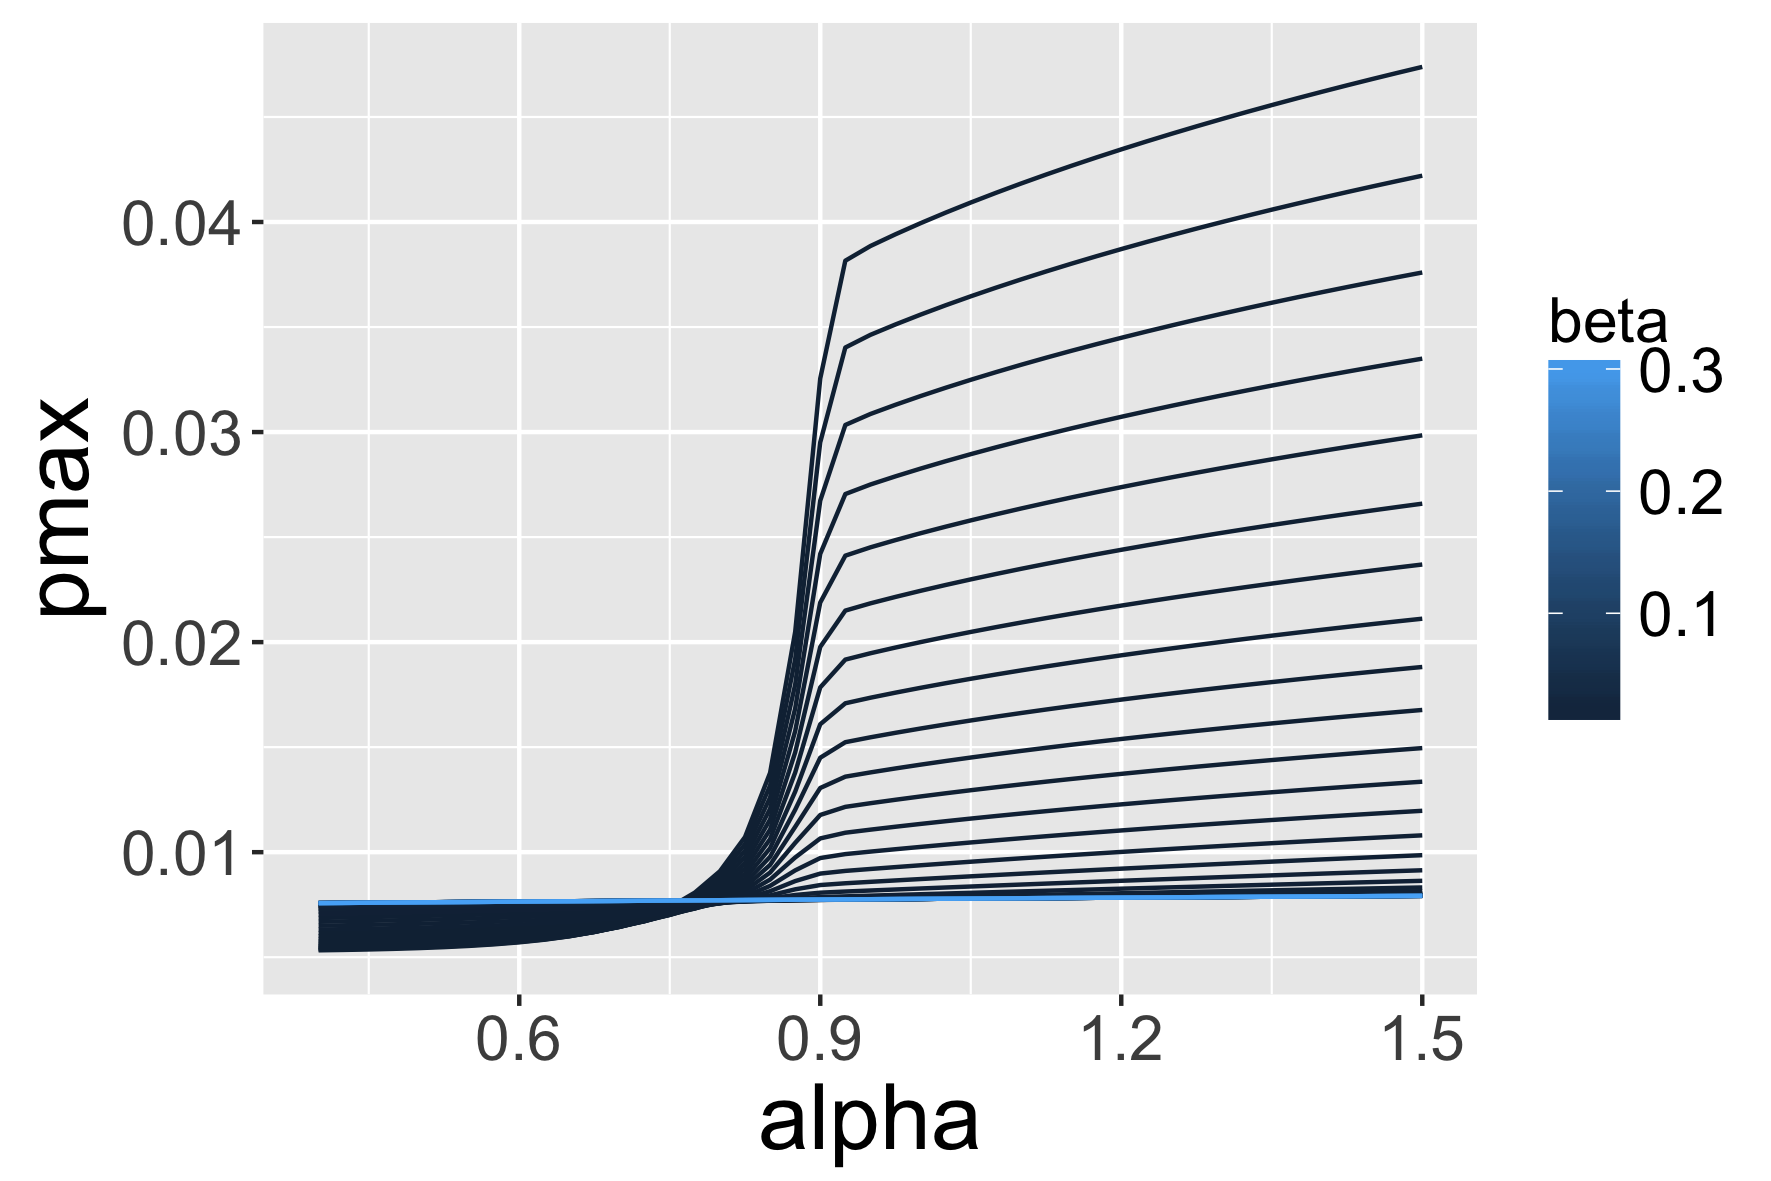
\includegraphics[width=0.49\textwidth]{Figures/Density/pmax_alpha}
%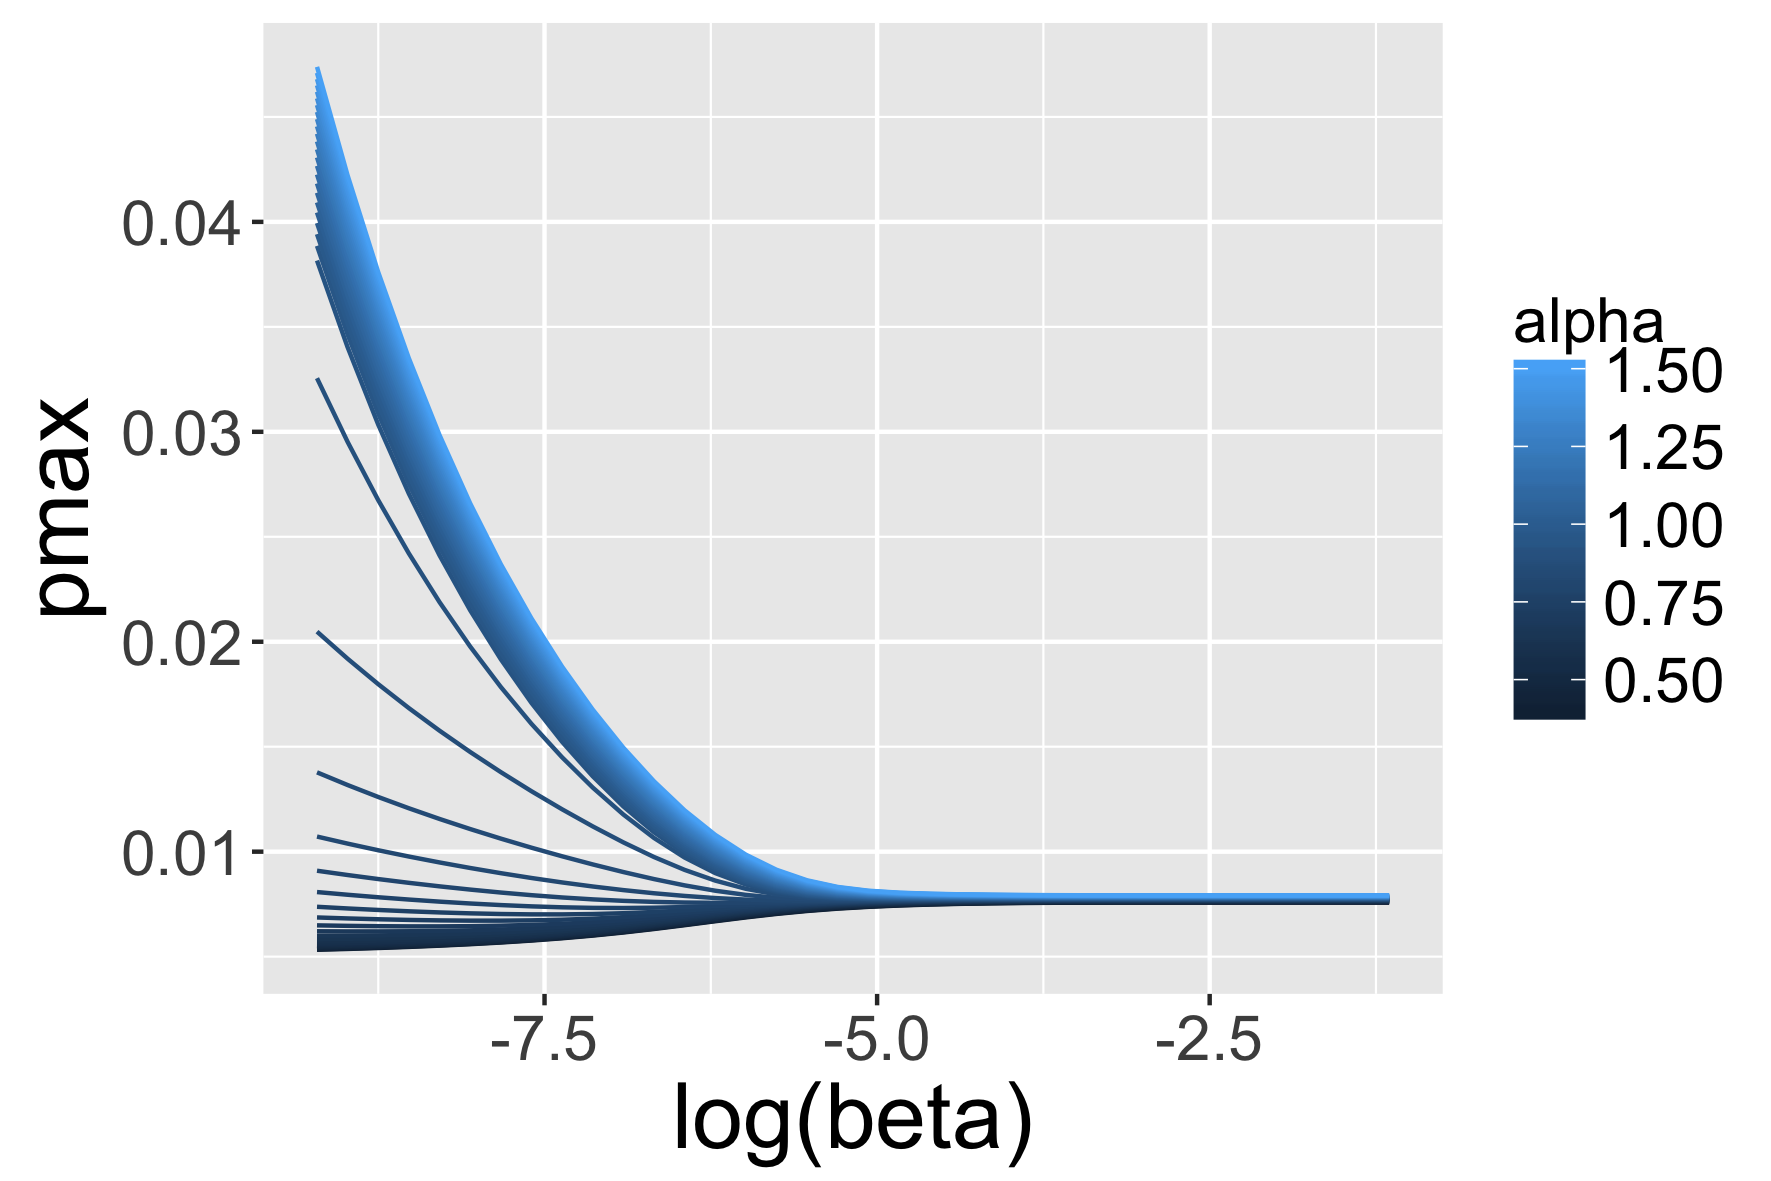
\includegraphics[width=0.49\textwidth]{Figures/Density/pmax_logbeta}
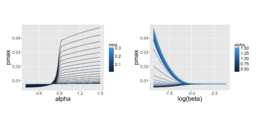
\includegraphics[width=\linewidth]{Figures/Final/A-density-pmax.jpg}
\appcaption{Dependency of $\max d(t\rightarrow \infty )$ to $\alpha$ and $\beta$.\label{fig:app:density:pmax}}{Dépendance de $\max d(t\rightarrow \infty )$ à $\alpha$ et $\beta$.\label{fig:app:density:pmax}}
\end{figure}
%%%%%%%%%%%%%%%%%%%%







%----------------------------------------------------------------------------------------

\newpage

%%%%%%%%%%%%%%%%%%%%%%%
\section{Correlated Synthetic data}{Données Synthétiques Corrélées}

\label{app:sec:correlatedsyntheticdata}


Pour la simulation du couplage faible entre génération d'une configuration de densité et modèle de génération de réseau, la Fig.~\ref{fig:app:correlatedsyntheticdata:correlations} donne les erreurs sur les corrélations faisables montrées en Fig.~\ref{fig:correlatedsyntheticdata:densnwcor}, ainsi que l'amplitude des corrélations pour l'ensemble de la matrice, c'est à dire à la fois la corrélation absolue maximale $c_{ij}=\max_k\left| \rho_{ij}^{k} \right|$ et l'amplitude totale $a_{ij}=\max_k{\rho_{ij}^{(k)}}-\min_k{\rho_{ij}^{(k)}}$.


%%%%%%%%%%%%%%
\begin{figure}
%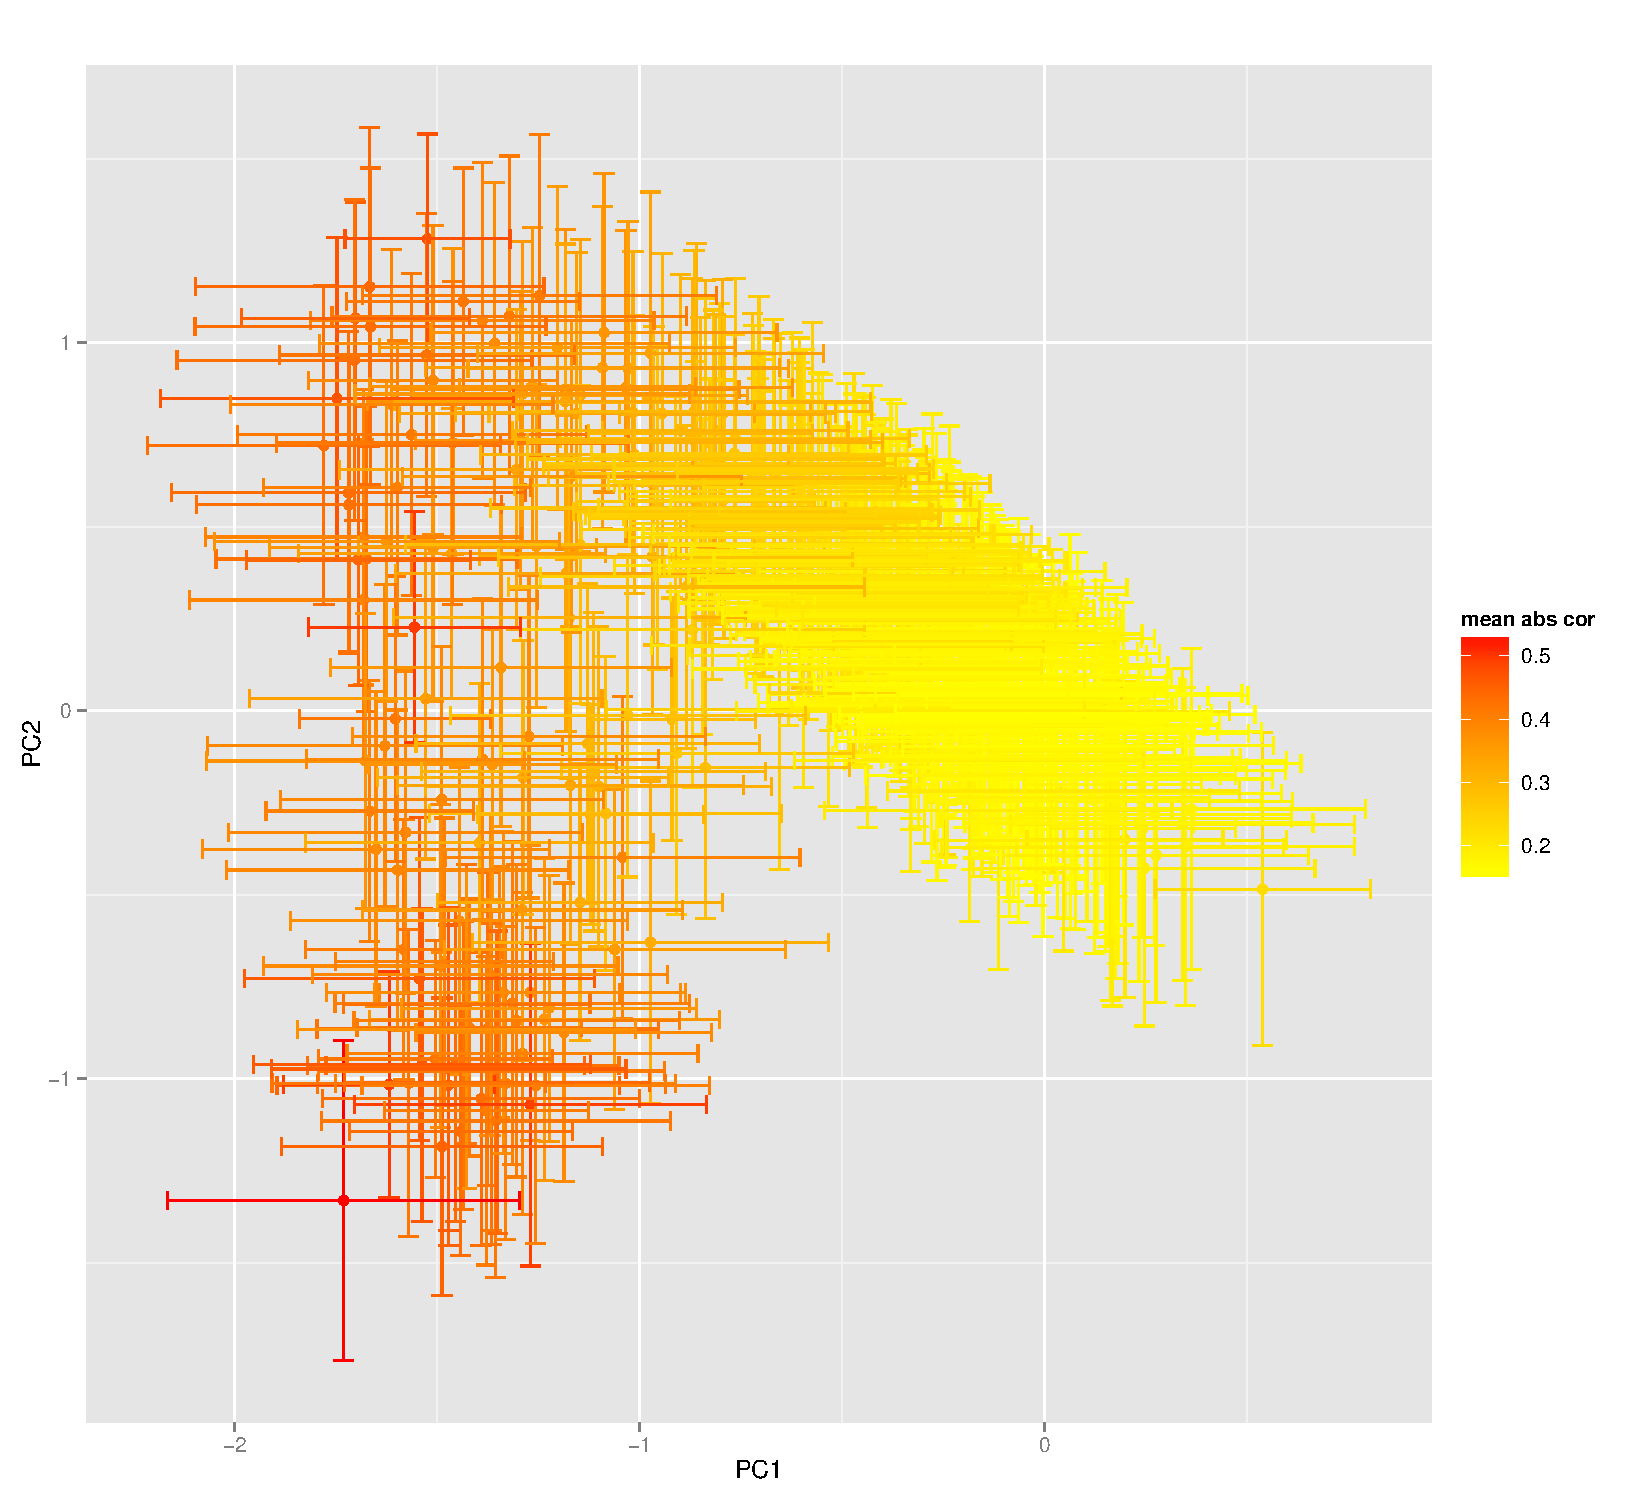
\includegraphics[width=0.48\linewidth]{Figures/CorrelatedSyntheticData/pca_meanAbsCor_errorBars}\\
%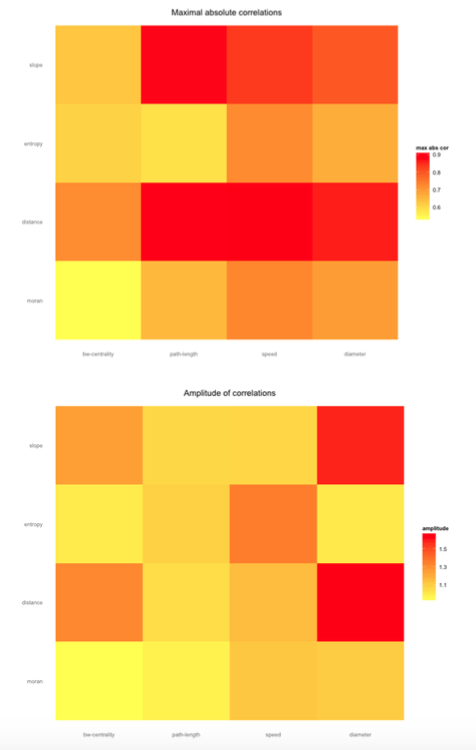
\includegraphics[width=0.31\linewidth]{Figures/CorrelatedSyntheticData/heatmaps}
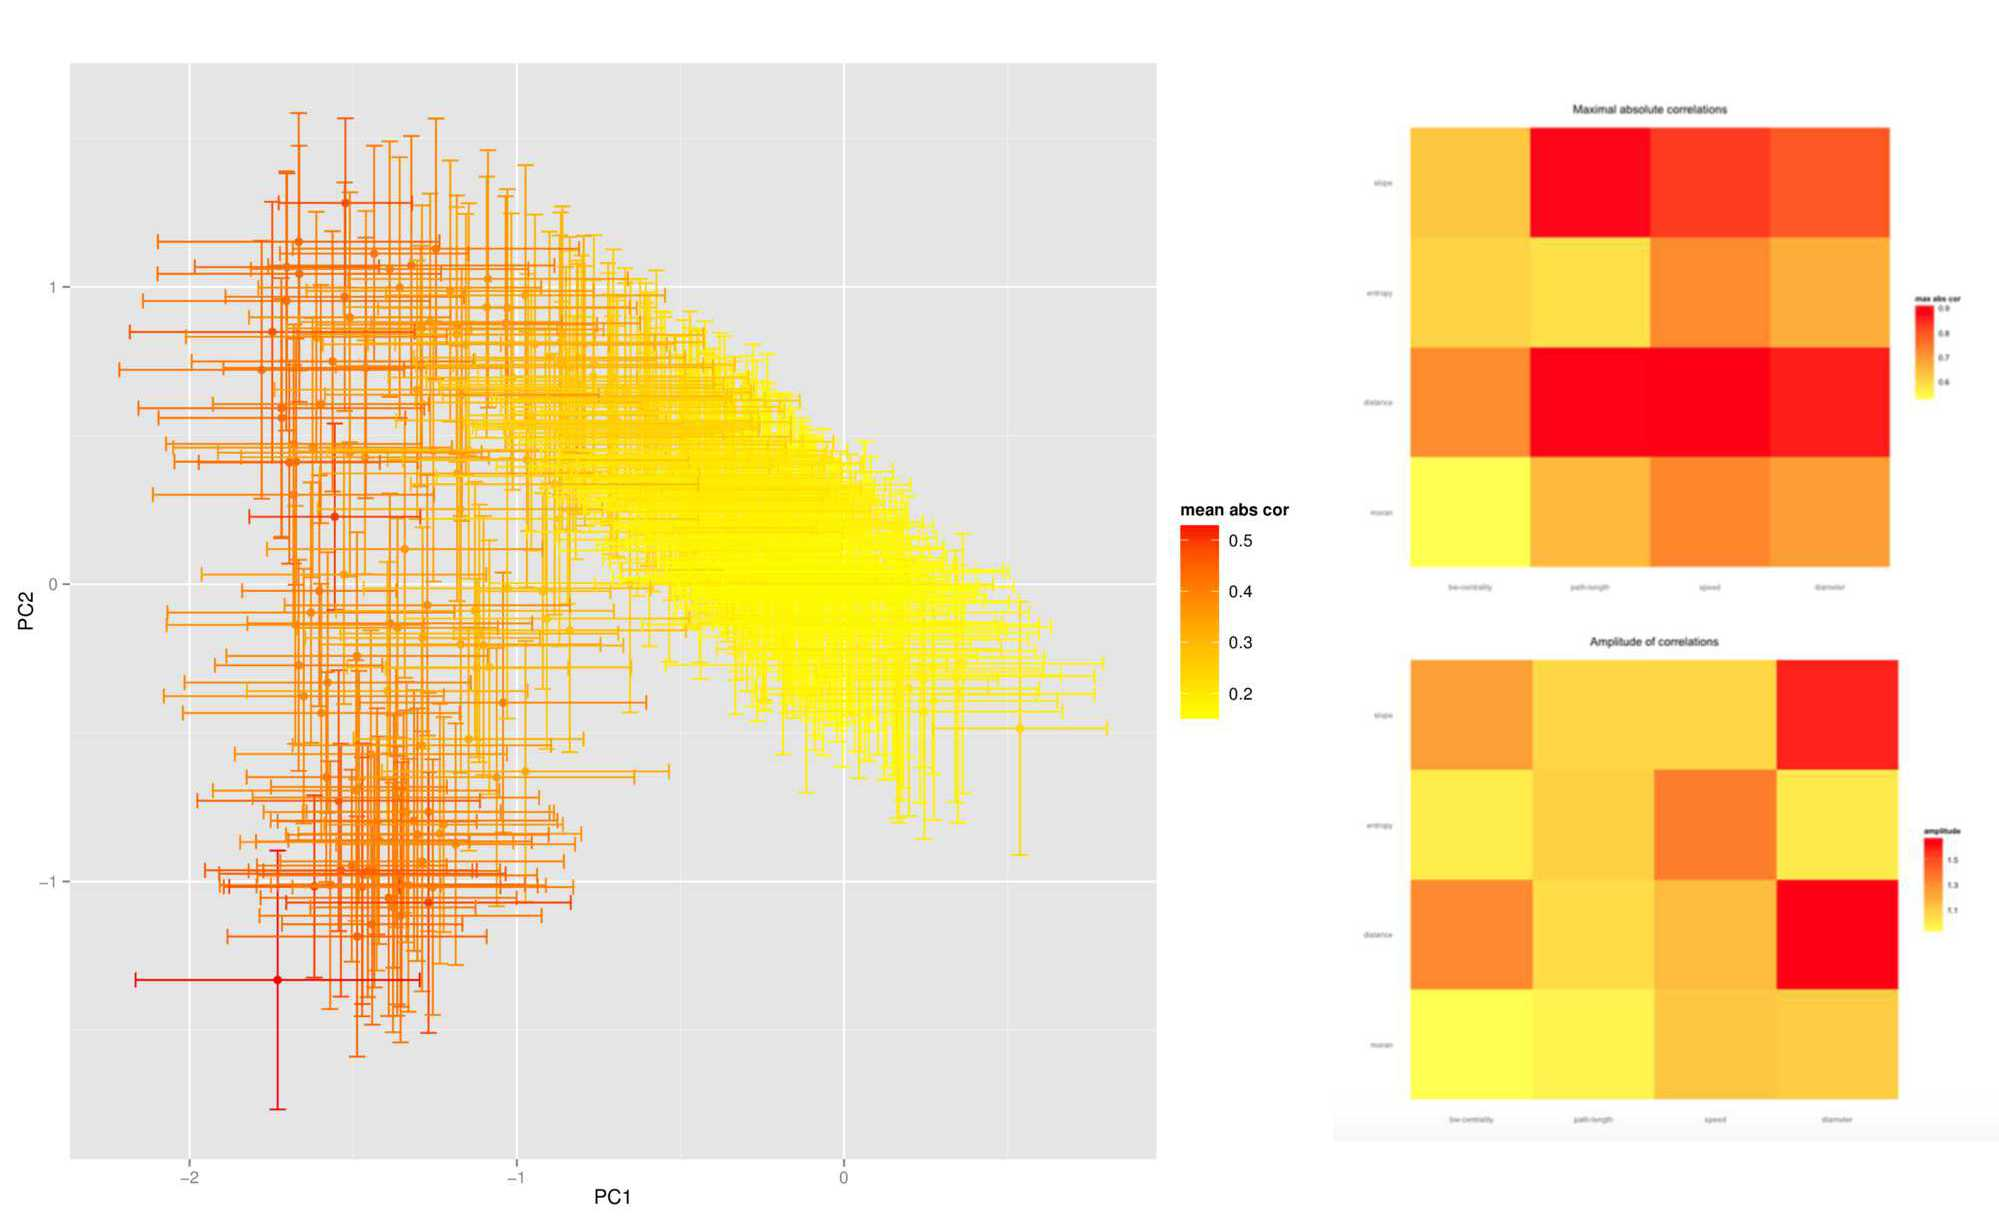
\includegraphics[width=\linewidth]{Figures/Final/A-correlatedsyntheticdata-correlations.jpg}
\appcaption{\textit{(b)} Heatmaps for amplitude of correlations, defined as $a_{ij}=\max_k{\rho_{ij}^{(k)}}-\min_k{\rho_{ij}^{(k)}}$ and maximal absolute correlation, defined as $c_{ij}=\max_k\left| \rho_{ij}^{k} \right|$. \textit{(c)} Projection of correlation matrices in a principal plan obtained by Principal Component Analysis on matrix population (cumulated variances: PC1=38\%, PC2=68\%). Error bars are initially computed as 95\% confidence intervals on each matrix element (by standard Fisher asymptotic method), and upper bounds after transformation are taken in principal plan. Scale color gives mean absolute correlation on full matrices.}{\textbf{Espace des corrélations faisables.}\textit{(Gauche)} Projection des matrices de correlations dans un plan principal obtenu par analyse en composantes principales sur la population des matrices (variances cumulées PC1=38\%, PC2=68\%, s'agissant de corrélations les données sont elles-mêmes corrélées d'où la structure du nuage de points); les barres d'erreur sont calculées initialement comme les intervalles de confiance à 95\% sur chaque matrice (par méthode asymptotique de Fisher standard), et les bornes supérieures après transformation sont prises dans le plan principal; \textit{(Droite)} Amplitude des correlations, définie comme $a_{ij}=\max_k{\rho_{ij}^{(k)}}-\min_k{\rho_{ij}^{(k)}}$ et corrélation maximale absolue, définie comme $c_{ij}=\max_k\left| \rho_{ij}^{k} \right|$ ; l'échelle de couleur donne la corrélation moyenne absolue sur les matrices entières\label{fig:app:correlatedsyntheticdata:correlations}}
\end{figure}
%%%%%%%%%%%%%%









